\documentclass[11pt,a4paper]{memoir}

% set \clubpenalty, etc. to distinctive values for use
% in tracing page breaks. These values are chosen so that
% no single penalty will absolutely prohibit a page break, but
% certain combinations of two or more will.
\clubpenalty=9996
\widowpenalty=9999
\brokenpenalty=4991
% Reiterate the default value of \redisplaypenalty, for
% completeness.
% Set postdisplaypenalty to a fairly high value to discourage a
% page break between a display and a widow line at the end of a
% paragraph.
\predisplaypenalty=10000
\postdisplaypenalty=1549
% And then \displaywidowpenalty should be at least as high as
% \postdisplaypenalty, otherwise in a situation where two displays
% are separated by two lines, TeX will prefer to break between the
% two lines, rather than before the first line.
\displaywidowpenalty=1602

\chapterstyle{hangnum}
\setsecnumdepth{subsubsection}
\setcounter{tocdepth}{3}
\setlength{\footmarkwidth}{0.5em}
\setlength{\footmarksep}{0em}
\setlength{\footparindent}{0em}
\footmarkstyle{\textsuperscript{#1}\hspace{0.5em}}
\newcommand\chap[1]{%
	\chapter*[#1]{#1}%
	\addcontentsline{toc}{chapter}{#1}}

\title{Eslavo Antigo}
\author{Claire Le Feuvre}

\usepackage{pietex}

\usepackage{fontspec}
\usepackage{microtype}
\usepackage[main=brazil]{babel}
\setmainfont{Gentium Plus}
\babelprovide[import, onchar=ids fonts]{ancientgreek}
\babelfont[ancientgreek]{rm}{Brill}
\babeltags{grc = ancientgreek}

\babelprovide[import]{russian}
\babelfont[russian]{rm}{Shafarik}
\babeltags{rus = russian}

\babelprovide{ocs}
\babelfont[ocs]{rm}{Shafarik}
\babeltags{ocs=ocs}

\RequirePackage{graphicx}
% Configurações para o Hyperref
% Paleta de cores
\RequirePackage{xcolor}
\definecolor{green}{RGB}{16, 87, 87} % rgb(16,87,87)

\RequirePackage[pdfusetitle]{hyperref}
\hypersetup{%
	colorlinks=true, % false: boxed links; true: colored links
	linkcolor=green,  % color of internal links
	citecolor=green,  % color of links to bibliography
	filecolor=green,  % color of file links
	urlcolor=green,
}
\renewcommand{\figureautorefname}{Figura}
\renewcommand{\tableautorefname}{Tabela}
\renewcommand{\sectionautorefname}{Seção}
\renewcommand{\chapterautorefname}{Capítulo}
\renewcommand{\subsectionautorefname}{Seção}
\renewcommand{\subsubsectionautorefname}{Pipoca}
\newcommand{\subsubsectionaname}{Seção}
\renewcommand{\appendixpagename}{Apêndices}
\renewcommand{\appendixtocname}{Apêndices}
\renewcommand{\appendixname}{Apêndice}
\renewcommand{\appendixautorefname}{Apêndice}
\newcommand{\aref}[1]{\hyperref[#1]{Apêndice~\ref{#1}}}

\usepackage{paralist}

\let\printindex\undefined
\usepackage{../bibliografia/bibliocaiera}

\usepackage{hyphenat}

\newcommand{\grafema}[1]{$\langle$#1$\rangle$}
\newcommand{\soft}{ь}
\newcommand{\cirilex}[1]{{\rus{}\ciriltrans{#1}}}
\newcommand{\ocsex}[1]{\emph{\ocstrans{#1}}}

\renewcommand{\passagem}[1]{\glslink{idx.#1}{\ifglshasparent{\glsentryparent{idx.#1}}{\glsxtrusefield{\glsentryparent{\glsentryparent{idx.#1}}}{useri}, }{}\glsxtrusefield{\glsentryparent{idx.#1}}{useri}, \gls{idx.#1}}}

\usepackage{lipsum}

\begin{document}

\frontmatter{}
\maketitle

\clearpage
\tableofcontents{}

\mainmatter{}

\pagestyle{companion}
\chapter{Descrição externa}
% TeX root=../main.tex

\section{Apresentação}

O eslavo antigo é uma língua morta, conhecida pelos textos do século X e XI\@.
Os textos eslavos antigos são quase todos textos religiosos traduzidos do grego
e não há literatura original em eslavo antigo.
Os únicos textos originais são inscrições, pouco numerosas, mas nos quais
formulação cristã é de origem grega.

O eslavo antigo foi a língua falada pelos eslavos dos Bálcãs orientais, no
território da atual Bulgária e Macedônia, o que faz com que ele por vezes seja
chamado de búlgaro antigo (\glsxtrshort{alemão}~\emph{Altbulgarisch}).
Uma outra denominação é aquela que não é mais utilizada em francês mas continua
em em uso em alemão em inglês, o eslavão antigo ou o eslavo eclesiástico antigo
(\glsxtrshort{alemão}~\emph{Altkirchenslavisch}, \glsxtrshort{inglês}~\emph{Old Church Slavonic}).
O eslavão (ou no caso os eslavões: eslavão russo, eslavão sérvio etc.), é a
língua litúrgica das igrejas ortodoxas russa, ucraniana, búlgara e sérvia e
representa uma continuação do eslavo antigo, adaptada superficialmente às
particularidades de cada uma das línguas eslávicas.
Neste sentido, as variantes modernizadas do eslavo antigo persistiram até que a
língua se tornasse morta, mas em um contexto extremamente restrito de uso
litúrgico.

Apontamos tradicionalmente o fim do eslavo antigo e a passagem ao búlgaro
moderno no fim do século XI\@.

\section{Notas históricas}

Os falantes dessa língua são divididos essencialmente em três grupos étnicos.
As tribos eslávicas chegam ao leste dos Balcãs ao fim do século V, sendo a
principal a dos severianos, que significa ``os do norte'' (outros severianos se
encontram no território), cf.~\autoref{fig:eslavos_sec8_9}.
Esses eslavos se instalam em um território ocupado por trácios que são
rapidamente assimilados.
Eles engajam em saques pelos Balcãs, quase chegando ao Peloponeso.
Por volta do meio do século VII, uma população asiática de origem
turco-mongólica, os búlgaros, chega e impõe sua dominação sobre os eslavos (isto
é, aos eslavos propriamente ditos e aos trácios eslavizados).

\begin{figure}[!htb]
  \begin{center}
    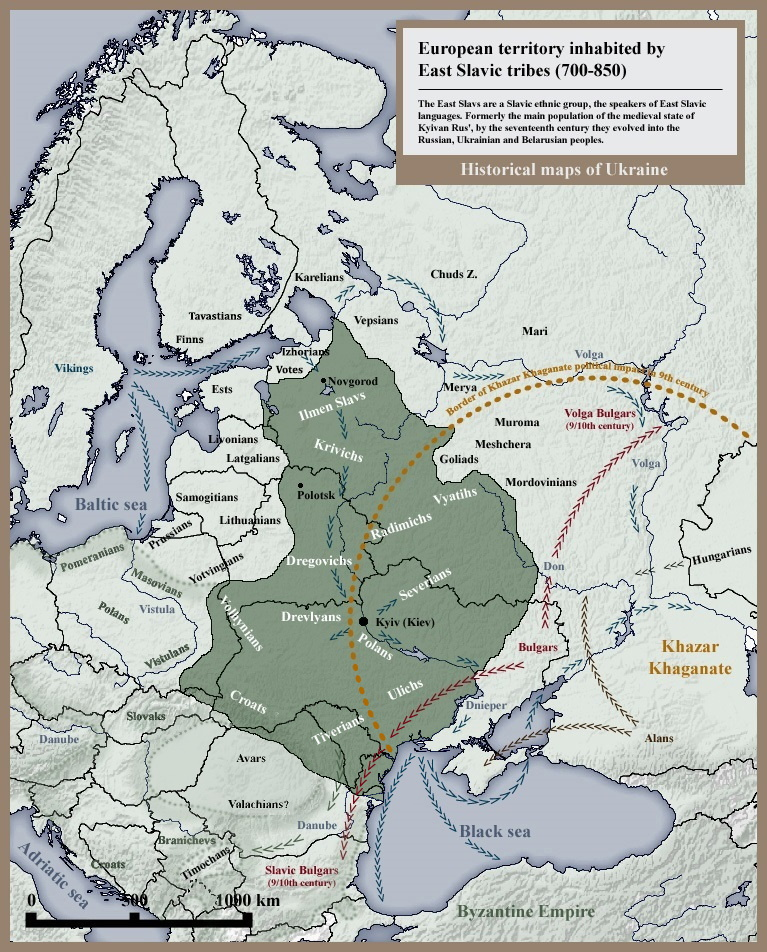
\includegraphics[width=0.75\textwidth]{assets/East_Slavic_tribes_peoples_8th_9th_century.jpg}
  \end{center}
  \caption{Eslavos durante os séculos VIII-IX\@. Fonte: \url{https://pt.wikipedia.org/wiki/Ficheiro:East_Slavic_tribes_peoples_8th_9th_century.jpg}}\label{fig:eslavos_sec8_9}
\end{figure}


A fundação do reino da Bulgária se segue à vitória do khan Asparuch sobre o
imperador bizantino Constantino IV em 680.
Esses búlgaros, que deram seu nome ao país, são rapidamente eslavizados por sua
vez.
Para evitar a confusão, chamamos a língua desse povo de ``proto-búlgaro'',
aparentada ao turco e separamos o termo ``búlgaro antigo'' à língua eslava, seja
como um equivalente ao ``eslavo antigo'' em sua totalidade, seja para designar o
dialeto búlgaro do eslavo antigo em oposição ao dialeto macedônio, o que será
útil aqui.

Em 862, o príncipe da Morávia (Chéquia atual), buscando aliança com Bizâncio para
se opor à crescente influência dos francos e da Igreja de Roma, pede ao
imperador bizantino Miguel III que envie missionários à Morávia.
Miguel incumbe dois monges de origem eslava da Tessalônica, Constantino (Cirilo
é seu nome de monge) e seu irmão Metódio de criar um alfabeto para o eslavo e
traduzir os evangelhos a essa língua. 
A missão na Morávia começa em 863.
Cirilo morre em 869, Metódio permanece na Morávia mas após sua morte em 885 seus
discípulos são perseguidos e se refugiam na Bulgária, que se torna o centro das
letras eslavas.

Um pouco antes deste momento, o reino da Bulgária, cuja capital é Pliska,
torna-se oficialmente cristão, em 864, com o batismo do rei Boris I (852--889).
O filho mais velho de Boris, Vladmir, o sucede brevemente, mas é deposto quatro
anos mais tarde.
Seu irmão Simeão (893--927) o sucede: inicialmente destinado a uma vida
monástica, Simeão é um letrado perfeitamente helenizado que havia estuado dez
anos em Constantinopla.
Ele move a capital para Preslav (Preslav Veliki ou Grande Preslav) desde o
início de seu reinado.
Aproveitando a presença dos discípulos de Cirilo e Metódio expulsos da Morávia
(885), Simeão torna Preslav em um centro cultural importante, onde a atividade
de cópia e tradução de textos gregos estava em pleno vapor.
Simeão se encarrega de favorecer o desenvolvimento das letras eslavas, afirmando
o prestígio de seu reino e firmando sua independência política frente a
Bizâncio: a Igreja búlgara se torna autônoma com relação à hierarquia grega,
depois autocéfala a partir de 915, e Simeão toma o título de imperador
(\ocsex{cEsar'I}) em 913.
Sob seu regime, o reino da Bulgária alcança seu apogeu e se estende desde o Mar
Negro ao Adriático (\emph{cf.}~\autoref{fig:reino_bulgaria})
Sob o sucessor de Simeão, seu filho Pedro I (927--969), a agitação social toma o
reino.
Após uma revolta na Macedônia ao final do século X, uma nova dinastia se instala
com o rei Samuel (976--1014), que move o centro de poder à Macedônia, na direção
do sudeste, e faz de Ohrid sua capital.
Mas o reino é subjugado por Bizâncio em 1014 e o imperador Basílio II ganha o
sobrenome de Bulgarotóctone.
Samuel morre um pouco depois da derrota.
Um  segundo reino da Bulgária se reconstitui no final do século XII (1186) e
tem por capital Tărnovo, que durará até a conquista turca em 1393.
Esse segundo reino da Bulgária corresponde ao período búlgaro moderno e a língua
desta época ja não é mais o eslavo antigo.

\begin{figure}[!htb]
  \begin{center}
    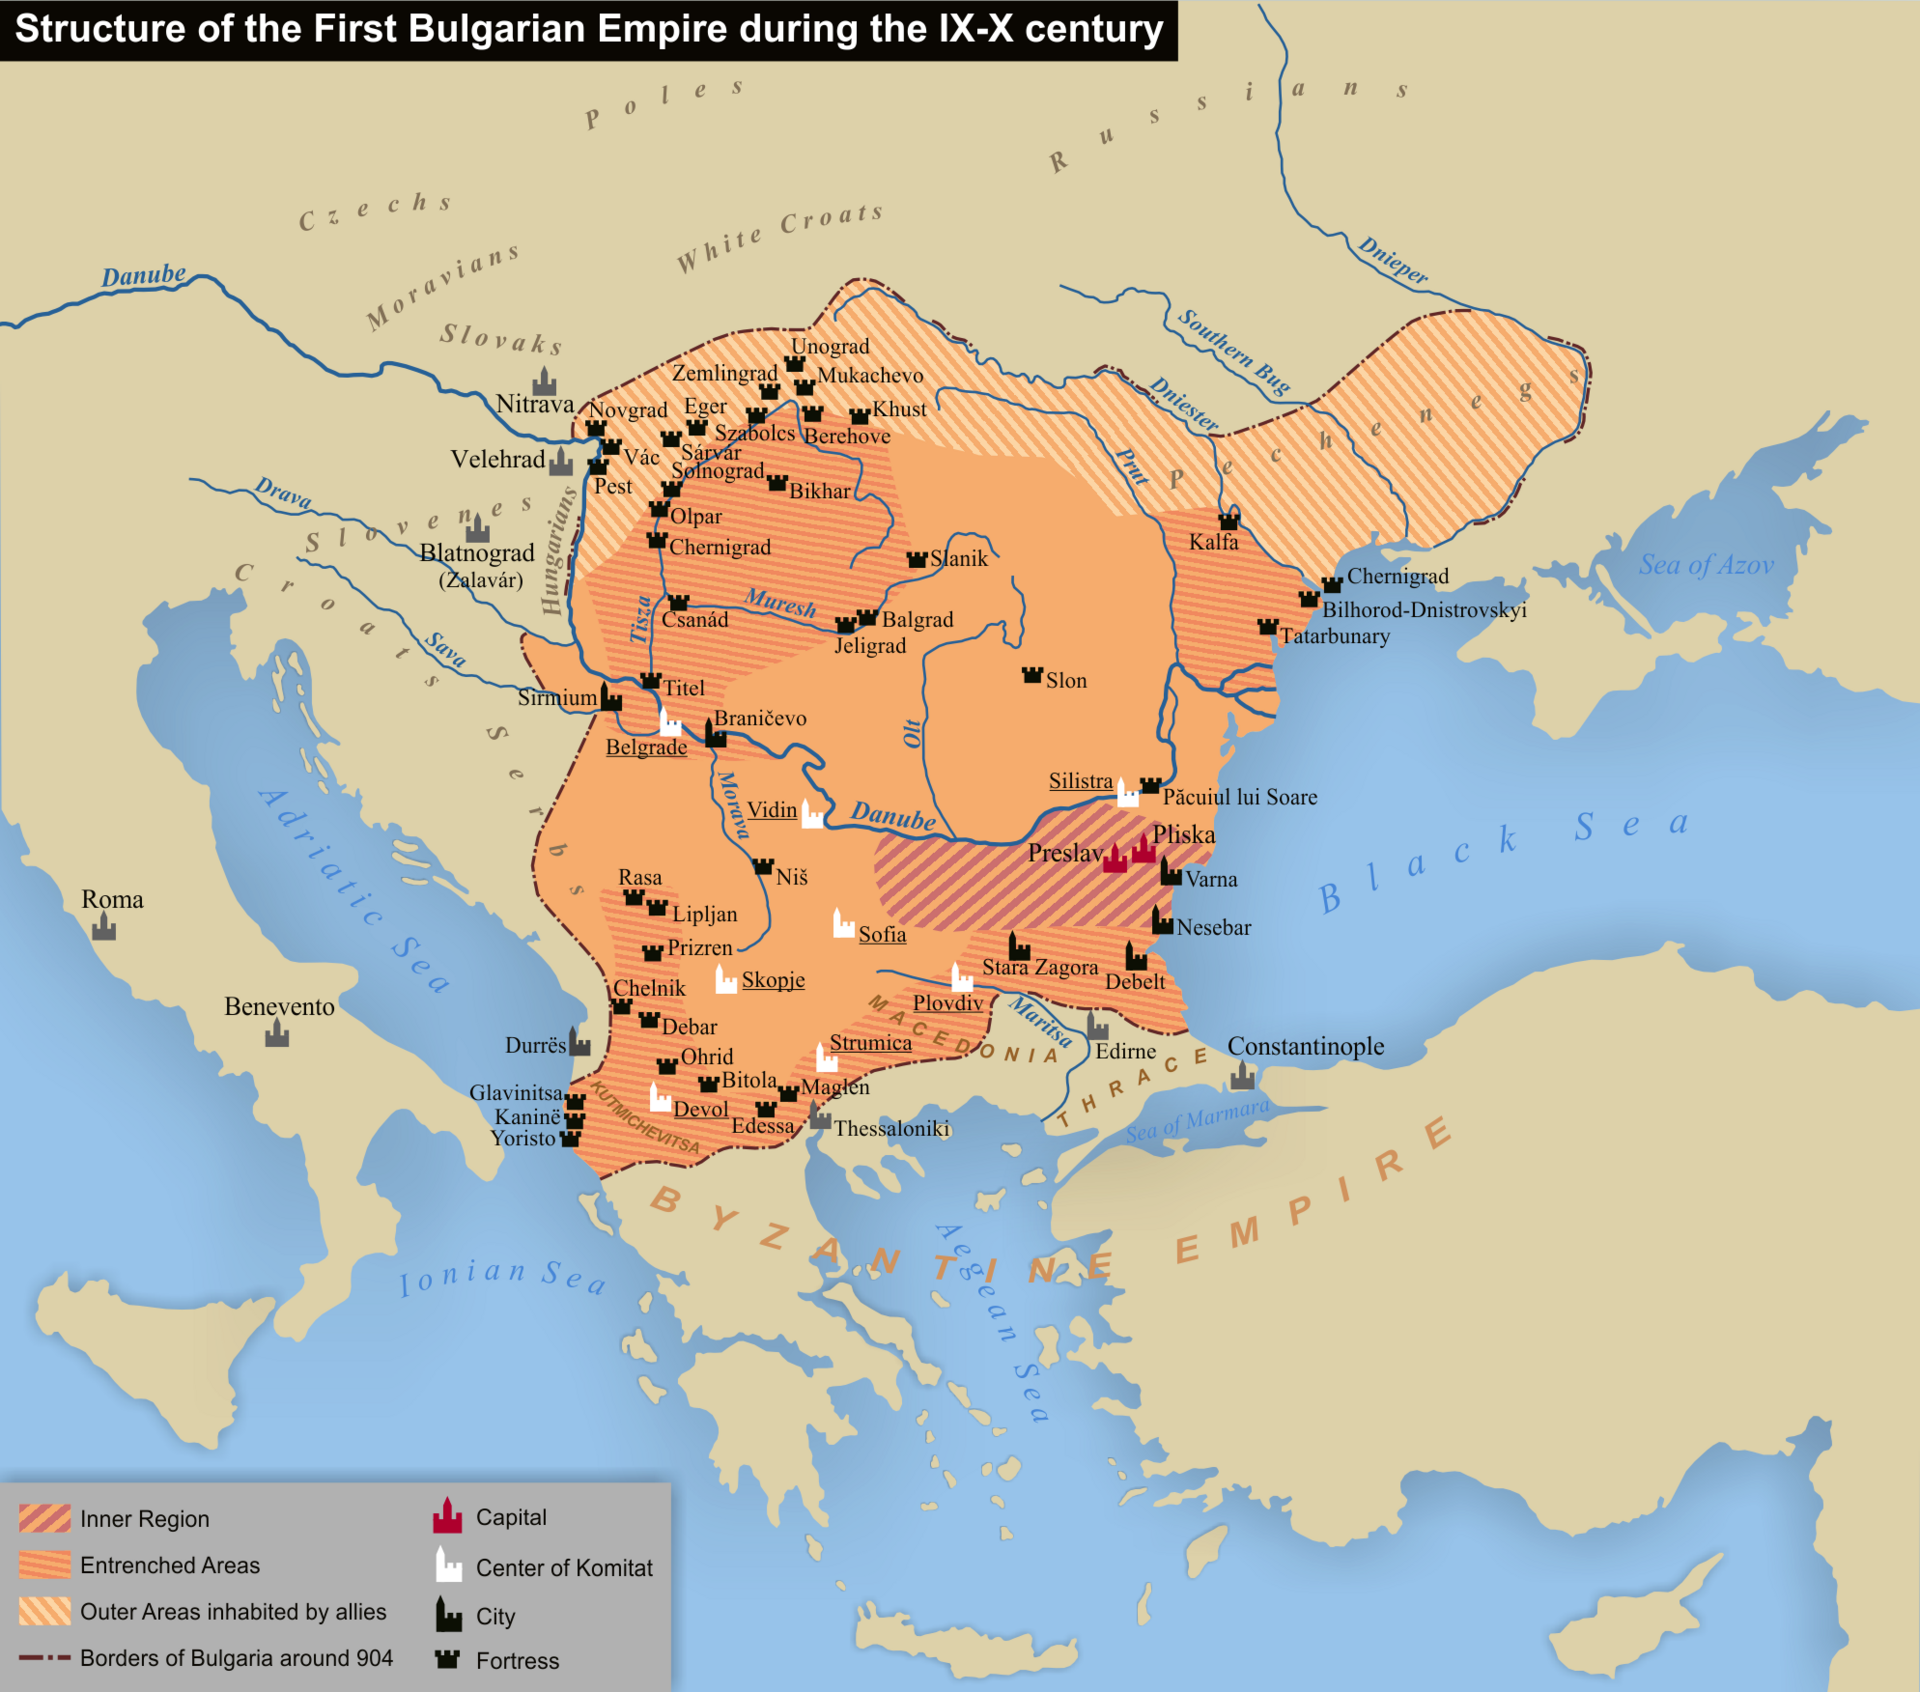
\includegraphics[width=0.75\textwidth]{assets/Structure_of_the_First_Bulgarian_Empire_during_the_IX-X_century.png}
  \end{center}
  \caption{Primeiro reino búlgaro. Fonte: \url{https://commons.wikimedia.org/wiki/File:Structure_of_the_First_Bulgarian_Empire_during_the_IX-X_century.png}}\label{fig:reino_bulgaria}
\end{figure}

\section{Grafia}

O eslavo antigo é grafado com dois alfabetos diferentes, que se sucedem e que
coexistiram durante um certo tempo (ver~\autoref{tab:alfabetos}).
O primeiro, inventado por Constantino-Cirilo segundo a tradição, é o alfabeto
glagolítico (também chamado glagolito), nome que, tal como cirílico para o outro
sistema, é tardio.
É um sistema único que não corresponde a qualquer outro sistema alfabético
contemporâneo conhecido.
As fontes do alfabeto glagolítico são disputadas.
Para alguns, trata-se de uma criação \emph{ex nihilo} de Cirilo, enquanto para
outros ele seria inspirado na escrita siríaca e para outros ainda essa escrita
seria derivada da cursiva grega.
Essa última tese, a mais difundida, tem voltado a ser favorecida~\cite[para o estado
da questão, ver][]{Marti2004}.
Não temos nenhum traço de escrita eslava antes de Cirilo, mas o alfabeto grego
era utilizado para representar o eslavo, de modo que a vemos em algumas
inscrições, e é possível que Cirilo não tenha feito nada se não dar a forma
definitiva a um sistema esboçado por outros.
A escrita glagolítica continua sendo usada na Croácia até o começo do século XX
em uma variante conhecida por ``glagolito quadrado'', por conta do formato de
suas letras.

Noutras regiões, ela é no entanto rapidamente abandonada e substituída por um
outro sistema, o alfabeto chamado cirílico (mesmo ele não sendo invenção de
Cirilo mas de seus sucessores), derivado da uncial grega.
Os fonemas que fossem idênticos em eslavo e em grego são notados pela letra
grega correspondente: por isso das vogais \emph{a}, \emph{e}, \emph{i},
\emph{o}, os dois últimos fonemas são notados por dois grafemas diferentes,
transpondo a situação do grego: 
\grafema{{\rus{}Ꙇ}} e \grafema{{\rus{}И}} para /i/ (grego \grafema{Ι} e
\grafema{Η}, pronunciado [i] por causa do iotacismo), \grafema{{\rus{}О}} e
\grafema{{\rus{}Ѡ}} para /o/, enquanto para \emph{u} há a notação
\grafema{{\rus{}ОУ}}, calque do dígrafo grego \grafema{ΟΥ};
os dois grafemas para /i/ e /o/ existem igualmente em glagolítico e o grafema
para /u/ em glagolítico é claramente uma ligatura em que o primeiro elemento é o
grafema para /o/, o que advoga em favor da tese de que o alfabeto glagolítico
seja derivado do grego.
De mesma maneira, a maior pare das consoantes do cirílico conservam a forma de
seu modelo grego.
A notação de fonemas que não teriam correspondente em grego (por exemplo as
fricativas \emph{š}, \emph{ž}, \emph{č}, a africada \emph{c} e as vogais nasais
\emph{ę} e \emph{ǫ}) se faz por meio de grafemas do alfabeto glagolítico.


\begin{table}[!htb]
  \caption{Alfabetos cirílico e glagolítico}\label{tab:alfabetos}
  \begin{center}
    \begin{tabular}[c]{llll||llll}
      \toprule
      glagolítico & cirílico & translit. & IPA & glagolítico & cirílico &
      translit. & IPA\\
      \midrule
      {\ocs{}Ⰰ}   & {\rus{}А} & a  & [a]   & {\ocs{}Ⱆ} & {\rus{}ОУ Ꙋ}  & u    & [u]\\
      {\ocs{}Ⰱ}   & {\rus{}Б} & b  & [b]   & {\ocs{}Ⱇ} & {\rus{}Ф}     & f    & [f]\\
      {\ocs{}Ⰲ}   & {\rus{}В} & v  & [v]   & {\ocs{}Ⱈ} & {\rus{}Х}     & x    & [x]\\
      {\ocs{}Ⰳ}   & {\rus{}Г} & g  & [g]   & {\ocs{}Ⱌ} & {\rus{}Ц}     & c    & [ts]\\
      {\ocs{}Ⰴ}   & {\rus{}Д} & d  & [d]   & {\ocs{}Ⱍ} & {\rus{}Ч}     & č    & [tʃ,]\\
      {\ocs{}Ⰵ}   & {\rus{}Є} & e  & [ʲe]  & {\ocs{}Ⱎ} & {\rus{}Ш}     & š    & [ʃ,]\\
      {\ocs{}Ⰶ}   & {\rus{}Ж} & ž  & [ʒ]   & {\ocs{}Ⱋ} & {\rus{}щ}     & št   & [ʃt,]\\
      {\ocs{}Ⰷ}   & {\rus{}Ѕ} & dz & [dz,] & {\ocs{}Ⱏ} & {\rus{}Ъ}     & ŭ, ъ & [ə]\\
      {\ocs{}Ⰸ}   & {\rus{}З} & z  & [z]   & {\ocs{}ⰟⰊ } & {\rus{}Ꙑ ЪИ}     & y    &\\
      {\ocs{}Ⰹ Ⰺ} & {\rus{}И} & i  & [i]   & {\ocs{}Ⱐ} & {\rus{}Ь}     & ĭ    & [ʲe]\\
      {\ocs{}Ⰻ}   & {\rus{}Ꙇ} & i  & [i]   & {\ocs{}Ⱑ} & {\rus{}Ѣ}     & ě    & [ʲa]\\
      {\ocs{}Ⰼ}   & {\rus{}Ћ} & g' & [g,]  & {\ocs{}Ⱓ} & {\rus{}Ю}     & ju   & [ju]\\
      {\ocs{}Ⰽ}   & {\rus{}К} & k  & [k]   & {\ocs{}}  & {\rus{}Ꙗ}     & ja   & [ja]\\
      {\ocs{}Ⰾ}   & {\rus{}Л} & l  & [l]   & {\ocs{}}  & {\rus{}Ѥ}     & je   & [je]\\
                  & {\rus{}Л҄} & l' & [l']  & {\ocs{}Ⱔ} & {\rus{}Ѧ}     & ę    & [ɛ̃]\\
      {\ocs{}Ⰿ}   & {\rus{}М} & m  & [m]   & {\ocs{}Ⱗ} & {\rus{}Ѩ}     & ję   & [jɛ̃]\\
      {\ocs{}Ⱀ}   & {\rus{}Н} & n  & [n]   & {\ocs{}Ⱘ} & {\rus{}Ѫ}     & ǫ    & [ɔ̃]\\
                  & {\rus{}Н҄} & n' & [n,]  & {\ocs{}Ⱙ} & {\rus{}Ѭ}     & jǫ   & [jɔ̃]\\
      {\ocs{}Ⱁ}   & {\rus{}О} & o  & [ɔ]   & {\ocs{}Ⰰ} & {\rus{}Ѯ}     & ks   & [ks]\\
      {\ocs{}Ⱂ}   & {\rus{}П} & p  & [p]   & {\ocs{}Ⰰ} & {\rus{}Ѱ}     & ps   & [ps]\\
      {\ocs{}Ⱃ}   & {\rus{}Р} & r  & [r]   & {\ocs{}Ⱚ} & {\rus{}Ѳ}     & t    & [t]\\
                  & {\rus{}Р҄} & r' & [r,]  & {\ocs{}Ⱛ} & {\rus{}Ѵ}     & u    & [u]\\
      {\ocs{}Ⱄ}   & {\rus{}С} & s  & [s]   & {\ocs{}Ⱉ} & {\rus{}Ѡ}     & o    & [o]\\
      {\ocs{}Ⱅ}   & {\rus{}Т} & t  & [t]   &  &  &   &    \\
      \bottomrule
    \end{tabular}
  \end{center}
\end{table}

Como em grego, as letras possuem também um valor numérico.
No alfabeto glagolítico, o valor segue a ordem das letras (\grafema{a} = 1,
\grafema{b} = 2, \grafema{v} = 3, \grafema{g} = 4, etc), mas no alfabeto
cirílico o valor é calcado naquele da letra grega, de modo que há um salto de
uma unidade com relação ao valor numérico do glagolítico (assim, é
{\rus{}В}\slash{}\emph{v} que vale 2, e não {\rus{}Б}\slash{}\emph{b}, que não possui valor
numérico, {\rus{}Г}\slash{}\emph{g} = 3, etc.).

Nos manuscritos tanto em glagolítico como em cirílico, o uso de abreviações para
palavras comuns, à imitação do grego, é constante: a abreviação é sinalizada
pelo \emph{titulus}, um sinal \grafema{{\rus{} ҃  }}, colocado acima da palavra abreviada.

O alfabeto cirílico, que é assim um alfabeto misto, deve ter se formado no
contexto bilíngue dos eslavos helenizados.
Seus primeiro traços epigráficos datam do século X\@: a mais antiga inscrição em
cirílico é datada de 921.
A sua simplicidade e o prestígio que lhe conferia seu modelo grego garantiram
seu sucesso e logo foram refeitas cópias em que se transcrevia em cirílico os
antigos manuscritos em glagolítico.
É difícil dizer se ocorreu uma política deliberada para impor o alfabeto
cirílico: no máximo pode-se concluir a partir do celo do rei Pedro (morto em
969) e da inscrição de Samuel de 993, ambos em cirílico, que os soberanos eles
mesmos, ao utilizarem o alfabeto cirílico como alfabeto oficial em alguma
medida, contribuíram para sua propagação.
No entanto, os tradutores e copistas da escola de Ohrid mantiveram o uso do
glagolítico.
A maior parte dos textos eslavos antigos conservados estão em glagolítico (ver
abaixo), o que se explica pelo fato de que nos foram conservados sobretudo os
texto do período macedônio, da escola de Ohrid.
Nas inscrições de Preslav dos séculos IX e X, os dois sistemas coexistem.

Fora dos Balcãs, encontram-se algumas inscrições glagolíticas na Rússia, em Santa
Sofia de Kiev e em Novgorod, mas elas são muito pouco numerosas e o cirílico que
se impõe desde os primeiros textos.
Por outro lado, o \emph{Codex de Novgorod} ou \emph{Saltério de Novgorod} (três
tabuletas de madeira cobertas por cera com quatro faces inscritas), descoberto
em 2000 (e que por isso não são listados em \textcite{Schenker1995} nem em
\textcite{BirnbaumSchaeken1999}), fragmento de um saltério em eslavo antigo,
está em cirílico: data-se eles do primeiro quarto do século XI e eles assim se
juntam aos documentos mais antigos em eslavo antigo conservados (edição
provisória de A.~A.\ Zalizniak e V.~L.\ Janin em \emph{Voprosy Jazykoznanija}
(2001/5: 3--25)).
O texto difere ligeiramente daquele do \emph{Saltério do Sinai}, o que atesta
duas tradições eslavas distintas.
Na medida em que o texto não provém da região da Bulgária\hyp{}Macedônia, mas
foi escrito por um russo e apresenta assim alguns traços do eslavo oriental, não
o incluiremos à lista de textos em eslavo antigo canônicos.

\section{Documentos}

O corpus eslavo antigo \emph{stricto sensu} é constituído por um número limitado
de textos de extensão desigual, que constituem o ``cânone'' ao qual se somam
algumas inscrições conservadas.
Encontrar-se-á uma descrição dos textos e das edições modernas
em~\textcite[87--130]{BirnbaumSchaeken1999}, que integra os documentos
descobertos depois da publicação do \emph{Manuel du vieux slave} de Vaillant.

\subsection{O cânone clássico}

\begin{compactitem}[--]
    \item \emph{Folhas de Kiev} (ou \glsxtrlong{Kiev}) [\glsxtrshort{Kiev}],
      fragmento de missal seguindo o rito romano, traduzido do latim, em eslavão
      morávio (7 fol., glagol., séc.\ X),
      é o texto mais antigo e conservado e o único que atesta diretamente a
      tradição morávia. Ed. J. Schaeken, \emph{Die Kiever Blätter}, Amsterdam, 1987.
    \item \glsxtrlong{Zogr} [\glsxtrshort{Zogr}], quatro evangelhos (270 fol.,
      glagol., final do séc.\ X--começo do XI, Macedônia, provavelmente o manuscrito
      mais antigo conservado depois do 
      \glsxtrlong{Kiev}). Ed. V. Jagic, \emph{Quattuor evangeliorum codex
      glagoliticus olim Zographensis nunc Petropolitanus}, Berlim, 1879
      (transcrição cirílica).
    \item \glsxtrlong{Marianus} [\glsxtrshort{Marianus}], quatro evangelhos (171 + 2 fol., faltam os
      capítulos de 1 a 5 e 24 de Mateus, glagol., final do séc.\ X--começo do
      XI, Macedônia, provavelmente posterior ao \glsxtrshort{Zogr}). Ed. V. Jagic,
      \emph{Mariinskoe četveroevangelie, s primečanijami i s priloženijami}, S.
      Petersburgo 1883 (transcrição cirílica, glossário, aparato crítico com
      leituras divergentes de \glsxtrshort{Zogr}, \glsxtrshort{Assemanius}, \glsxtrshort{Sav} e do
      \emph{Evangelho de Ostromir}).
    \item \glsxtrlong{Assemanius} [\glsxtrshort{Assemanius}], evangeliários (158 fol., glagol.,
      XI, Macedônia). Ed. J. Vajs, J. Kurz, \emph{Evangeliář Assemanuv, Kodex
      Vatikánský 3.\ slovanský}, Praga, 1929-1955 (fac-símile, transcrição cirílica).
    \item \glsxtrlong{Sav} [\glsxtrshort{Sav}], evangeliário (130 fol., ciríl., XI°,
      Bulgária). Ed. O.~A.\ Knjazevskaja \emph{et al.}, \emph{Savvina kniga,
      drevneslavjanskaja rukopis’ XI, XI- XII i konca XIII veka}, Moscou, 1999 —
      (vol.\ 1: fac-símile, texto, comentários).
    \item Palimpsesto do Vaticano, fragmento de evangeliário (93 fol., ciríl.,
      final do séc.\ X--começo do XI, Bulgária). Ed. T. Kraštanov \emph{et al.},
      \emph{Vatikansko evangelie. Starobălgarski kirilski aprakos ot X.\ v.\ v
      palimpsesten Kodeks Vat.\ Gr.\ 2502}, Sofia, 1996 (apenas texto).
    \item \emph{Folhas de Ohrid}, fragmento de evangeliário e de lecionário (2
      fol., glagol., XI, Macedônia). Ed. T.~A.\ Lysaght, \emph{A selection of
      ancient Slav literary monuments incorporating Monumenta minora palaeobulgaricae}, Vienne 1982 (transcrição cirílica, fac-símile).
    \item \emph{Fragmento do Sinai}, fragmento de evangeliário (1 fol., glagol.,
      segunda metade do século XI). Ed.\ M. Altbauer, V. Mareš, ``Fragmentum
      glagoliticum evangeliarii palæoslovenici in codice Sinaitico 39
      (palimpsestum)'', Viena, 1980 (transcrição cirílica, fac-símile); com
      complementos dos mesmos em \emph{Wiener Slawistischer Almanach} 7, 1981.
    \item \emph{Saltério do Sinai} [\emph{Ps.}] (209 fol., glagol., XI,
      Macedônia). Ed.\  I.~C.\ Tarnanidis, \emph{The Slavonic manuscripts
      discovered in 1975 at St Catherine's Monastery on Mount Sinai},
      Tessalônica 1988 (para a primeira parte do manuscrito), F. Mareš,
      \emph{Psalterii Sinaitici pars nova}, Viena, 1997 (para a segunda parte)
      (introdução, transcrição cirílica, aparato crítico, concordância).
    \item \emph{Euchologe do Sinai} [\emph{Euch.}] (133 + 1 fol., glagol., XI,
      Macedônia). Ed.\ J. Frèek, \emph{Euchologium Sinaiticum. Texte slave avec
      sources grecques et traduction française}, Paris 1933-1939 (transcrição
      cirĺica, texto grego, tradução francesa); R. Nahtigal, \emph{Euchologium
      Sinaiticum. Starocerkvenoslovanski rlagoiski spomenik}, Ljubljana,
      1941-1942 (transcrição cirílica, fac-símile, glossário).
    \item \emph{Missal do Sinai} (80 fol., glagol, XI, Macedônia?). Ed.\ edição
      parcial, Tarnanidis 1988 (\emph{cf}.\ \emph{Saltério}).
    \item \glsxtrlong{Supr} [\glsxtrshort{Supr}], menólogo de \emph{mars} e
      homilías (118 + 16 + 151 fol., ciríl., XI, Bulgária), um dos manuscritos
      mais recentes, posterior a \glsxtrshort{Sav} Ed.\ J. Zaimov, M. Capaldo,
      \emph{Suprasǎlski ili Retkov sbornik}, Sofia, 1982--1983 (fac-símile,
      comentário, texto grego).
    \item \glsxtrlong{Clozianus} [\glsxtrshort{Clozianus}], fragmento de homiliário (12 + 2 fol.,
      glagol., XI, Macedônia). Ed.\ Dostál 1959 (transcrição cirílica e latina,
      texto grego e latino, tradução checa, fac-símile, glossário).
    \item \emph{Folhas de Rila} (1 + 6 fol., glagol., XI, Macedônia). Ed.\ I.\
      Gotev, \emph{Rilski glagoliceski listove}, Sofia, 1956 (transcrição
      cirílica, fac-símile, glossário).
    \item \emph{Folhas de Hilandar}, fragmento de Cirilo de Jerusalém (2 fol.,
      ciríl., XI, Bulgária). Ed. Lysaght 1982 (texto e fac-símile) (\emph{cf.}
      \emph{Folhas de Ohrid} acima).
    \item \emph{Folhas do Zograph}, fragmento de Basílio de Cesareia (2 fol.,
      ciríl., XI, Macedônia). Ed. Lysaght 1982 (texto e fac-símile) (\emph{cf.}
      \emph{Folhas de Ohrid} acima).
    \item \emph{Folha de Grigorovič} (1 fol.\ bastante danificado, glagol., XI,
      Macedônia). Ed.\ Lysaght 1982 (transcrição cirílica e fac-símile)
      (\emph{cf.} \emph{Folhas de Ohrid} acima).
\end{compactitem}

\subsection{Os textos eslavos antigos tardios}
\begin{compactitem}[--]
  \item \emph{Palimpsesto de Zograph}, quatro evangelhos (16 fol., fim do
  XI--começo do XII). Ed.\ \emph{cf.} \glsxtrshort{Zogr}
  \item \emph{Palimpsesto de Bojana}, evangeliário (42 fol., glagol., fim do
    XI--começo do XII, Macedônia). Ed.\ I.\ Dobrev, \emph{Glagoliteskijat tekst
    na Bojanskija palimpsest. Starobalgarski pametnik ot kraja na XI vek},
    Sofia, 1972.
  \item \emph{Folhas de Undol'skij}, evangeliário (2 fol., ciríl., fim do
    XI--começo do XII, Bulgária.) Ed.\ Lysaght 1982 (fac-símile) (\emph{cf.}
    acima, \emph{Folhas de Ohrid}).
  \item \emph{Apostol de Enina}, Atos dos apóstolos (39 fol., ciríl., fim do
    XI--começo do XI, Bulgária). Ed.\ K.\ Mirčev, Ch.\ Kodov, \emph{Eninski
      apostol. Starobălgarski pametnik ot XI v.}, Sofia, 1965 (fac-símile,
      glossário).
  \item \emph{Folheto de Kiev}: \emph{recto} do fol. 1 do \glsxtrlong{Kiev}
    com um fragmento da Epístola aos Romanos e uma prece mariana (glagol., fim
    do XI) (\emph{cf.} acima \glsxtrshort{Kiev}).
  \item \emph{Saltério de Dimitri}, saltério, + 3 folhetos de receitas
    medicinais inseridas (145 fol., glagol., fim do XI--começo do XII, Macedônia).
    Sem edição completa, descrição do manuscrito em Tarnanidis 1988 (\emph{cf.}
    acima, \emph{Ps.}).
  \item \emph{Mensais do Sinai}, menólogo (2 fol., glagol., XI--XII, Macedônia).
    Ed.\ I.\ C. Tarnanidis, ``Glagolitic Canon to Saints Peter and Paul'',
    \emph{Filologia e letteratura nei paesi slavi} (ed. G. Brogi Bercoff), Roma, 1990.
  \item \emph{Octoeco de São Petersburgo} (8 fol., \emph{recto} simples,
    palimpsesto, glagol., fim do XI--começo do XII, Macedônia). 
    Sem edição completa.
  \item \emph{Folheto de Hilferding}, prefácio a uma tradução de evangeliário (1 fol.,
    ciríl., fim do XI--começo do XII, Macedônia). Ed. Lysaght 1982 (fac-símile)
    (\emph{cf.} acima, \emph{Folhas de Ohrid}).

\end{compactitem}

\subsection{As inscrições}
 
Temos cerca de setenta inscrições eslavas antigas dos séculos X e XI, das quais
cinco são explicitamente datadas do século X.
A edição que foi produzida é a de O.\ Kronsteiner \& K.\ Popkonstantinov,
\emph{Starobălgarski nadpisi / Altbulgarische Inschriften I}, Salzburg, 1994.
A grande maioria está em cirílico, as inscrições glagolíticas são raras.
Uma vez que o cirílico é derivado da uncial grega e que em grego apenas a
uncial é utilizada para inscrições, este fato não é surpreendente.
Além disso, a maior parte vem da região oriental do reino da Bulgária, onde o
cirílico se instituiu mais rapidamente.

Outros documentos eslavos, contemporâneos ao eslavo antigo, chegaram até nós,
escritos em uma língua mais ou menos respeitosa à norma eslava antiga, como os
\emph{Folhetos de Freising} (esloveno antigo em alfabeto latino, final do
X--começo do XI) para o eslavo meridional, as \emph{Folhas de Praga} (eslavão
morávio, em glagolítico, XI, de um original em eslavão russo) para o eslavo
ocidental e sobretudo uma abundante documentação em eslavão russo no território
eslavo oriental à partir do século XI\@.
Esses documentos são preciosos para o estudo dos textos, por exemplo, o
\emph{Evangelho de Ostromir}, em eslavão russo (1056), que é mais antigo que
alguns textos eslavos antigos ``canônicos'.
Eles são os únicos que nos preservaram a tradição eslava antiga de textos outros
que não os evangelhos e os menólogos: temos assim as \emph{Vidas} de Constantino
e Metódio (em redação russa), os \emph{Comentários aos Salmos} de Hesíquio (em
redação búlgara) e a tradução da \emph{Crónica de Hamartolo} (macedônio antigo
mas com remanescências russas). Encontrar-se-á uma lista na \emph{Syntaxe} de
R.\ Večerka.\nocite{Vecerka2003}

Esta obra se propõe a uma descrição do eslavo antigo em sentido estrito, de modo
que nos limitaremos aqui aos textos canônicos cuja lista figura acima.
Para uma descrição dos detalhes da língua mais tardiamente atestados fora do
cânone, recomendamos a \emph{Syntaxe} de R.\ Večerka.\nocite{Vecerka2003}

\bigskip
\noindent \emph{Notas sobre a transliteração}

Daremos sistematicamente as formas em grafia cirílica e em transliteração quando
forem citadas fora de contexto (fonologia, morfologia, léxico), mas nas
citações de textos apenas daremos os exemplos em transliteração por motivos de extensão.
É necessário, de todo modo, lembrar que a maior parte dos manuscritos canônicos
estão em glagolítico e que a transliteração em cirílico é aquela de edições
modernas e não a grafia original
Ficaremos apenas com uma única transliteração em alfabeto latino, na qual as
abreviações são resolvidas.
Além disso, para as formas citadas fora de contexto (descrição fonológica e
morfológica), utilizamos a transcrição normalizada, que é baseada na grafia
cirílica, mas nas citações dos textos, utilizaremos uma transliteração que
respeite as particularidades gráficas do texto original: o alfabeto glagolítico
não tem exatamente os mesmos grafemas que o cirílico (por exemplo, ele não tem
um grafema para /je/ distinto de /e/, nem um grafema para /ja/ distinto de /ě/),
notaremos \ocsex{esmI} `eu sou', \ocsex{tvoE} `tua' (\textsc{nom.fem.sg.} do
possessivo) nos exemplos de \glsxtrshort{Marianus} ou de \glsxtrshort{Zogr} e não a transcrição
normalizada \ocsex{jesmI} \ocsex{tvoja} utilizada na descrição morfológica.
Os exemplos de \glsxtrshort{Supr} e de \glsxtrshort{Sav} (que estão em cirílico) serão
igualmente citados em transliteração.
Para evitar toda confusão com o sinal \grafema{’} indicando o caráter palatal de
uma consoante, o \emph{pajerok} (\grafema{’}), que por vezes substitui o
\emph{jer} em manuscritos, será transliterado aqui por \grafema{‘}.

Salvo indicação contrária, os Evangelhos são citados de acordo com o
\glsxtrlong{Marianus} (Mt = Mateus, M = Marcos, L = Lucas, J = João) e os salmos de
acordo com o \emph{Saltério do Sinai}.



\chapter{Ficha de identificação linguística}
% TeX root=../main.tex

\section{Situação linguística em sincronia}

\subsection{Posição do eslavo antigo no conjunto eslávico}
O eslavo antigo pertence ao grupo das línguas eslavas
meridionais (\emph{cf.}~\autoref{fig:reino_bulgaria}).
As línguas eslavas são divididas em três grandes
grupos, o eslavo meridional (búlgaro, macedônio, servo-croata e esloveno), o
eslavo oriental (russo, ucraniano e bielorrusso) e o eslavo ocidental (\glsxtrlong{checo},
eslovaco, sorábio, polonês, cachubo e eslovíncio, os dois últimos já
extintos). Esses três grandes grupos advêm de uma divisão do eslavo comum, um
ramo do indo-europeu. Entre o indo-europeu e o eslavo comum seria verossímil
reconstruir uma unidade intermediária chamada de balto-eslavo, que seria a
origem do grupo eslavo de um lado e do grupo báltico de outro, mas essa tese
não é aceita por todos. A divisão do eslavo comum é consequência da expansão
geográfica do eslavo nos séculos 5 e 6 EC: a partir de um território inicial
que corresponde largamente ao norte da Ucrânia atual e ao sul da Polônia, os
Eslavos avançaram em direção ao oeste em território germânico, ao sul, onde se
instalaram nos Bálcãs, e alguns chegaram até mesmo ao Peloponeso; e,
paralelamente, colonizaram o noroeste da Rússia. O eslavo antigo, cujos primeiros
registros escritos remontam ao séc. 9, está, por isso, ainda próximo do eslavo
comum. Ainda assim, ele pertence já distintamente ao grupo meridional e, mais
especificamente, ao subgrupo oriental do eslavo meridional, representado pelo
búlgaro e pelo macedônio. Com efeito, há traços fonéticos presentes no eslavo antigo
característicos desse subgrupo que o opõem ao subgrupo ocidental, representado
pelo sérvio-croata e esloveno. Mesmo assim, essas divisões do grupo eslavo
ainda não eram tais que impedissem a intercompreensão. De fato, Cirilo e
Método falavam um dialeto eslavo meridional e traduziram o Evangelho para seu
dialeto, mas o destinatário da tradução era a população eslava da Morávia, que
falava um dialeto eslavo ocidental. Não havia necessidade de uma grande
adaptação para garantir a compreensão.

O eslavo antigo compartilha as características das línguas indo-europeias: é uma língua
flexional (a flexão nominal conta sete casos) do tipo sintético, com uma rica
morfologia derivacional usando afixos variados com ordem de palavras livre. 

\subsection{Contatos linguísticos}
O subgrupo oriental do eslavo meridional (búlgaro-macedônio) se instalou em um
território ocupado já há muito tempo pelos trácios. Os trácios foram
eslavizados e a questão de um substrato trácio não está posta em relação ao
eslavo antigo, mas a ausência de conhecimento sobre o trácio faz com que nos seja
impossível ver a ação de um tal substrato. Posteriormente, a chegada dos
búlgaros, que impõem sua dominação e fundam o primeiro reino da Bulgária
(681), introduz nessa região falantes de uma língua não indo-europeia, mas os
búlgaros também foram rapidamente eslavizados e não é possível falar de uma
real influência de superstrato proto-búlgaro sobre o eslavo antigo.

O eslavo antigo confinava também com outras línguas indo-europeias, o romance da Panônia
(que se tornará o romeno) ao norte e o grego ao sul. Se a influência do
romance é quase indetectável, a influência do grego é manifesta, tanto no
léxico como na sintaxe. De qualquer forma, a influência grega é essencialmente
um fato da tradução, dado que o eslavo antigo calca o original grego, e é muito difícil
saber em que medida a própria língua foi influenciada pelo grego. É evidente
que, visto que o grego era a língua de cultura e o eslavo a língua vernacular,
o estatuto respectivo das duas línguas fazia que o uso linguístico das elites
letradas, helenizadas, devia certamente apresentar traços remontáveis ao
grego.

\subsection{Dialetos}
O eslavo nos séculos 9 e 10 tinha diferenças dialetais. É possível distinguir
nos textos de eslavo antigo que nos chegaram dois ramos, um do norte, menos bem
atestado, o do eslavão morávio, e um ramo do sul, o melhor atestado, que se
divide entre um dialeto búlgaro e um macedônio. A língua de Cirilo e Método
era seu dialeto natal, o de Tessalônica, ao sul do território e, portanto, um
dialeto macedônio. Contudo, os textos em eslavo antigo não conservaram a homogeneidade
linguística inicial: os textos traduzidos no contexto da missão morávia
(863-885) por discípulos formados pelos missionários foram influenciados pelo
dialeto local, que é um dialeto eslavo ocidental, não meridional; eles
comportam, portanto, um certo número de traços eslavos ocidentais (fala-se de
moravismos) sobre o pano de fundo do eslavo meridional, como se testemunha no
\glslink{Kiev}{\emph{Missal}}, que é nosso único testemunho da tradição morávia.
Consequentemente, o retorno à Bulgária dos discípulos de Método expulsos da
Morávia marcou o início de um processo de ``bulgarização'' da língua. Os
manuscritos que chegaram a nós datam todos ou quase todos do período búlgaro
ou macedônio, entre o fim do séc. 10 e o fim do 11, e refletem certa
bulgarização. Eles se repartem em dois grandes grupos segundo representam a
tradição búlgara da escola de Preslav ou a tradição macedônica da escola de
Ócrida, nova capital de Samuel. No conjunto, a escola de Preslav é mais
influenciada pelo grego em sua prática tradutória que a de Ócrida, que é mais
conservadora e sem dúvida mais fiel à tradição cirilo\hyp{}metodiana. Isso se
reflete também no alfabeto escolhido: a escola de Preslav adotou o alfabeto
cirílico enquanto a escola de Ócrida manteve o glagolítico. 

As principais divergências entre o dialeto morávio (eslavo ocidental) e os 
dialetos búlgaro e macedônio (eslavo meridional), são as seguintes 
(notar-se-á que todos esses pontos não estão atestados no \glslink{Kiev}{\emph{Missal}}, do
qual nos restam apenas sete fólios reto-verso):

\begin{compactitem}[--]
  \item resultado \emph{š} a partir de \emph{x} na segunda e terceira
      palatalizações, em vez do \emph{s} do eslavo meridional (sem exemplo no
      \glsxtrlong{Kiev}); manutenção de \ocsex{kvE}, \ocsex{gvE} em comparação
      com \ocsex{cvE}, \ocsex{dzvE} em eslavo meridional (\glsxtrlong{checo}
      \ocsex{cvEt} ``flor'' em comparação como o eslavo antigo \ocsex{cvEtъ},
      sem exemplo no \glslink{Kiev}{\emph{Missal}});
	\item manutenção dos grupos \emph{tl}, \emph{dl}, simplificados em \emph{l} no
    eslavo meridional (particípio perfeito \glsxtrlong{checo} \emph{vedl}
    ``tendo conduzido'' em comparação com o eslavo antigo \emph{velъ}, sem
    exemplo no \glslink{Kiev}{\emph{Missal}});
	\item resultado de *\emph{\#RăC} > \emph{\#RoC} a partir de *\emph{\#ăRC}
    original (metátese sem alongamento compensatório) em comparação com
    *\emph{\#RāC} > \emph{\#RāC} em eslavo meridional (metátese com alongamento
    compensatório), não atestado no \glslink{Kiev}{\emph{Missal}}, mas é
    possível encontrar nos manuscritos meridionais a forma
    \cirilocsex{робъ,robъ} ``servidor/escravo'' em vez de
    \cirilocsex{рабъ,rabъ}, cujo pervérbio \cirilocsex{роз-,roz-}, indicando a
    separação, em vez de \cirilocsex{раз-,raz-}; as formas em \ocsex{ro-} são
    moravismos; inversamente, \ocsex{razdrEšen’ie} ``remissão'',
    \passageme{Kiev5}, é uma forma de origem meridional;
	\item resultado \emph{c}, \emph{z}, *\emph{tj}, *\emph{dj}, em vez de
    \ocsex{St}, \ocsex{Zd} em búlgaro-macedônio:
    \ocsex{nasyceni}, \passageme{Kiev6223}, em vez de \ocsex{nasySteni} ``saciar-se'', e a título
    de moravismo em exemplos isolados como o \gloss{gen.sg.neut.} \ocsex{rozъstva}
    (\passageme{Mt146}
    \glsxtrshort{Marianus}) por \ocsex{roZdIstva} ``nascimento''.
\end{compactitem}

Dentro do ramo meridional, as principais divergências entre o dialeto búlgaro antigo e o dialeto macedônio antigo são as seguintes.

Foneticamente, o \emph{jer} anterior /\jeru/ é uma vogal arredondada em
macedônio antigo, mas não arredondada no búlgaro antigo, como se vê pelo
tratamento do /\jeru/ forte, às vezes grafado \grafema{о} nos textos macedônios
antigos, mas sempre \grafema{ъ} nos textos búlgaros antigos.
O resultado \ocsex{ja} > \ocsex{E} caracteriza os textos de proveniência
macedônia, enquanto ja é conservado nos textos de origem búlgara; essa última
diferença é antiga, uma vez que o alfabeto glagolítico tem apenas um grafema
para /ja/ e /\ocstrans{E}/, o que demonstra que a confusão já tinha sido adquirida na
segunda metade do séc. 9 no momento da criação do alfabeto glagolítico.
O /r’/ tem a tendência de se endurecer em búlgaro (\cirilocsex{цѣсара,cEsara}
por \cirilocsex{цѣсара,cEsar’a} ``César'' \glsxtrshort{Supr}), enquanto em
macedônio antigo ele permanece palatal.
O /dz/ africado é bem conservado em macedônio antigo mas já é
simplificado em /z/ em búlgaro antigo, como é o caso do eslavo ocidental
(\glsxtrshort{Kiev}).
O [l] epentético resultado da palatalização das labiais
tende a ser eliminado em fronteira morfêmica nos manuscritos búlgaros antigos
(\ocsex{na zemi} ``sobre a terra'' \glsxtrshort{Supr}, em vez de \ocsex{na
zeml’i}), mas esse desenvolvimento é encontrado também no eslavo ocidental, e se
os manuscritos macedônios antigos não têm traço algum disso, ou quase nenhum, é
sobretudo por seu caráter conservador que lhes faz respeitar escrupulosamente a
grafia antiga. 

Quanto à morfologia nominal, o búlgaro antigo conserva no conjunto das
desinências dos temas em \emph{-i-} (\gloss{inst.sg masc.} -\ocsex{ьmь},
\gloss{dat.pl.} -\ocsex{ьmъ}, \gloss{loc.pl.} -\ocsex{ьхъ}), enquanto o
macedônio antigo tende a lhes substituir pelos alomorfes -\ocsex{emь},
-\ocsex{emъ}, -\ocsex{exъ} derivados dos temas em \ocsex{-jo-}.

Quanto à morfologia verbal, a forma de \gloss{3ªdual} \ocsex{-te} é conservada
em macedônio antigo, mas é substituída em búlgaro antigo por \ocsex{-ta},
originalmente a desinência de \gloss{2ªdual}.
O aoristo sigmático de tipo \ocsex{vEsъ} é bem conservado em macedônio antigo,
mas é quase completamente eliminado em búlgaro antigo em face da nova forma
\ocsex{vedoxъ}.
Quanto ao léxico, algumas divergências podem ser notadas.
Há no dialeto búlgaro algumas formas de origem turca (empréstimos do
proto-búlgaro) que estão ausentes no dialeto macedônio.
Além dos empréstimos, essas divergências contrapõem tanto dois lexemas
diferentes quanto duas derivações diferentes de uma mesma raiz
(\autoref{tab:diverglex}).


\begin{table}[!htb]
  \caption{Divergências lexicais entre os dialetos eslavos
  antigos}\label{tab:diverglex}
  \begin{center}
    \begin{tabular}[c]{lll}
     \toprule 
      Significado & Macedônio antigo &	Búlgaro antigo\\
      \midrule
``combate'' & \cirilocsex{брань,branь}  & \cirilocsex{рать,ratь}\\
``tempo, hora'' & \cirilocsex{година,godina}  & \cirilocsex{часъ,časъ}\\
``salário'' & \cirilocsex{мꙑто,myto}  & \cirilocsex{мьзда,mьzda}\\
``ilha'' & \cirilocsex{отокъ,otokъ}  & \cirilocsex{островъ,ostrovъ}\\
``pastor'' & \cirilocsex{pastyr'I}  & \cirilocsex{пастѹхъ,pastuxъ}\\
``alimentar'' & \cirilocsex{питати,pitati} & \cirilocsex{кръмити,krъmiti}\\
``por causa de'' & \cirilocsex{ради,radi}  & \cirilocsex{dEl'ja,dEl’a}\\
``reunida'' & \cirilocsex{съньмъ,sъnьmъ}  & \cirilocsex{съборъ,sъborъ}\\
``somente'' & \cirilocsex{тъкъмо,tъkъmo}  & \cirilocsex{тъчиѭ,tъčijq}\\
``esquerda''	 & \cirilocsex{шѹи,šujь}  & \cirilocsex{лѣвъ,lEvъ}\\
\bottomrule
    \end{tabular}
  \end{center}
\end{table}


No que concerne à situação dialetal, é possível ver diretamente dois dialetos no
eslavo meridional (oriental, ``búlgaro'', e ocidental, ``macedônio'') e um
indiretamente: \glsxtrshort{Marianus} apresenta de fato traços de tipo sérvio,
notadamente a desnasalização de \ocsex{õ} em \ocsex{u} (que é regular em sérvio
mas não é atestada em macedônio e búlgaro), o que faz supor que o monge que
copiou o manuscrito era falante de um dialeto de transição entre macedônio e
sérvio (\emph{cf.}~\ref{sec:invvoc}).

\subsection{Traços balcânicos}
O búlgaro e o macedônio modernos pertencem ao grupo das línguas balcânicas, que
são caracterizadas por uma convergência areal bastante forte.
Os principais traços das línguas balcânicas são a perda do infinitivo,
substituído por subjuntivos, o sincretismo do genitivo e do dativo (que em
búlgaro-macedônio moderno resulta na perda quase completa da flexão nominal), a
formação do futuro a partir de uma perífrase volitiva (``eu quero fazer'' por
``eu farei''), a existência de um perfeito perifrástico com auxiliar ``haver''
e, em algumas línguas, o desenvolvimento de um artigo posposto.
Nenhum desses traços pode ser claramente observado em eslavo antigo.
De modo geral, é possível detectar alguns traços esporádicos, o que se explica
sem dúvida sobretudo pelo fato de que o eslavo antigo é uma língua de tradução
para uso religioso, de que o original grego não apresenta esses traços
balcânicos, dado que é bem mais antigo, e de que se esses desenvolvimentos
existiam na língua popular, eles eram provavelmente característicos de um nível
da língua evitada pela tradução de textos sagrados. 

\section{História da língua}

\subsection{Consonantismo}\label{sec:consoantes}
O ramo eslavo, como também o báltico, combinou as sonoras aspiradas originais
com sonoras não aspiradas, de modo que não há mais que dois modos de articulação
para as consoantes, surda e sonora: \cirilocsex{dati} ``dar'' < *\emph{dō}- <
*\pietrans{deh3-} (\glsxtrshort{grego}~δίδωμι, \glsxtrshort{latim}~\emph{do},
\glsxtrshort{sânscrito}~\emph{dā-}),  \cirilocsex{dElo} ``ato'' < *\emph{dhē}- <
*\pietrans{dheh1-} (\glsxtrshort{grego}~τίθημι,
\glsxtrshort{latim}~\emph{facio}, \glsxtrshort{inglês}~\emph{do},
\glsxtrshort{sânscrito}~\emph{dhā-}).
De qualquer forma, há um traço da diferença etimológica entre sonora e sonora
aspirada pela qual uma vogal breve que precede uma antiga sonora não aspirada é
refletida em eslavo e em báltico por uma vogal longa de entonação rude (lei de
Winter, que, contudo, não é aceita por todos), enquanto uma vogal breve que
precede uma antiga sonora não aspirada continua breve.
É a lei de Winter que explica as formas com *\pietrans{E} > \ocsex{E} nas raízes
*\pietrans{sed-} ``estar sentado'', *\pietrans{h1ed-} ``comer'', entre outras.

\begin{table}[!htb]
  \caption{Sistema consonantal do indo-europeu ao eslavo antigo}\label{tab:pieeslavcons}
  \begin{center}
    \begin{tabular}[c]{lll}
      \toprule
*\emph{p} > \emph{p} & &*\pietrans{bh} > \emph{b}\\
\midrule
*\emph{t} > \emph{t} &*\emph{d} > \emph{d} &*\pietrans{dh} > \ocsex{d}\\
\midrule
*\pietrans{c} > \emph{s} & *\pietrans{j} > \ocsex{z} &*\pietrans{jh} > \ocsex{z}\\
\midrule
*\emph{k} > \emph{k/č} &*\emph{g} > \emph{g/ž} &*\pietrans{gh} > \ocsex{g/ž}\\
\midrule
*\pietrans{kw} > \emph{k/č} &*\pietrans{gw} > \emph{g/ž} &*\pietrans{gwh} > \emph{g/ž}\\
\midrule
\multicolumn{3}{l}{*\emph{r}, *\emph{l}, *\emph{n}, *\emph{m} > \emph{r},
\emph{l}, \emph{n}, \emph{m}}\\
\midrule
\multicolumn{3}{l}{*\emph{s} > \emph{s/š/x} }\\
\multicolumn{3}{l}{de acordo com o contexto (RUKI)}\\
\midrule
\multicolumn{3}{l}{*\pietrans{y}̯, *\pietrans{w} > \ocsex{j}, \ocsex{v}}\\
\bottomrule
\multicolumn{3}{l}{}\\
\multicolumn{3}{l}{NB\@: o indo-europeu não possuía /b/.}\\
    \end{tabular}
  \end{center}
\end{table}


O eslavo pertence ao grupo de línguas indo-europeias \emph{satem}: as palatais
originais resultam em sibilantes (*\pietrans{c} > \emph{s}:
\cirilocsex{срьдьце,srьdьce} ``coração'', de *\pietrans{cRdi-ko-},
\glsxtrshort{latim}~\emph{cor, cordis}, \glsxtrshort{grego}~καρδία,
\glsxtrshort{inglês}~\emph{heart}; *\pietrans{j} e *\pietrans{jh} > \emph{z}:
\cirilocsex{зима,zima} ``inverno'', de *\pietrans{jheim-},
\glsxtrshort{latim}~\emph{hiems}, \glsxtrshort{grego}~χειμών) e as labiovelares
originais e velares próprias resultam em velares (*\pietrans{kw} > \emph{k}:
interrogativo \cirilocsex{которꙑи,kotoryjь} ``qual?'', de *\pietrans{kwo-tero-},
\glsxtrshort{grego}~πότερος, \glsxtrshort{latim}~\emph{uter},
\glsxtrshort{sânscrito}~\emph{katara-}; *\pietrans{gw} *\pietrans{gwh} >
\emph{g}: \cirilocsex{гонити,goniti} ``caçar'', de *\pietrans{gwhen-},
\glsxtrshort{grego}~φόνος, \glsxtrshort{sânscrito}~\emph{ghana-}).
A tendência à palatalização é mantida: após a palatalização \emph{satem}, o
eslavo ainda teve três outras palatalizações.
A primeira, que afeta as velares (i.e., originalmente labiovelares ou velares
próprias) diante de *\emph{i}, *\emph{e}, resultou em africadas chiadas: o
caráter africado é conservado na surda e eliminado na sonora (*\pietrans{kwi},
*\pietrans{kwe} > *\emph{ki}, *\emph{ke} > \emph{či, če}:
\cirilocsex{чєтꙑрє,četyre} ``quatro'', de *\pietrans{kwetūres},
\glsxtrshort{grego}~τέτταρες, \glsxtrshort{latim}~\emph{quattuor},
\glsxtrshort{sânscrito}~\emph{catvāraḥ}; *\pietrans{gwi}, *\pietrans{gwe}
*\pietrans{gwhi}, *\pietrans{gwhe} > *gi, *ge > *dži, *dže > ži, že:
\cirilex{жєна} ``mulher'', de *\pietrans{gwenA}, \glsxtrshort{grego}~γυνή,
\glsxtrshort{inglês}~queen ``rainha'').
A segunda, que afeta também velares, mas as resultadas de um E derivado da
monotongação de *\emph{ai} (<*\emph{oi}, *\emph{ai}), produz africadas
sibilantes (*\ocsex{kE} > \ocsex{cE}: \cirilocsex{цѣна,cEna} ``preço''
*\pietrans{kwoynA}, \glsxtrshort{lituano}~\emph{kainà},
\glsxtrshort{grego}~ποινή ``preço, pena''; *\ocsex{gE} > \ocsex{dzE}, o último
já desafricado em \ocsex{zE} em eslavo antigo: encontra-se tanto a grafia
\cirilocsex{ꙁѣло,dzElo} como \cirilocsex{зѣло,zElo} ``muito'' < *\emph{goilo-},
\glsxtrshort{lituano}~\emph{gailùs} ``brusco, violento'').
A terceira, que é uma palatalização progressiva e não regressiva como as
anteriores (a velar é palatalizada por um *\emph{i} precedente:
\cirilocsex{срьдьцє,srьdьce} ``coração'' < *\pietrans{cRdi-ko-}), tem os mesmos
resultados que a segunda, ou seja, \emph{c} para a surda e \emph{dz} pela
sonora.
Enfim, toda consoante diante de *\emph{j} se palataliza igualmente.
O eslavo é, portanto, dotado de um grande número de fonemas palatais
(\emph{cf.}~\autoref{tab:palatalizações}).

Essas palatalizações são a causa direta de numerosas alterações morfológicas
(\emph{cf.}~\ref{sec:altmorfofon}).
Em línguas eslavas modernas, as alterações são bem conservadas na
flexão verbal e na derivação, menos bem na flexão nominal. 

\begin{table}[!htb]
  \caption{Palatalizações do eslavo comum para o eslavo
  antigo}\label{tab:palatalizações}
  \begin{center}
    \begin{tabular}[c]{llll}
      \toprule
       & *tj & \ocsex{št} & \cirilex{шт}\\
      Dentais & *dj & \ocsex{žd} & \cirilex{жд}\\
              & *sj & \ocsex{s}̌ & \cirilex{ш}\\
      \midrule
      Labiais & *pj, *bj, *mj & \ocsex{pl'}, \ocsex{bl’}, \ocsex{ml’} & \cirilex{пл}, \cirilex{бл}, \cirilex{мл}\\
      \midrule
      Soantes & *nj, *rj, *lj & \ocsex{n'}, \ocsex{r’}, \ocsex{l’} & \cirilex{н},\cirilex{р}, \cirilex{л}\\
      \midrule
      Velares: & *kj, *kī̆, *kē̆ & \ocsex{C} & \cirilex{ч}\\
      primeira palatalização & *gj, *gī̆, *gē̆ & \ocsex{Z} & \cirilex{ж}\\
      \midrule
      Velares: & *kě (*kai) &	\ocsex{c} & \cirilex{ц}\\
      segunda palatalização	& *\ocstrans{gE} & \ocsex{dz/z} &	\cirilex{ꙁ}\slash{}\cirilex{з}\\
                            & *\ocsex{xE} & \ocsex{s} (\ocsex{š} em morávio) & \cirilex{с}\\
      \bottomrule
    \end{tabular}
  \end{center}
\end{table}

Como o indo-iraniano e outras línguas do grupo \emph{satəm}, o eslavo tem
palatalização de *\emph{s} após *\emph{r}, *\emph{k}, *\emph{u}, *\emph{i}
(regra RUKI).
O resultado é duplo: *\emph{s} > \emph{š} como em indo-iraniano diante de vogal
anterior (\gloss{\gloss{2sg.}} dos verbos em \emph{-i-} eslavo antigo \emph{-i-ši} <
*\emph{ei-sēi}; a variante \emph{-ši} foi estendida para todos os tipos verbais,
por isso há em eslavo antigo \emph{-e-ši} em vez do *\emph{-e-si} esperado);
*\emph{s} > \emph{x} diante de vogal posterior (\gloss{loc.pl.} dos temas em
-\emph{o}-, eslavo antigo \ocsex{-Exъ} < \mbox{*-\emph{oixŭ}} < *-\emph{oisu},
\glsxtrshort{sânscrito}~-\emph{eṣu}, \glsxtrshort{grego}~homérico~-\emph{oisi};
a variante \ocsex{x} é ainda estendida a todos os tipos nominais, por isso os temas em
-\emph{a}- do eslavo antigo apresentam -\ocsex{a-xъ} em vez da forma esperada
*-\ocsex{a-sъ}); diante de consoante, por fim, *\emph{s} não muda.
Ainda assim, essa evolução teve por consequência a aparição de variantes para
certos morfemas (assim o aoristo \cirilocsex{бꙑти,byti} ``ser'' <*\pietrans{bhuH}-: \gloss{\gloss{1sg.}.}
\cirilocsex{бꙑхъ,byxъ}, \gloss{3sg.} \cirilocsex{бꙑстъ,bystъ}, \gloss{3pl.}
\cirilocsex{бꙑшѧ,byšẽ}: /x/, /s/ e /š/ correspondem ao morfema *-\emph{s}- de
  aoristo em três diferentes contextos).

As líquidas e nasais são conservadas sem alteração, exceto em posição final de
sílaba.
Um *\emph{m} se torna \emph{n} em final de palavra, dado que o eslavo era uma
língua de n final como o báltico e o germânico, o que só é observável em alguns
casos de \emph{sandhi} já que o \emph{n} tende a se perder em posição final.
A semiconsoante *\pietrans{w} se transforma em uma fricativa labiodental /v/.

Para os grupos consonantais, sinaliza-se o resultado *\emph{dt}, *\emph{tt} >
\ocsex{st} (\cirilocsex{вєдѫ,vedõ} ``eu conduzo'', inf. \cirilocsex{вєсти,vesti}
< *\emph{ved-tēi}).
Por fim, a epêntese de uma consoante é bem atestada em dois contextos: a
palatalização de labiais produz um [l] epentético
(\emph{cf.}~\ref{sec:altmorfofon}) e em geral há uma dental epentética nos
grupos -\emph{sr}-, -\emph{zr}- (\cirilocsex{сєстра,sestra} ``irmã''
<*\pietrans{swesrA}, \cirilocsex{издрєшти,izdrešti} ``explicar'', de
\ocsex{iz-rešti}, \cirilocsex{въздрастъ,vъzdrastъ} ``idade'', de
\ocsex{vъz-rastъ}).
Contudo, os grupos -\emph{sr}-, -\emph{zr}- são viáveis
(\cirilocsex{срамъ,sramъ} ``humilhação'', \cirilocsex{zrakU} ``visão''): essa
aparente incoerência se explica pela cronologia relativa.
Os grupos -\emph{sr}- antigos produziram uma consoante epentética e a língua foi
dotada posteriormente novamente de grupos -\emph{sr}, -\emph{zr}- como
consequência de da metátese dos ditongos em líquida (\emph{cf.}~\ref{sec:silabasabertas}),
contexto em que não havia mais epêntese. A epêntese de [d] em um grupo -\emph{zr}-
secundário ainda é produtiva na língua, ainda que não seja automática: como
testemunho, há epêntese em palavra de empréstimo, como
\cirilocsex{издраиль,izdrail’ь} ``Israël'' e o alomorfe \ocsex{izd} da
preposição \ocsex{iz} diante de [r] em sandhi (\ocsex{iz-d-rǫky} ``da mão''
\passageme{L174}).


\subsection{Vocalismo}

O vocalismo foi consideravelmente mantido no eslavo comum, \emph{vide}~\autoref{tab:sistvoc}.

\begin{table}[!htb]
  \caption{Sistema vocálico do indo-europeu ao eslavo antigo}\label{tab:sistvoc}
  \begin{center}
    \begin{tabular}[c]{lllll}
      \toprule
      \emph{Vogais breves} & *ĭ > \emph{ь} & *ĕ > \emph{e} & *ă, ŏ > *ă >
      \emph{o} & *ŭ > \emph{ъ}\\
               & & \hspace{1em} > \emph{o}\slash{}\emph{-u̯} & & \\
      \midrule
      \emph{Vogais longas} & *ī > \emph{i} & *ē > \ocsex{E}
      [\ocsex{E}\textsubscript{1}] & *ā, *ō > *ā > \emph{a} & *ū > \emph{y}\\
      \midrule
      \emph{Ditongos} & &*ei̯ > [\emph{i}\textsubscript{1}] & *ai̯, *oi̯ > \ocsex{E}
      [\ocsex{E}\textsubscript{2}]/ \emph{i} [i\textsubscript{2}] & \\
                  &  & *eu̯ > \ocsex{ju} & *au̯, *ou̯ > \emph{u} & \\
      & \multicolumn{2}{l}{*ī̆n, *ī̆m, } & *an, *am, *on, *om > \ocsex{õ} & \\
      & \multicolumn{2}{l}{\hspace{0.5em}*en, *em > \ocsex{ẽ}} & *ŭn, *ŭm > \ocsex{õ} & \\
      \midrule
      \emph{Ressoantes}  & *r̥, *l̥ > \ocsex{rь lь}\slash\ocsex{rъ lъ} & & & \\
      \emph{vocálicas}  & *n̥, *m̥ > \ocsex{ьnV}, \ocsex{ьmV}\slash{}\ocsex{ęC} & & & \\
      \bottomrule
      \multicolumn{5}{l}{\small NB\@: após consoante palatalizada, *\pietrans{E} >
        \ocsex{E} > \emph{a}.}\\
    \end{tabular}
  \end{center}
\end{table}


As vogais *\emph{a} e *\emph{o} se fundiram, como em báltico e germânico, com
uma redistribuição de timbres em função da quantidade: i.e., *\emph{ă} e
*\emph{ŏ} > eslavo comum *\emph{ă} > eslavo \emph{o}, eslavo antigo \emph{o}
(inversamente em báltico e germânico, em que *\emph{ă} e *\emph{ŏ} > \emph{a}),
e *\emph{ā} e *\emph{ō} > eslavo comum *\emph{ā} > eslavo \emph{a} (germ.
*\emph{ā}, *\emph{ō} > \emph{o}, mas báltico oriental *\emph{ā} > \emph{o} e
*\emph{ō} > \glsxtrshort{lituano}~\emph{uo}); assim, \cirilocsex{дати,dati}
``dar'' < *\emph{dō-} < *\pietrans{deh3-} (\glsxtrshort{grego}~δίδωμι,
\glsxtrshort{lituano}~\emph{dúoti} ``dar'', \glsxtrshort{latim}~\emph{dōnum}
``dom''), \cirilocsex{домъ,domъ} ``casa'' < *\emph{domos}
(\glsxtrshort{grego}~δόμος, \glsxtrshort{latim}~\emph{domus}),
\cirilocsex{стати,stati} ``estar em pé'' < *\emph{stā-} < *\pietrans{steh2-}
(\glsxtrshort{grego}~ἵστᾱμι\slash{}ἵστημι, \glsxtrshort{latim}~\emph{stare},
\glsxtrshort{lituano}~\emph{stóti}), \cirilex{остръ} ``agudo'' <
*\pietrans{ăcro}- *\pietrans{h2ecro}- (\glsxtrshort{grego}~ἄκρος,
\glsxtrshort{latim}~\emph{Acer}).

A vogal *\emph{ū} se deslabializou em \emph{y}, que é uma vogal posterior fechada não
arredondada: \cirilocsex{сꙑнъ,synъ} ``filho'' < *\pietrans{suHnu-}
(\glsxtrshort{lituano}~\emph{sūnus}, \glsxtrshort{inglês}~\emph{son}). 

As vogais *\emph{ĕ} e *\emph{ē} resultam em, respectivamente, \emph{e} e
\ocsex{E} (quanto à realização fonética, \emph{cf.}~\ref{sec:invvoc}):
\cirilocsex{нєбо,nebo} ``céu'' < *\pietrans{nebhos} (\glsxtrshort{grego}~νέφος
``nuvem'', \glsxtrshort{latim}~\emph{nebula} ``idem''),
\cirilocsex{дѣꙗти,dEjati} ``agir'' < *\emph{dhē-} < *\pietrans{dheh1}
(\glsxtrshort{grego}~τίθημι, \glsxtrshort{lituano}~\emph{dëti} ``por''); mas
*\emph{ĕ} se labializa em o diante de *\emph{u̯}: \cirilocsex{новъ,novъ} ``novo''
< *\pietrans{newos} (\glsxtrshort{latim}~\emph{novus},
\glsxtrshort{grego}~νέ{(ϝ)}ος). 

As vogais *\emph{ĭ} e *\emph{ŭ} tornaram-se vogais reduzidas chamadas ``\emph{jers}''.
A tradição francesa as transcreve por \emph{ĭ} e \emph{ŭ} para o eslavo antigo,
embora eles não sejam realizados com os timbres [i] e [u]; essas vogais
reduzidas desapareceram nas línguas modernas e seu enfraquecimento já é visível
no eslavo antigo.
A transcrição por \grafema{ĭ} e \grafema{ŭ}, inadequada do ponto de vista
sincrônico, será abandonada em favor da notação com \grafema{ь} e \grafema{ъ}
que é a usada na escola anglo-saxã e alemã, sem transcrição.
Essa notação tem a vantagem de não falsear a interpretação e de melhor dar conta
das evoluções diacrônicas e das divergências dialetais no próprio eslavo
antigo.
Reservar-se-ão as grafias \emph{ĭ} e \emph{ŭ} para o estado do eslavo comum.
Assim \cirilocsex{ѥсмь,jesmь} ``eu sou'' <*\pietrans{h1es-mi}
(\glsxtrshort{sânscrito}~\emph{ásmi}, \glsxtrshort{grego}~εἰμί),
\cirilocsex{бъдѣти,bъdeti} ``velar'' <*\pietrans{bhudheh1}-
(\glsxtrshort{sânscrito}~\emph{budh-} ``ser desperto'',
\glsxtrshort{lituano}~\emph{budéti} ``velar'').

As ressoantes vocálicas se vocalizam com timbre [i] em geral, mas [u] em
contexto labial: *\pietrans{R} > *\emph{ĭr̥}, *\emph{ŭr} > \ocsex{ьr},
\ocsex{ъr}, *\emph{l̥} > *\emph{ĭl}, *\emph{ŭl} > \emph{ьl}, \ocsex{ъl},
*\emph{n̥} > *\emph{ĭn} > \ocsex{ьn}, *\emph{m̥} > *\emph{ĭm} > \ocsex{ъm},
conservados diante de vogal.
Quando a ressoante vocálica está diante de consoante, *\emph{r̥}e *\emph{l̥} se
tornam em eslavo antigo em \ocsex{rь}, \ocsex{lь} ou \ocsex{rъ}, \ocsex{lъ}
(\emph{cf.}~\ref{sec:silabasabertas} e~\ref{sec:invcons}) e *\emph{n̥}, *\emph{m̥}
pela vogal nasalizada \ocsex{ę}.

Os ditongos com segundo elemento nasal são ditongos apenas diante de consoante:
se eles estão diante de vogal, eles não formam ditongo e são conservados em
alteração. O mesmo ocorre com \ocsex{ьn} e \ocsex{ьm} que resultam de *\emph{n̥}
e *\emph{m̥}.
O resultado de *\emph{ĭn} e *\emph{ŭn} varia, com algumas palavras apresentando
a nasal esperada e outras um /i/, /y/ < *\emph{ū} que pressuporiam um resultado
*\emph{į}, *\emph{ų} em vogal nasal fechada, posteriormente desnasalizada.
Os detalhes desses desenvolvimentos continuam controversos, mas é claro que os
dois resultados são cronologicamente distintos: o resultado /i/, /y/ é
encontrado basicamente nos termos emprestados e não em palavras herdadas.


\subsection{Estrutura da sílaba}\label{sec:estruturasilabica}
\lipsum[2]
\subsubsection{Harmonia intra-silábica}
\lipsum[3]
\subsubsection{Lei das sílabas abertas}\label{sec:silabasabertas}
\lipsum[4]
\subsubsection{Resultados específicos em sílaba final}
\lipsum[5]

\subsection{Evolução posterior}
\lipsum[1]


\chapter{Fonologia}
% TeX root=../main.tex

O sistema do eslavo antigo evoluiu ao curso dos três séculos de sua história e
não é monolítico em razão das divergências dialetais.
No entanto não há necessidade de separar radicalmente um sistema original,
aquele de Cirilo e Metódio, de um sistema mais tardio que será aquele que
atestam os textos conservados.

\section{Consonantismo}

\subsection{Inventário de fonemas}

\begin{table}[!h]
  \caption{Sistema de consoantes}\label{tab:consoantes}
  \begin{center}
    \begin{tabular}[c]{cccccc}
      \toprule
       & Labiais & \multicolumn{2}{c}{Dentais}  & Palatais & Velares \\
       &  & não palatalizadas  & palatalizadas & \multicolumn{1}{c}{} &  \\
       \midrule
       oclusivas & p & t & & & k\\
        & b & d & & & g\\
        \midrule
       fricativas & f (?) & s & (s') & š & x\\
        & v & z & & ž & \\
        \midrule
       africadas &  & c &  & č & \\
        &  & dz & &  & \\
        \midrule
       nasais & m & n & n' &  & \\
        \midrule
       líquidas &  & r & r' &  & \\
        &  & l & l' &  & \\
        \midrule
       semivogais &  &  &  & j & \\
       \bottomrule
    \end{tabular}
  \end{center}
\end{table}

O sistema de consoantes do eslavo antigo compo rta 22 ou 24 fonemas segundo os
autores, que os dividem em quatro pontos de articulação (labial, dental,
palatal e velar) e dois modos de articulação (surdo e sonoro).\footnote{%
  A apresentação do consonantismo que figura no \emph{Manuel} de
  \textcite[57]{Vaillant1964} é falsa do ponto de vista fonológico. Não há uma
  oposição sistemática entre consoantes duras, moles e palatalizadas (p.~60).
}
A oposição entre surda e sonora vale por todas as consoantes salvo às
ressoantes e as consoantes africada /č/ e a fricativa /x/, que não possuem
correspondente sonoro.
Para as consoantes da série dental há uma oposição entre fonemas palatalizados
e não palatalizados (/r/ \emph{vs} /r'/, /l/ \emph{vs} /l'/, /n/ \emph{vs}
/n'/: \textsc{gen.sg.masc.} \cirilex{polu}\slash{}\ocsex{polu} `da metade'
\emph{vs} \textsc{dat.sg.neu.} \cirilex{pol'ju}\slash{}\ocsex{pol'u} `no
campo', \textsc{acu.sg.fem.}
\cirilex{materI}\slash{}\ocsex{materI} `mãe' \emph{vs}
adj.~\textsc{nom.sg.masc.}
\cirilex{mater'I}\slash{}\ocsex{mater'I} `materno',
\textsc{gen.sg.masc.} \cirilex{gospodina}\slash{}\ocsex{gospodina} `do
mestre' \emph{vs} adj.~\textsc{gen.sg.masc}
\cirilex{gospodin'ja}\slash{}\ocsex{gospodin'a} `de mestre').

O estatuto de /j/ ainda é objeto de discussões: em eslavo comum ele não é um
fonema mas um alofone de /ĭ/, que continua a alofonia herdade do indo-europeu
entre *\emph{i} e *\pietrans{y}, mas em eslavo antigo o fonema /ĭ/ não existe
mais, ele se tornou \slash{}\ocstrans{I}/ e a questão da autonomia de /j/ se impõe.
É de fato impossível opor /\ocstrans{I}/ e /j/ em um mesmo contexto, isto é,
formando um par mínimo, o que argumenta contra o estatuto de fonema.
Mas para o eslavo antigo a maioria dos autores admitem que /j/ é um fonema pleno.
O estatuto de fonema de /j/ é assegurado pela queda dos \emph{jers} que leva
ao enfraquecimento do /\ocstrans{I}/ fraco e a confusão do /\ocstrans{I}/
forte com /e/: à partir do momento em que não há mais o /\ocstrans{I}/, não há
mais a alofonia, e /j/, mesmo admitindo que ele não teria sido até então nada
se não um alofone de /\ocstrans{I}/, adquire desse fato o estatuto de fonema.
Antes da queda dos \emph{jers}, é mais difícil de provar o estatuto fonemático
de /j/.
Em todo caso, no século XI, /j/ é um fonema pleno.

O estatuto de /f/ é discutível.
Ele não aparece se não em empréstimos do grego e não é conhecido na língua
vernácula.
A transcrição do /f/ grego é também variável e, se na língua culta, ele é
representado por /f/, grafado \grafema{\cirilex{f}}, incluindo no alfabeto
glagolítico que comporta um grafema específico, na língua popular ele é
representado pela oclusiva labial correspondente /p/ (\emph{cf.} em russo antigo
o antropônimo \ocsex{*stepanU} de \emph{Stephanos}).
No entanto, os nomes próprios como \emph{Sofia} (Santa Sofia de Constantinopla)
ou os empréstimos como \cirilex{fevrar'I}\slash{}\ocsex{fevrar'I} `fevereiro'
aclimataram rapidamente o /f/ e pode-se considerar que desde antes do período
eslavo antigo o /f/ fazia sim parte dos fonemas da língua, ao menos no socioleto
culto.

O eslavo comum tardio tinha um fonema /s'/, produzido a partir de *\emph{x} pela
terceira palatalização, que encontramos notavelmente no pronome
\cirilex{vIsI}\slash{}\ocsex{vIsI} `todo'.
Esse fonema /s'/ não existia em eslavão morávio, pois nele o resultado de *\emph{x}
após a terceira palatalização é /š/.
Em eslavo meridional, em contraste, esse fonema existia, mas foi eliminado.
Para o \textsc{nom.sg.fem.} /v\ocstrans{I}s'a/, o alfabeto glagolítico, que não
diferencia entre /ě/ e /ja/, grafa \ocsex{vIsE}; o alfabeto cirílico, que faz
diferença entre /ě/ e /ja/ e possui dois grafemas separados, possui duas
grafias, \cirilex{vIsE}\slash{}\ocsex{vIsE}, que segue a grafia glagolítica, mas que é
morfologicamente irregular (não existem \textsc{nom.sg.fem.} em -\ocsex{E}), ou
\cirilex{vIsa}\slash{}\ocsex{vIsa}, morfologicamente regular, mas que não representa a
palatalização de /s'/; não encontramos em eslavo antigo a grafia
*\cirilex{vIsja}\slash{}\ocsex{vIs'a}, que só aparece em eslavão.
Da mesma maneira, para o \textsc{acu.sg.fem.}, encontramos as duas grafias
\cirilex{vIsjõ}\slash{}\ocsex{vIs'õ} e \cirilex{vIsõ}\slash{}\ocsex{vIsõ}, a última não
representando a palatalização de /s'/.
Encontramos igualmente as grafias \ocsex{vIsa} e \ocsex{vIsõ} nos manuscritos
glagolíticos e o mesmo para o adjetivo \ocsex{vIs'akU} `cada um, todo
(indefinido)' grafado também \ocsex{vIsEkU} ou \ocsex{vIsakU}.
As grafias \ocsex{vIsa} e \ocsex{vIsõ} indicam que o /s'/ foi despalatalizado e
confundido com /s/: o sistema fonológico comportaria um /s'/ no primeiro período
do eslavo antigo, mas não mais ao final do período eslavo antigo (é por isso que
ele aparece em parêntese na~\autoref{tab:consoantes}).

O eslavo antigo de Cirilo e Metódio possuiria provavelmente também (no século
IX) um /t'/ e um /d'/ palatalizados.
O tratamento de \ocsex{St}, \ocsex{Zd}, com um grupo bifonemático,
característico do búlgaro e não do macedônio, é mais tardio: ele é sistemático
em todos os textos eslavos antigos (dos quais nenhum é anterior ao fim do século
X).

As velares /k/ e /g/ possuem os alofones palatalizados [k'] e [g'] antes de
vogais anteriores, a palatalização sendo por vezes explicitamente representada na
grafia com o diacrítico \grafema{{\rus{}  ҄ }}.
As velares não se encontram nesses contextos se não em palavras emprestadas e
[k'] e [g'] não são se não variantes de /k/ e /g/ e não fonemas da língua.

As líquidas /r/ e /l/ podem funcionar como centro de sílaba e tem os alofones
vocálicos \pietrans{R} e \pietrans{L} e, para as líquidas palatalizadas,
\pietrans{R'} e \pietrans{L'}.
A questão das líquidas vocálicas é há muito disputada, mas a maioria dos
pesquisadores hoje aceitam que o eslavo antigo possuíam em verdade líquidas
vocálicas, como o checo ou o servo-croata modernos.
É necessário no entanto ressaltar que se tratam de alofones e não fonemas plenos:
não existe uma oposição entre /r/ e */\emph{\pietrans{R}}/ e entre /l/ e
*/\emph{\pietrans{L}}/, que estão em distribuição complementar: encontra-se
\pietrans{R} e \pietrans{L} apenas entre duas consoantes, nos outros contextos
encontra-se \emph{r} e \emph{l}.
Esses alofones vocálicos eram realizados na articulação da líquida seguida de
uma vogal reduzida, daí as grafias \grafema{\ocsex{rU}}, \grafema{\ocsex{rI}},
\grafema{\ocsex{lU}} e \grafema{\ocsex{lI}} (\cirilex{srIdIce}\slash{}\ocsex{srIdIce}
`coração' < \glsxtrshort{eslavocomum} *\emph{sĭrdĭce} < *\pietrans{cRdi-ko-},
\cirilex{vlIkU}\slash{}\ocsex{vlIkU} `lobo' < \glsxtrshort{eslavocomum} *\emph{vĭlko-}
< *\pietrans{wLko-}).
Nada distingue na grafia as líquidas de sequência etimológica /r/ +
/\ocstrans{U}/ ou /\ocstrans{I}/ e /l/ + /\ocstrans{U}/ ou /\ocstrans{I}/,
mas sabe-se pela evolução posterior que a confusão era apenas gráfica e não
fonética, dado que o ``\emph{jer}'' das antigas líquidas vocálicas não entra na
alternância normal dos \emph{jers} fortes e fracos (cf.~\ref{sec:jers}), ao
contrário de um \emph{jer} de uma sequência etimológica /r/ + /\ocstrans{U}/,
/r/ + /\ocstrans{I}/:  o \emph{jer} de \cirilex{krUvI}\slash{}\ocsex{krUvI} `sangue', que possui um
*\emph{rŭ} etimológico, é vocalizado em \cirilex{krovI}\slash{}\ocsex{krovI} desde o
eslavo antigo, enquanto o ``\emph{jer}'' de \cirilex{mrItvU}, \cirilex{mrUtvU}\slash{}\ocsex{mrItvU}, \ocsex{mrUtvU} `morto', que possui um \pietrans{R} etimológico,
não o é jamais (sobre a variação de
\grafema{\ocstrans{rI}}/\grafema{\ocstrans{rU}}, \emph{cf.} acima).

O inventário não é exatamente o mesmo nos dialetos.
Assim, /dz/ é simplificado a /z/ em búlgaro antigo (os grafemas
\grafema{\cirilex{ꙁ}}, \grafema{\cirilex{dz}} são desconhecidos de \glsxtrshort{Sav}
e \glsxtrshort{Supr}).
Ele está mais bem conservado em macedônio antigo, onde há uma flutuação entre a
africada /dz/ e a contínua /z/ e alguns casos de hipercorreção (/dz/ no lugar de
/z/ etimológico), mas essa flutuação em si sugere que a distinção entre os dois
fonemas estava em vias de desaparecer, com prováveis divergências regionais.
Em eslavo antigo morávio, o \glsxtrlong{Kiev} não possui /z/.

Uma outra divergência diz respeito à oposição entre /r/ e /r'/, que tende a
desaparecer em búlgaro antigo em favor de /r/ (grafia
\cirilex{cEsara}\slash{}\ocsex{cEsara} no lugar de \cirilex{cEsar'ja}\slash{}\ocsex{cEsar'a}
`César', \glsxtrshort{Supr}) ao passo que ela é conservada nos textos macedônios antigos.
Essa neutralização vale também para o alofone vocálico:
a grafia \grafema{\ocstrans{rU}} é bem mais frequente que a grafia
\grafema{\ocstrans{rI}}, e nesse aspecto o macedônio antigo está de acordo com o
búlgaro antigo; assim encontra-se mais frequentemente
\cirilex{srUdIce}\slash{}\ocsex{srUdIce} `coração' do que
\cirilex{crIdIce}\slash{}\ocsex{srIdIce}, \cirilex{mrUtvU}\slash{}\ocsex{mrUtvU} `morto do que
\cirilex{mrItvU}\slash{}\ocsex{mrItvU} (manteremos aqui a grafia
\grafema{\ocstrans{rI}} mesmo que ela seja minoritária, seguindo a prática da
maioria dos autores).
A tendência à neutralização existe também, de uma maneira menos afirmada, para
*\pietrans{L} e *\pietrans{L'}, \grafema{\ocstrans{lU}} é notavelmente mais
frequente que \grafema{\ocstrans{lI}}, assim \cirilex{vlUkU}\slash{}\ocsex{vlUkU}
`lobo' no lugar de \cirilex{vlIkU}\slash{}\ocsex{vlIkU}.

O eslavo antigo, como outras línguas eslavas, é caracterizado por um número
importante de fonemas palatais e palatalizados.
O eslavo pertence ao grupo \emph{satəm} do indo-europeu e as palatais antigas
*\pietrans{c}, *\pietrans{j} e *\pietrans{jh} aparecem na forma de sibilantes
/s/ e /z/, como em iraniano.
Mas o eslavo já tinha desde muito a tendência à palatalização e palatalizou, em
certos contextos, como o indo-iraniano, as velares resultantes de labiovelares
indo-europeias, tal como todos os grupos de C + /j/
(\emph{cf.}~\ref{sec:consoantes}).
A consequência das palatalizações sucessivas é uma série de alternâncias
sistemáticas nas flexões nominal e verbal e na derivação.
O resultado da palatalização é, em geral, um fonema único, mas em cestos casos
resultou em um grupo bifonemático: assim a palatalização das dentais produziu em
búlgaro \ocsex{St} e \ocsex{Zt} (que é um desenvolvimento mais tardio,
\emph{cf.} acima), em contrates às africadas \emph{c} e \emph{dz} do dialeto
morávio; a palatalização das labiais resulto em um grupo bifonemático
\emph{pl'}, \emph{bl'}, \emph{vl'} e \emph{ml'} com um [l] epentético.
Notar-se-á que em certos manuscritos o [l] epentético está por vezes ausente na
fronteira de morfemas (\textsc{loc.sg} \ocsex{na zemi} `na terra', Mt 6, 10
\glsxtrshort{Marianus}, em contraste com \ocsex{na zeml'i}, \glsxtrshort{Zogr}), em particular em
\glsxtrshort{Supr}, onde um \grafema{\ocstrans{U}} marca em sequência a lenição da
labial (\textsc{1sg} \cirilex{postavIjõ}\slash{}\ocsex{postavIjõ} `instituirei'
\passagem{Supr124}, no lugar de \cirilex{postavl'jõ}\slash{}\ocsex{postavl'õ}).

\subsection{Alternâncias morfofonológica}

\subsubsection{Alternâncias devido palatalizações}
\lipsum[1]
\subsubsection{Alternâncias posicionais}
\lipsum[2]

\subsection{Distribuição}
\lipsum[4]
\subsection{Grafia}
\lipsum[1]

\section{Vocalismo}

\subsection{Inventário de fonemas}
\lipsum[3]
\subsection{Alternâncias vocálicas}
\lipsum[3]
\subsection{Distribuição}
\lipsum[5]
\subsection{Grafia}
\lipsum[1]
\subsection{Os \emph{jers}}\label{sec:jers}
\lipsum[3]

\section{Traços supra-segmentais}
\lipsum[1]



\chapter{Morfologia}
% TeX root=../main.tex
\setlength{\textfloatsep}{5pt}

\section{Substantivos}

\subsection{Categorias}

As categorias nominai são gênero (masculino, feminino, neutro), número
(singular, dual e plural) e caso (nominativo, acusativo, genitivo, dativo,
instrumental, locativo, vocativo).

\emph{Caso}: o eslavo antigo preserva a situação herdada do indo-europeu, a
única modificação estando limitada a um caso de sincretismo no sistema de casos,
entre o genitivo e o ablativo (os quais já haviam se confundido parcialmente em
indo-europeu): nos temas em \emph{-o-}, é a forma antiga do ablativo que, na
sincronia, é a forma de genitivo, o que é uma inovação de data balto-eslávica;
nas demais declinações, o genitivo continua a forma etimológica do genitivo.
Os valores principais dos casos são os seguintes:

% TeX root=../main.tex

\begin{table}[!htb]
	\caption{Valores principais dos casos}\label{tab:valor_dos_casos}
	\begin{center}
		\begin{tabular}[c]{lll}
			\toprule
			                    & Gramatical                                         & Concreto               \\
			\midrule
			\emph{Nominativo}   & sujeito                                            &                        \\
			\emph{Acusativo}    & objeto                                             & direção                \\
			\emph{Genitivo}     & complemento nominal                                & origem                 \\
			\emph{Dativo}       & objeto indireto                                    & atribuição, destinação \\
			\emph{Instrumental} & agente da passiva                                  & meio, maneira          \\
			\emph{Locativo}     &                                                    & lugar                  \\
			\midrule
			\emph{Vocativo}     & \multicolumn{2}{l}{interlocutor (fora da sintaxe)}                          \\
			\bottomrule
		\end{tabular}
	\end{center}
\end{table}


\emph{Número}: certos substantivos são \emph{pluralia tantum} (\gloss{neut.pl.}
\cirilocsex{vrata} `portas', \gloss{masc.pl.} \cirilocsex{l'judije,l'udije}
`gentes'), enquanto outros são \emph{singularia tantum} (os nomes próprios, os
coletivos como os \gloss{fem.sg.} \cirilocsex{CEdI} `gente',
\cirilocsex{bratija} `conjunto de irmãos').

\emph{Gênero}: o neutro é caracterizado pela ausência de distinção entre
nominativo e acusativo, mas essa regra conhece uma exceção no caso dos
particípios; sua flexão não se distingue daquela do masculino se não no
nominativo, acusativo e vocativo, como é a regra nas línguas indo-europeias.
A atribuição deste ou daquele gênero a um substantivo não obedece nenhuma
consideração semântica, mas a critérios morfológicos (gênero gramatical): neste
sentido, gênero é arbitrário.

O \glsxtrlong{eslavocomum}, no entanto, inovou ao criar uma distinção suplementar, que
obedece a um critério semântico, no interior do gênero masculino, entre os
animados e inanimados: o inanimado é caracterizado por uma forma de acusativo
idêntica à do nominativo, o animado por uma forma de acusativo idêntica à do
genitivo, apenas no singular.
Nos demais casos em que não o acusativo, animados e inanimados possuem as mesmas
formas.
Há assim para os animados uma neutralização da oposição entre caso acusativo e
genitivo e, para os inanimados, da oposição entre o caso nominativo e acusativo.
A concordância produz uma forma acusativa animada (idêntica aos genitivos) para
os determinantes de um animado.
Nos substantivos, o subgênero animado não existe em eslavo antigo salvo nos
masculinos que designam pessoas (os nomes de animais são tratados como
inanimados) e somente no singular.
Suas extensão é maior nos pronomes, onde existe também para o plural.
Nas línguas eslavas modernas, o subgênero animado sofreu uma certa extensão e se
encontra também no plural, e mesmo ao feminino em eslavo oriental.
É uma forma de marcação diferenciada de objeto (o objeto animado tem uma marca
específica que o inanimado não tem).

Historicamente, esse fato se explica pela necessidade de distinguir o nominativo
e o acusativo dos temas em -\ocsex{o}- (antiga classe temática indo-europeia),
a mudança fonológica tornara homófonos os dois casos no singulas
(\glsxtrshort{eslavoantigo}~\gloss{nom.sg.}~\ocsex{-U},
\mbox{\gloss{acu.sg.}~\ocsex{-U}}): a necessidade de distinguir agente e paciente nos
animados de uma língua na qual a ordem de palavras é livre conduziu a língua a
inovar, passando a empregar na função do acusativo a forma genitiva.
Este emprego secundário foi possibilitado por uma característica sintática do
\glsxtrlong{eslavocomum}: o complemento de objeto de um verbo negativo é no genitivo e não
no acusativo (genitivo de negação, \emph{cf.}~\ref{sec:negacao}); em uma oração
negativa, a oposição entre acusativo e genitivo era assim neutralizada, e é uma
forma do genitivo que compre a função do acusativo.
O uso da forma genitiva em função de acusativo para os animados é uma extensão
dessa neutralização de oposição entre os dois casos: há simplesmente uma troca
de critério, o critério determinate na neutralização não sendo mais sintático
(negação), mas semântico (traço animado).

Em \glsxtrlong{eslavoantigo}, todos os substantivos animados de tema em
-\ocsex{o}- não possuem obrigatoriamente a forma de \gloss{gen.-acu.}. De fato,
mais critérios determina a aparição da forma de \gloss{gen.-acu.}, além do
critério fundamental (animacidade).
Eles são: a posição do substantivo na hierarquia dos animados (um substantivo próprio é
hierarquicamente superior a um substantivo comum que designa uma pessoa e o
\gloss{gen.-acu.} será mais sistemático entre substantivos próprios), a
determinação (a forma de animado é empregada para um substantivo determinado,
\ocsex{viZdõ ClovEka} `eu vejo o homem', mas não para um substantivo
indeterminado, \ocsex{viZdõ ClovEkU} `eu vejo um homem'), porque a determinação
implica numa especificação superior, tal como o substantivo próprio é mais
especificado que o comum), a sintaxe (o \gloss{gen.-acu.} é menos frequente nas
construções preposicionais que o acusativo do que no complemento de objeto:
\ocsex{inogo} \textsubscript{\gloss{gen.-acu.}}\ocsex{posUla} `ele envia um
outro' \passageme{M125}, mas \ocsex{posagnetU za
	inU}\textsubscript{\gloss{acu.}} `(se) ela esposa um outro' \passageme{M1012}).

Em \glsxtrlong{eslavoantigo}, observa-se a tendência à extensão do subgênero
animado para além do acusativo: o \gloss{dat.sg.} dos mesmos temas em
-\ocsex{o}-, cuja desiência é -\ocsex{u}, conhece um alomorfo -\ocsex{ovi},
emprestado dos temas em -\ocsex{u}-, e que não se encontra se não em
substantivos animados, a língua introduz assim uma diferença entre o dativo
animado (-\ocsex{ovi}) e o dativo inanimado (-\ocsex{u}).
Essa distribuição está longe de ser sistematizada em \glsxtrlong{eslavoantigo},
onde ela constitui apenas uma tendência.
Observa-se da mesma sorte uma extensão da forma de \gloss{gen.-acu.} aos
substantivos animado de outros tipos flexionais, como \cirilocsex{synU} `filho'
(tema em -\ocsex{u}-) ou \cirilocsex{gospodI} `senhor' (tema em -\ocsex{i}-),
bem como a femininos (\cirilocsex{mati} `mãe').


\subsection{Paradigmas}

Os paradigmas flexionais são cinco em número:
temas em -\ocsex{o}- (com um subtipo em -\ocsex{jo}-), herdados da flexão
temática do indo-europeu;
temas em -\ocsex{a}- (com um subtipo em -\ocsex{ja}-), provenientes dos temas em
*-\pietrans{eh2},
temas em -\ocsex{i}-, temas em -\ocsex{u}- e temas em consoante.
Os três primeiros continuam vivos nas línguas eslavas modernas.
Em \glsxtrlong{eslavoantigo}, os três primeiros ainda são produtivos e os dois
últimos são recessivos: eles são substituídos pelos tipos produtivos e possuem
por isso uma dupla flexão; eles não acolhem empréstimos salvo exceções.
Há uma correlação entre o paradigma flexional e o gênero da palavra: os temas em
-\ocsex{o}- são masculinos ou neutros, os temas em -\ocsex{a}- são femininos,
com alguns exemplos raros masculinos, os temas em -\ocsex{u}- são masculinos.
Isso conserva a situação indo-europeia.
Para os temas em -\ocsex{i}-, eles são sobretudo femininos, mas contém também
alguns masculinos que tem a tendência a passar para temas em -\ocsex{jo}-, sendo
a tendência de eliminação dos masculinos em -\ocsex{i}- já do
\glsxtrlong{eslavocomum}.
Os temas consonantais, por fim, possuem substantivos dos três gêneros e se
dividem em outros subtipos.

\subsubsection{Temas vocálicos}\label{sec:temasvocalicos}

Os temas em -\emph{o}- (\autoref{tab:temasemo}) e em -\emph{a-}
(\autoref{tab:temasema}) se dividem
em dois subtipos, chamados ``tipo duro'' (temas em -\emph{o}- e
-\emph{a}-) e ``tipo mole'' (temas em -\emph{jo}- e -\emph{ja}-). Essa
cisão é uma consequência da harmonia intrassilábica do eslavo comum (\emph{cf.}~\ref{sec:estruturasilabica}): à medida em que uma vogal posterior tem seu ponto de
articulação avançado até o seu correspondente palatal após /j/ (e, por
conseguinte, em sincronia, igualmente após uma consoante palatalizada
resultante de uma sequência C + /j/), a vogal temática *\emph{o}
torna-se *\emph{e} nos temas em -\emph{jo}- (tipo mole), enquanto ela
continua \emph{o} nos temas em \emph{-o-} (tipo duro). A evolução
fonética subsequente acentuou a divergência entre as variantes: assim,
no \gloss{loc.masc.sg.} *-\emph{oi̯} > -\emph{ě} (tipo duro), mas
*\emph{-i̯oi̯} > *\emph{i̯ei̯} > -\emph{{(j)}i}
(tipo mole), no \gloss{acu.masc.pl}., \emph{ons} > *-\emph{uns}
> *-\emph{ūs} > \emph{-y} (tipo duro), mas
*-\emph{{(i̯)}ons} > *-\emph{{(i̯)}ens} >
\emph{{(j)}ę} (tipo mole). O mesmo processo vale para os temas em
-\emph{a}- e os temas em -\emph{ja}-, largamente paralelos aos temas em
-\emph{o}- e -\emph{jo}-. Encontram-se, portanto, dois subtipos e duas
séries de desinências: embora a relação entre os dois seja transparente
para algumas formas casuais, isso não ocorre com todas (assim, no
\gloss{acu.pl.masc.} e \gloss{fem.} em que a desinência de tipo duro -\emph{y} foi
desnasalizada enquanto a de tipo mole -\emph{ę} continua uma vogal
nasal).

\subparagraph{Alternâncias:} no interior do tipo duro (temas em -\emph{o}- e em
-\emph{a-}), os temas em velar são caracterizados por uma alternância
morfofonológica da consoante final \mbox{\emph{k} $\sim$ \emph{c}
$\sim$ \emph{č}}, \mbox{\emph{g} $\sim$ \emph{dz} $\sim$ \emph{ž}},
\mbox{\emph{x} $\sim$ \emph{s} $\sim$ \emph{š}}, consequência de
palatalizações sucessivas (primeira palatalização para as formas em
\emph{č}, \emph{ž}, \emph{š} que aparecem no \gloss{voc.masc.sg.}; segunda
palatalização para as formas em \emph{c}, \emph{dz}, (>
\emph{z}), \emph{s} que aparecem no masculino no \gloss{loc.sg.} e \gloss{pl.} e
\gloss{nom.pl.},
no neutro no \gloss{loc.sg.} e \gloss{pl.} e \gloss{nom.acu.dual.}, e no
feminino no \gloss{dat.loc.sg.}
e \gloss{nom.acu.dual}). Nos temas em -\emph{sk}-, a forma palatalizada
-\emph{scě}, \emph{-sci} é simplificada em \emph{-stě}, -\emph{sti} em
certos manuscritos (\glsxtrshort{Supr}). O substantivo \cirilocsex{vlUxvU}
``mago'' apresenta a alternância regular nos temas em velar mesmo que o
[x] não esteja em posição final do tema: \gloss{nom.pl.} \cirilocsex{vlUsvi}
(\passageme{Mt21} \glsxtrshort{Assemanius}), o que resulta do fato de que os
grupos \emph{*kv}, *\emph{gv}, *\emph{xv} são afetadas pela segunda
palatalização e se tornam \emph{cv}, \emph{(d)zv}, \emph{sv}.
No tipo
mole, os substantivos em \cirilocsex{-IsI} (temas em -\emph{o}-)
apresentam uma alternância \emph{c $\sim$ č} no \gloss{voc.sg.}:
\gloss{nom.sg.} \cirilocsex{otIcI} ``pai'', \gloss{gen.sg.} \cirilocsex{otIca},
\gloss{voc.sg.} \cirilocsex{otICe}.

\subparagraph{Sincretismo e homofonias:} no tipo feminino em -\emph{a}-, o
sincretismo do \gloss{dat.loc.sg.} e do \gloss{nom.acu.pl.} é sistemático: o primeiro é
herdado do indo-europeu (*\emph{-āi} < Dat. *\emph{-āei} e
loc. \emph{*-āi}), o segundo é de época do eslavo comum. O tipo em
-\emph{o}- masc. apresenta ademais uma homofonia entre \gloss{nom.acu.sg.} e
\gloss{gen.pl.} (\emph{-ъ} no tipo duro, -\emph{ь} no tipo mole), entre \gloss{gen.sg.} e
\gloss{nom.acu.du.}, e, unicamente no tipo duro, entre \gloss{acu.pl.masc.} e
\gloss{inst.pl.}
(-\emph{y}). No tipo em -\emph{o}-, a oposição entre tipo duro e tipo
mole é neutralizada no \gloss{nom.pl.masc.} (-\emph{i-}). A oposição de gênero
entre os temas em -\emph{o}- e em -\emph{a}- é neutralizada nos
seguintes casos: \gloss{loc.sg.} (três gêneros), \gloss{gen.loc.dual} (três gêneros),
\gloss{gen.pl.} (três gêneros), \gloss{acu.pl.} (somente \gloss{masc.} e
\gloss{fem.}, os neutros têm uma desinência específica), \gloss{nom.acu.dual}
(\gloss{fem.} e \gloss{nt.} somente). A adoção pelo tipo em -\emph{o}- de certas
desinências do tipo em -\emph{u}- consiste em parte em uma resposta a essa
subespecificação (adiante).
\clearpage

% TeX root=../main.tex
\begin{table}[!htb]
	\begin{adjustwidth}{0cm}{-2cm}
		\caption[Temas em -\ocsex{o}-]{Temas em -\ocsex{o}- (Paradigmas: \gloss{masc.}~\ocsex{gradU} `cidade', \ocsex{ClovEkU} `homem', \ocsex{kon'I} `cavalo';
			\gloss{neut.}~\ocsex{mEsto} `lugar', \ocsex{mor'e} `mar')}\label{tab:temasemo}
		\begin{center}
			\begin{tabular}[c]{llllllll}
				\toprule
				                   &                   & \multicolumn{2}{c}{Duro inanimado} & \multicolumn{2}{c}{Duro animado} &
				\multicolumn{2}{c}{Mole inanimado}                                                                                                                                                               \\
				\midrule
				\emph{sg.}         & \emph{nom.}       & \cirilex{gradU}                    & \ocsex{grad-U}                   & \cirilex{ClovEkU}   & \ocsex{ClovEk-U}   & \cirilex{kon'I}   & \ocsex{kon'-I}   \\
				\rowcolor{gray!10} & \emph{acu.}       & \cirilex{gradU}                    & \ocsex{grad-U}                   & \cirilex{ClovEka}   & \ocsex{ClovEk-a}   & \cirilex{kon'I}   & \ocsex{kon'-I}   \\
				                   & \emph{n.-a.neut.} & \cirilex{mEsto}                    & \ocsex{mEsto}                    &                     &                    & \cirilex{mor'e}   & \ocsex{mor'-e}   \\
				\rowcolor{gray!10} & \emph{gen.}       & \cirilex{grada}                    & \ocsex{grad-a}                   & \cirilex{ClovEka}   & \ocsex{ClovEk-a}   & \cirilex{kon'a}   & \ocsex{kon'-a}   \\
				                   & \emph{dat.}       & \cirilex{gradu}                    & \ocsex{grad-u}                   & \cirilex{ClovEku}   & \ocsex{ClovEk-u}   & \cirilex{kon'u}   & \ocsex{kon'-u}   \\
				\rowcolor{gray!10} & \emph{inst.}      & \cirilex{gradomI}                  & \ocsex{grad-omI}                 & \cirilex{ClovEkomI} & \ocsex{ClovEk-omI} & \cirilex{kon'emI} & \ocsex{kon'-emI} \\
				                   & \emph{loc.}       & \cirilex{gradE}                    & \ocsex{grad-E}                   & \cirilex{ClovEkE}   & \ocsex{ClovEk-E}   & \cirilex{kon'i}   & \ocsex{kon'-i}   \\
				\rowcolor{gray!10} & \emph{voc.}       & \cirilex{grade}                    & \ocsex{grad-e}                   & \cirilex{ClovEke}   & \ocsex{ClovEk-e}   & \cirilex{kon'u}   & \ocsex{kon'-u}   \\
				\midrule
				\emph{du.}         & \emph{nom.acu}    & \cirilex{grada}                    & \ocsex{grad-a}                   & \cirilex{ClovEka}   & \ocsex{ClovEk-a}   & \cirilex{kon'a}   & \ocsex{kon'-a}   \\
				\rowcolor{gray!10} & \emph{n.-a.neut.} & \cirilex{mEstE}                    & \ocsex{mEst-E}                   &                     &                    & \cirilex{mor'i}   & \ocsex{mor'-i}   \\
				                   & \emph{gen.loc.}   & \cirilex{gradu}                    & \ocsex{grad-u}                   & \cirilex{ClovEku}   & \ocsex{ClovEk-u}   & \cirilex{kon'u}   & \ocsex{kon'-u}   \\
				\rowcolor{gray!10} & \emph{dat.inst.}  & \cirilex{gradoma}                  & \ocsex{grad-oma}                 & \cirilex{ClovEkoma} & \ocsex{ClovEk-oma} & \cirilex{kon'ema} & \ocsex{kon'-ema} \\
				\midrule
				\emph{pl.}         & \emph{nom.}       & \cirilex{gradi}                    & \ocsex{grad-i}                   & \cirilex{ClovEki}   & \ocsex{ClovEk-i}   & \cirilex{kon'i}   & \ocsex{kon'-i}   \\
				\rowcolor{gray!10} & \emph{acu.}       & \cirilex{grady}                    & \ocsex{grad-y}                   & \cirilex{ClovEky}   & \ocsex{ClovEk-y}   & \cirilex{kon'ẽ}   & \ocsex{kon'-ẽ}   \\
				                   & \emph{n.-a.neut.} & \cirilex{mEsta}                    & \ocsex{mEst-a}                   &                     &                    & \cirilex{mor'ja}  & \ocsex{mor'-a}   \\
				\rowcolor{gray!10} & \emph{gen.}       & \cirilex{gradU}                    & \ocsex{grad-U}                   & \cirilex{ClovEkU}   & \ocsex{ClovEk-U}   & \cirilex{kon'I}   & \ocsex{kon'-I}   \\
				                   & \emph{dat.}       & \cirilex{gradomU}                  & \ocsex{grad-omU}                 & \cirilex{ClovEkomU} & \ocsex{ClovEk-omU} & \cirilex{kon'emU} & \ocsex{kon'-emU} \\
				\rowcolor{gray!10} & \emph{inst.}      & \cirilex{grady}                    & \ocsex{grad-y}                   & \cirilex{ClovEky}   & \ocsex{ClovEk-y}   & \cirilex{kon'i}   & \ocsex{kon'-i}   \\
				                   & \emph{loc.}       & \cirilex{gradExU}                  & \ocsex{grad-ExU}                 & \cirilex{ClovEkExU} & \ocsex{ClovEk-ExU} & \cirilex{kon'ixU} & \ocsex{kon'-ixU} \\
				\bottomrule
			\end{tabular}
		\end{center}
	\end{adjustwidth}
\end{table}


Os temas em -\emph{o}- masculinos apresentam também uma série de
desinências diferentes, emprestadas aos temas em -\emph{u}- (\autoref{tab:temasemu});
essas desinências concorrentes são reservadas aos masculinos e não são
encontradas nos neutros.
\clearpage


% TeX root=../main.tex

\begin{table}[!htb]
	\begin{adjustwidth}{0cm}{0cm}
		\caption[Temas em -\ocsex{a}-]{Temas em -\ocsex{a}-\\ (Paradigmas:
			\ocsex{Zena} `mulher', \ocsex{rEka} `rio', \ocsex{duSa} `alma')}\label{tab:temasema}
		\begin{center}
			\begin{tabular}[c]{llllllll}
				\toprule
				                   &                  & \multicolumn{2}{c}{Duro} & \multicolumn{2}{c}{Duro} &
				\multicolumn{2}{c}{Mole}                                                                                                                                              \\
				\midrule
				\emph{sg.}         & \emph{nom.}      & \cirilex{Zena}           & \ocsex{Zen-a}            & \cirilex{rEka}   & \ocsex{rEk-a}   & \cirilex{duSa}   & \ocsex{duS-a}   \\
				\rowcolor{gray!10} & \emph{acu.}      & \cirilex{Zenõ}           & \ocsex{Zen-õ}            & \cirilex{rEkõ}   & \ocsex{rEk-õ}   & \cirilex{duSõ}   & \ocsex{duS-õ}   \\
				                   & \emph{gen.}      & \cirilex{Zeny}           & \ocsex{Zen-y}            & \cirilex{rEky}   & \ocsex{rEk-y}   & \cirilex{duSẽ}   & \ocsex{duS-ẽ}   \\
				\rowcolor{gray!10} & \emph{dat.}      & \cirilex{ZenE}           & \ocsex{Zen-E}            & \cirilex{rEcE}   & \ocsex{rEc-E}   & \cirilex{duSi}   & \ocsex{duS-i}   \\
				                   & \emph{inst.}     & \cirilex{Zenojõ}         & \ocsex{Zen-ojõ}          & \cirilex{rEkojõ} & \ocsex{rEk-ojõ} & \cirilex{duSejõ} & \ocsex{duS-ejõ} \\
				\rowcolor{gray!10} & \emph{loc.}      & \cirilex{ZenE}           & \ocsex{Zen-E}            & \cirilex{rEcE}   & \ocsex{rEc-E}   & \cirilex{duSi}   & \ocsex{duS-i}   \\
				                   & \emph{voc.}      & \cirilex{Zeno}           & \ocsex{Zen-o}            & \cirilex{rEko}   & \ocsex{rEk-o}   & \cirilex{duSe}   & \ocsex{duS-e}   \\
				\midrule
				\emph{du.}         & \emph{nom.acu}   & \cirilex{ZenE}           & \ocsex{Zen-E}            & \cirilex{rEcE}   & \ocsex{rEc-E}   & \cirilex{duSi}   & \ocsex{duS-i}   \\
				\rowcolor{gray!10} & \emph{gen.loc.}  & \cirilex{Zenu}           & \ocsex{Zen-u}            & \cirilex{rEku}   & \ocsex{rEk-u}   & \cirilex{duSu}   & \ocsex{duS-u}   \\
				                   & \emph{dat.inst.} & \cirilex{Zenama}         & \ocsex{Zen-ama}          & \cirilex{rEkama} & \ocsex{rEk-ama} & \cirilex{duSama} & \ocsex{duS-ama} \\
				\midrule
				\emph{pl.}         & \emph{nom.}      & \cirilex{Zeny}           & \ocsex{Zen-y}            & \cirilex{rEky}   & \ocsex{rEk-y}   & \cirilex{duSẽ}   & \ocsex{duS-ẽ}   \\
				                   & \emph{acu.}      & \cirilex{Zeny}           & \ocsex{Zen-y}            & \cirilex{rEky}   & \ocsex{rEk-y}   & \cirilex{duSẽ}   & \ocsex{duS-ẽ}   \\
				\rowcolor{gray!10} & \emph{gen.}      & \cirilex{ZenU}           & \ocsex{Zen-U}            & \cirilex{rEkU}   & \ocsex{rEk-U}   & \cirilex{duSI}   & \ocsex{duS-I}   \\
				                   & \emph{dat.}      & \cirilex{ZenamU}         & \ocsex{Zen-amU}          & \cirilex{rEkamU} & \ocsex{rEk-amU} & \cirilex{duSamU} & \ocsex{duS-amU} \\
				\rowcolor{gray!10} & \emph{inst.}     & \cirilex{Zenami}         & \ocsex{Zen-ami}          & \cirilex{rEky}   & \ocsex{rEk-ami} & \cirilex{duSami} & \ocsex{duS-ami} \\
				                   & \emph{loc.}      & \cirilex{ZenaxU}         & \ocsex{Zen-axU}          & \cirilex{rEkaxU} & \ocsex{rEk-axU} & \cirilex{duSixU} & \ocsex{duS-axU} \\
				\bottomrule
			\end{tabular}
		\end{center}
	\end{adjustwidth}
\end{table}


O tipo em -\emph{a}- mole contém um subtipo no \gloss{nom.sg.} em
\cirilocsex{-i}, que ocorre em poucos substantivos, mais em femininos de
particípios e do comparativo (\emph{cf.}~\ref{sec:comparativo} e
\ref{sec:participios}).
Para esse subtipo, a única forma divergente é a do \gloss{nom.sg.} em -\emph{i}
(\gloss{fem.} \cirilocsex{bogyn'i} ``deusa'', \gloss{masc.} \cirilocsex{sõdiji}
``juiz'', \gloss{acu.sg.} \cirilocsex{bogyn'jõ,bogyn'õ}, \cirilocsex{sõdijõ},
\gloss{gen.sg.} \cirilocsex{bogyn'ẽ}, \cirilocsex{sõdijẽ} etc.), mas ela concorre com uma
desinência nova \cirilocsex{ja}, analógica do tipo dominante.
Notar-se-á
que entre os substantivos em \cirilocsex{iji} aparecem alguns
masculinos, raros de modo geral no tipo em -\emph{a}- (exceto em
compostos, \emph{cf.}~\ref{sec:composicao}).

O paradigma dos temas em -\emph{u}- (\autoref{tab:temasemu}) caracterizada pela
homofonia entre gen.sg. e loc.sg., não é mais produtivo em AEE e está em
vias de ser absorvido pelo tipo em -\emph{o}- (os dois tipos têm a mesma
desinência -\emph{ъ} no nom.acu.sg., o que facilita a passagem de um ao
outro, e o tipo em -\emph{u}- contém apenas masculinos).
\clearpage


% TeX root=../main.tex

\begin{table}
  \caption[Temas em \ocsex{-u-}]{Temas em \ocsex{-u-} (Paradigma: \ocsex{synU} `filho')}\label{tab:temasemu}
	\begin{center}
		\begin{tabular}[c]{lllllll}
			\toprule
			                                & \multicolumn{2}{c}{Singular} & \multicolumn{2}{c}{Dual} & \multicolumn{2}{c}{Plural}                                                        \\
			\midrule
			\rowcolor{gray!10} \emph{nom.}  & \cirilex{synU}               & \ocsex{syn-U}            & \cirilex{syny}             & \ocsex{syn-y}   & \cirilex{synove} & \ocsex{syn-ove} \\
			\emph{acu.}                     & \cirilex{synU}               & \ocsex{syn-U}            & \cirilex{syny}             & \ocsex{syn-y}   & \cirilex{syny}   & \ocsex{syn-y}   \\
			\rowcolor{gray!10} \emph{gen.}  & \cirilex{synu}               & \ocsex{syn-u}            & \cirilex{synovu}           & \ocsex{syn-ovu} & \cirilex{synovU} & \ocsex{syn-ovU} \\
			\emph{dat.}                     & \cirilex{synovi}             & \ocsex{syn-ovi}          & \cirilex{synUma}           & \ocsex{syn-Uma} & \cirilex{synomU} & \ocsex{syn-omU} \\
			\rowcolor{gray!10} \emph{inst.} & \cirilex{synUmI}             & \ocsex{syn-UmI}          & \cirilex{synUma}           & \ocsex{syn-Uma} & \cirilex{synUma} & \ocsex{syn-Umi} \\
			\emph{lac.}                     & \cirilex{synu}               & \ocsex{syn-u}            & \cirilex{synovu}           & \ocsex{syn-ovu} & \cirilex{synoxU} & \ocsex{syn-oxU} \\
			\rowcolor{gray!10} \emph{voc.}  & \cirilex{synu}               & \ocsex{syn-u}            &                            &                 &                  &                 \\
			\bottomrule
		\end{tabular}
	\end{center}
\end{table}


Consequentemente, encontram-se desinências do tipo em -\emph{o}- nos temas em
-\emph{u}- etimológicos (\gloss{gen.sg.} \cirilocsex{syna} em vez de
\cirilocsex{synu}, \gloss{gen.-acu.} animado \cirilocsex{syna} em vez de
\cirilocsex{synU}, \gloss{loc.sg.} \cirilocsex{synE} em vez de
\cirilocsex{synu}, \gloss{inst.sg.} \cirilocsex{synomI} em vez de
\cirilocsex{synUmI}), e assim, inversamente, as desinências do tipo em
-\emph{u}- nos temas em -\emph{o}-.
O tipo em -\emph{o}- notadamente emprestou o \gloss{gen.pl.} em
\emph{-ovъ} dos temas em -\emph{u}- (\cirilocsex{grExovU} ``dos
pecados'' em lugar de \cirilocsex{grExU}), o que permite, por um lado,
instaurar uma oposição de gênero entre masc. (-\emph{ovъ}) e \emph{fem.nt.}
(-\emph{ъ}) e, por outro, restaurar uma oposição entre o
\gloss{nom.acu.sg.masc.} e \gloss{gen.pl.masc.}, homófonos no tipo em -\emph{o}-
(-\emph{ъ}); essa tendência, que começa a se manifestar em AEE, terá um
grande desenvolvimento nas línguas eslavas modernas. O tipo em
-\emph{o}- também emprestou o \gloss{dat.sg.} em -\emph{ovi}, que se estende às
custas de -\emph{u}, desinência etimológica do tipo em \emph{-o},
seguindo uma repartição semântica: o \gloss{dat.} em -\emph{ovi} é reservado aos
substantivos animados (\cirilocsex{bogovi} ``a Deus'', e para o tipo
mole  \cirilocsex{mõZevi} ``ao homem''), os inanimados conservam
-\emph{u}; o subgênero animado tende, assim, a se estender para além de
seu contexto de aparição que é o \gloss{acu.sg.} e ocorre também em uma outra
forma casual. As desinências de gen.sg. -\emph{u}, loc.sg. -\emph{u},
\gloss{nom.pl.} \emph{-ove} dos temas em -\emph{u}- são igualmente atestados
ocasionalmente no tipo em -\emph{o}- (\gloss{nom.pl.} \cirilocsex{darove},
\gloss{loc.sg.} \cirilocsex{daru}, de \cirilocsex{darU}) ``presente'' com, no
\emph{Saltério}, uma desinência mista de \gloss{nom.pl.} \emph{-ovi}, refação de
\emph{-ove} alinhado com o \emph{-i} dos temas em \emph{-o-}). O
\gloss{inst.sg.} -\emph{ъmь} do tipo em -\emph{u}- é encontrado também por vezes
no tipo em -\emph{o}-, o que pode refletir um moravismo, dado que
\emph{-ъmь} é regular no tipo em -\emph{o}- no eslavo ocidental e no
eslavo oriental, em contraste com o eslavo meridional que tem
-\emph{omь}. A contaminação entre temas em -\emph{o}- e temas em
-\emph{u}- é já do eslavo comum, e o \gloss{nom.sg.} -\emph{ъ} dos temas em
\emph{-o}- é, ele mesmo, um empréstimo ao tipo em -\emph{u}-.
\clearpage

Os temas em -\emph{u}- eram paralelos aos temas em -\emph{i-} em
indo-europeu. Esse paralelismo foi largamente apagado pelas evoluções
fonéticas próprias do eslavo, notadamente nos resultados dos ditongos.

% TeX root=../main.tex

\begin{table}
  \caption[Temas em \ocsex{-i-}]{Temas em \ocsex{-i-} (Paradigma: \gloss{fem.}~\ocsex{kostI} `boca', \gloss{masc.}~\ocsex{põtI} `caminho')}\label{tab:temasemi}
	\begin{center}
		\begin{tabular}[c]{lllllll}
			\toprule
			                               & \multicolumn{2}{c}{Singular} & \multicolumn{2}{c}{Dual} & \multicolumn{2}{c}{Plural}                                                                                    \\
			\midrule
			\emph{nom.}                    & \cirilex{kostI}              & \ocsex{kost-I}           & \cirilex{kosti}            & \ocsex{kost-i}   & \cirilex{kosti}                & \ocsex{kost-i}               \\
			                               &                              &                          &                            &                  & \cirilex{põtije}               & \ocsex{põt-ije}              \\
			\rowcolor{gray!10} \emph{acu.} & \cirilex{kostI}              & \ocsex{kost-I}           & \cirilex{kosti}            & \ocsex{kost-i}   & \cirilex{kosti}                & \ocsex{kost-i}               \\
			\emph{gen.}                    & \cirilex{kosti}              & \ocsex{kost-i}           & \cirilex{kostiju}          & \ocsex{kost-iju} & \cirilex{kostii}               & \ocsex{kost-ijI}             \\
			\rowcolor{gray!10} \emph{dat.} & \cirilex{kosti}              & \ocsex{kost-i}           & \cirilex{kostIma}          & \ocsex{kost-Ima} & \cirilex{kostImU}              & \ocsex{kost-ImU}             \\
			\rowcolor{gray!10}             &                              &                          &                            &                  & \hspace{0.5em}[\cirilex{-emU}] & \hspace{0.5em}[\ocsex{-emU}] \\
			\emph{inst.}                   & \cirilex{kostijõ}            & \ocsex{kost-ijõ}         & \cirilex{kostIma}          & \ocsex{kost-Ima} & \cirilex{kostImi}              & \ocsex{kost-Imi}             \\
			                               & \cirilex{põtImI}             & \ocsex{põt-ImI}          &                            &                  &                                &                              \\
			\rowcolor{gray!10} \emph{lac.} & \cirilex{kosti}              & \ocsex{kost-i}           & \cirilex{kostiju}          & \ocsex{kost-iju} & \cirilex{kostIxU}              & \ocsex{kost-IxU}             \\
			\rowcolor{gray!10}             &                              &                          &                            &                  & \hspace{0.5em}[\cirilex{-exU}] & \hspace{0.5em}[\ocsex{-exU}] \\
			\emph{voc.}                    & \cirilex{kosti}              & \ocsex{kost-i}           &                            &                  &                                &                              \\
			\bottomrule
		\end{tabular}
	\end{center}
\end{table}


O tipo em -\emph{i}- compreende sobretudo femininos, e é produtivo
apenas para formar abstratos femininos, o que continua uma das funções
do sufixo indo-europeu *-\emph{i}-. Os raros masculinos como \emph{pǫtь}
ou \emph{l'udije} ``a gente/as gentes'' (\emph{pluralia tantum}) estão
em vias de serem absorvidos pelo tipo em -\emph{jo}- mole (\emph{kon'ь}
``cavalo''). A passagem de um tipo a outro é facilitada pela identidade
de várias desinências nos dois tipos (\gloss{nom.acu.sg.} -\emph{ь}, \gloss{loc.sg.}
-\emph{i}).

No \gloss{inst.sg.} aparece uma diferenciação de gênero, dado que os masculinos
em -\emph{i}- têm a desinência etimológica -\emph{ьmь}, às vezes o
alomorfe -\emph{emь} do tipo em -\emph{jo}- (\emph{kon'emь}), enquanto
os femininos têm -\emph{ьjǫ} (notado -\cirilex{ijõ} ou -\cirilex{Ijõ}), de
origem pronominal,
como os temas em -\emph{a}- (\emph{ženojǫ}). O mesmo ocorre no \gloss{nom.pl.}
(\gloss{masc.} \emph{-ije}, \gloss{fem.} -\emph{i}), mas para os outros casos o
masculino e o feminino têm a mesma forma. Com exceção do \gloss{inst.sg.}, esse
tipo é caracterizado por uma forma única para os casos oblíquos do
singular, consequência da lei das sílabas abertas (\gloss{gen.sg.} -\emph{i}
< *-\emph{ei̯s}, \gloss{dat.sg.} -\emph{i} < *-\emph{ei̯ei̯} com
haplologia, \gloss{loc.sg.} -\emph{i} < *-\emph{ēi̯}); essa mesma forma
é, de resto, idêntica à dos casos retos do plural. Os alomorfes
-\emph{emъ} e -\emph{exъ} no \gloss{dat.pl.} e no \gloss{loc.pl.} são derivadas de temas
consonantais e são regulares nos textos de proveniência macedônia, os
textos de proveniência búlgara conservam melhor as desinências próprias
dos temas em -\emph{i­­}-, -\emph{ьmь}, -\emph{ьmъ} e \emph{-ьxъ}. A
flutuação entre as desinências próprias do tipo em -\emph{i}-, em
-\emph{ь}-, e as desinências em -\emph{e}- têm também uma causa
fonética: \emph{ь}, em posição forte diante de \emph{jer} final, se
pronunciava [e] em macedônio antigo e em uma parte do búlgaro antigo
(\emph{cf.}~\ref{sec:jers}), o que faz com que a distinção entre as duas séries de
desinências aparecesse como um fato gráfico antes de tudo; como a
confusão das duas séries se faz em prol de \emph{-emь}, -\emph{emъ},
-\emph{exъ}, é normal que essa série seja a mais frequente. O mesmo vale
para os temas consonantais, que apresentam os mesmos alomorfes para
essas desinências.



\subsubsection{Temas consonantais}

Os temas consonantais, em desuso, estão em vias de serem absorvidos pelo
tipo em -\emph{i}- e, por isso, tem duas desinências nas formas de
vários casos, uma etimológica e outra emprestada do tipo em -\emph{i}-.
A passagem dos temas consonantais aos temas em -\emph{i}- é observada
também em báltico; é uma consequência dos resultados das nasais
vocálicas (\gloss{acu.sg.} consonantal *-\emph{m̥} >
esl.~\emph{*-ĭm}, balt. *-\emph{im}, homófono do \gloss{acu.sg.} *-\emph{im} dos temas
em -\emph{i}-, e por isso há a refação do \gloss{nom.sg.} em *-\emph{is} e a
passagem para o tipo em -\emph{i}-).

Os temas consonantais contêm vários subtipos, definidos pela natureza da
consoante final do tema. Eles são caracterizados pela homofonia do
\gloss{gen.sg.} e \gloss{loc.sg;}, como é o caso também dos temas em -\emph{u}- e em
-\emph{i}-. A única diferença entre os subtipos é a forma do \gloss{nom.sg.} que
não é dedutível do tema da palavra; para o resto a flexão é idêntica. O
isolamento da forma do \gloss{nom.sg.} no interior do paradigma é consequência da
lei das sílabas abertas, que fez desaparecer a consoante final do tema
na ausência de uma desinência vocálica, seguida dos resultados
específicos em sílaba final para alguns tipos. Como os tipos
consonantais estavam em desuso, eles foram influenciados em diferentes
graus pelos tipos vocálicos em -\emph{o}-, -\emph{a}- e -\emph{i}-.

Os temas em nasal (\autoref{tab:temasemnasal}) são ainda bastante numerosos.
Esse tipo contém masculinos e neutros.
Os neutros em -\emph{mę} continuam o
*\emph{-mn̥} original indo-europeu; os masculinos do tipo \emph{kamy}
continuam o tipo em \emph{*-mōn}, *-\emph{men-}
(\glsxtrshort{lituano}~\emph{akmuō}, \gloss{gen.}
\emph{akmen̄s} ``pedra'', \glsxtrshort{grego}~ἄκμων ``bigorna'').
O tipo masculino em
-\emph{n}- tem duas variantes no \gloss{nom.sg.}, o almorfe -\emph{y} do tipo
\emph{kamy} (< *-\emph{nos} < *-\emph{ōn-s},
recaracterização de *-\emph{ōn} original, preferível à explicação que
parte diretamente da forma herdada *-\emph{ōn} e supõe um fechamento em
final *-\emph{ōn}\# > *-\emph{ūn} > ­-\emph{y}
contradita pelo tratamento da \gloss{1ªsg} *-\emph{ōm}\# >
*-\emph{ōn} > -\emph{ǫ}) e um alomorfe -\emph{ę}
(< -\emph{ēn(s)}, do tipo \glsxtrshort{grego}~ἄρρην ``macho'') no subtipo
\gloss{nom.sg.}
\cirilocsex{korẽ}, \gloss{acu.sg.} \cirilocsex{korenI} ``raiz''; quanto ao resto
da flexão, é idêntica nos dois subtipos. Nos dois casos, a forma própria
do \gloss{nom.sg.} sofre concorrência da forma em -\emph{enь} idêntica ao
\gloss{acu.sg.}.
\clearpage

% TeX root=../main.tex

\begin{table}[!htb]
	\begin{adjustwidth}{-2cm}{0cm}
		\caption[Temas em nasal]{Temas em nasal (Paradigmas:
			\gloss{masc.}~\ocsex{dInI} `dia', \ocsex{kamy} `pedra', \ocsex{jelenI} `cervo';
			\gloss{neut.}~\ocsex{imẽ} `nome')}\label{tab:temasemnasal}
		\begin{center}
			\begin{tabular}[c]{llllllll}
				\toprule
				                   &                  & \multicolumn{2}{c}{masculino radical} & \multicolumn{2}{c}{masculino sufixado} & \multicolumn{2}{c}{neutro}                                                            \\
				\midrule
				\emph{sg.}         & \emph{nom.}      & \cirilex{dInI}                        & \ocsex{dIn-I}                          & \cirilex{kamy}             & \ocsex{kamy}      & \cirilex{imẽ}     & \ocsex{imẽ}      \\
				                   &                  &                                       &                                        & \cirilex{kamenI}           & \ocsex{kamen-I}   &                   &                  \\
				\rowcolor{gray!10} & \emph{acu.}      & \cirilex{dInI}                        & \ocsex{dIn-I}                          & \cirilex{kamenI}           & \ocsex{kamen-I}   & \cirilex{imẽ}     & \ocsex{imẽ}      \\
				                   & \emph{gen.}      & \cirilex{dIne}                        & \ocsex{dIn-e}                          & \cirilex{kamene}           & \ocsex{kamen-e}   & \cirilex{imene}   & \ocsex{imen-e}   \\
				                   &                  & \cirilex{dIni}                        & \ocsex{dIn-i}                          & \cirilex{kameni}           & \ocsex{kamen-i}   & \cirilex{imeni}   & \ocsex{imen-i}   \\
				\rowcolor{gray!10} & \emph{dat.}      & \cirilex{dIni}                        & \ocsex{dIn-i}                          & \cirilex{kamenu}           & \ocsex{kamen-u}   & \cirilex{imenu}   & \ocsex{imen-u}   \\
				                   & \emph{inst.}     & \cirilex{dInImI}                      & \ocsex{dIn-ImI}                        & \cirilex{kamenemI}         & \ocsex{kamen-emI} & \cirilex{imenImI} & \ocsex{imen-ImI} \\
				                   &                  & [\cirilex{-emI}]                      & [\ocsex{-emI}]                         &                            &                   & [\cirilex{-emI}]  & [\ocsex{-emI}]   \\
				\rowcolor{gray!10} & \emph{loc.}      & \cirilex{dIne}                        & \ocsex{dIn-e}                          & \cirilex{kamene}           & \ocsex{kamen-e}   & \cirilex{imene}   & \ocsex{imen-e}   \\
				                   &                  & \cirilex{dIni}                        & \ocsex{dIn-i}                          & \cirilex{kameni}           & \ocsex{kamen-i}   & \cirilex{imeni}   & \ocsex{imen-i}   \\
				                   & \emph{voc.}      & \cirilex{dInI}                        & \ocsex{dIn-I}                          &                            &                   & \cirilex{imenu}   & \ocsex{imen-u}   \\
				\midrule
				\emph{du.}         & \emph{nom.acu}   & \cirilex{dIni}                        & \ocsex{dIn-i}                          & \cirilex{jeleni}           & \ocsex{jelen-i}   & \cirilex{imenE}   & \ocsex{imen-E}   \\
				                   &                  &                                       &                                        &                            &                   & \cirilex{imeni}   & \ocsex{imen-i}   \\
				\rowcolor{gray!10} & \emph{gen.loc.}  & \cirilex{dInu}                        & \ocsex{dIn-u}                          & \cirilex{jeleniju}         & \ocsex{jelen-iju} & \cirilex{imenu}   & \ocsex{imen-u}   \\
				\rowcolor{gray!10} &                  & \cirilex{dIniju}                      & \ocsex{dIn-iju}                        &                            &                   &                   &                  \\
				                   & \emph{dat.inst.} & \cirilex{dInIma}                      & \ocsex{dIn-Ima}                        & \cirilex{jeleIoma}         & \ocsex{jelen-Ima} & \cirilex{imenIma} & \ocsex{imen-Ima} \\
				\midrule
				\emph{pl.}         & \emph{nom.}      & \cirilex{dIne}                        & \ocsex{dIn-e}                          & \cirilex{jelene}           & \ocsex{jelen-e}   & \cirilex{imena}   & \ocsex{imen-a}   \\
				                   &                  & \cirilex{dInije}                      & \ocsex{dIn-ije}                        & \cirilex{jelenije}         & \ocsex{jelen-ije} &                   &                  \\
				\rowcolor{gray!10} & \emph{acu.}      & \cirilex{dIni}                        & \ocsex{dIn-i}                          & \cirilex{jeleni}           & \ocsex{jelen-i}   & \cirilex{imena}   & \ocsex{imen-a}   \\
				                   & \emph{gen.}      & \cirilex{dInU}                        & \ocsex{dIn-U}                          & \cirilex{jelenU}           & \ocsex{jelen-U}   & \cirilex{imenU}   & \ocsex{imen-U}   \\
				                   &                  & \cirilex{dInii}                       & \ocsex{dIn-ijU}                        & \cirilex{jelenii}          & \ocsex{jelen-ijU} &                   &                  \\
				\rowcolor{gray!10} & \emph{dat.}      & \cirilex{dInImU}                      & \ocsex{dIn-ImU}                        & \cirilex{jelenemU}         & \ocsex{jelen-emU} & \cirilex{imenemU} & \ocsex{imen-emU} \\
				\rowcolor{gray!10} &                  & [\cirilex{-emU}]                      & [\ocsex{-emU}]                         &                            &                   &                   &                  \\
				                   & \emph{inst.}     & \cirilex{dIny}                        & \ocsex{dIn-y}                          & \cirilex{jelenImi}         & \ocsex{jelen-Imi} & \cirilex{imeny}   & \ocsex{imen-y}   \\
				                   &                  & \cirilex{dInImi}                      & \ocsex{dIn-Imi}                        &                            &                   &                   &                  \\
				\rowcolor{gray!10} & \emph{loc.}      & \cirilex{dInIxU}                      & \ocsex{dIn-IxU}                        & \cirilex{jelenExU}         & \ocsex{jelen-ExU} & \cirilex{imenixU} & \ocsex{imen-ixU} \\
				\rowcolor{gray!10} &                  & [\cirilex{-exU}]                      & [\ocsex{-exU}]                         &                            &                   &                   &                  \\
				\bottomrule
			\end{tabular}
		\end{center}
	\end{adjustwidth}
\end{table}


Os \emph{pluralia tantum} em -\emph{{(j)}ane} (masculinos) se
declinam parcialmente segundo o modelo (\gloss{nom.} \cirilocsex{graZdane}
``cidadãos'', \gloss{acu.} -\emph{any}, \gloss{gen.} \emph{-anъ}, \gloss{dat.}
\emph{-anemъ}, \gloss{inst.} \emph{-any}, \gloss{loc.} -\emph{anexъ}).
Seu singular é fornecido por um singulativo em -\emph{inъ}
(\cirilocsex{graZdaninU}) que segue o tipo
em -\emph{o}- (\cirilocsex{gradU}).

Os outros temas consonantais em ressoante (\autoref{tab:temasemliquidaeuu}) são
mais raros e contêm apenas poucas unidades cada um.
\clearpage

% TeX root=../main.tex

\begin{table}[!htb]
	\begin{adjustwidth}{0cm}{-2.2cm}
		\caption[Temas em líquida e -\emph{ū}-]{Temas em líquida e -\emph{ū}- (Paradigmas:
			\gloss{fem.}~\ocsex{mati} `mãe', \ocsex{crIky} `igreja';
			\gloss{masc.}~\ocsex{dElatel'e}
			`trabalhadores')}\label{tab:temasemliquidaeuu}
		\begin{center}
			\begin{tabular}[c]{llllllll}
				\toprule
				                   &              & \multicolumn{2}{c}{femininos em \emph{-r-}} & \multicolumn{2}{c}{masculinos em -\emph{l}- e -\emph{r}-} & \multicolumn{2}{c}{femininos em -\emph{ū}-}                                                                  \\
				\midrule
				\emph{sg.}         & \emph{nom.}  & \cirilex{mati}                              & \ocsex{mati}                                              &                                             &                     & \cirilex{crIky}     & \ocsex{crIky}      \\
				                   &              &                                             &                                                           &                                             &                     &                     &                    \\
				\rowcolor{gray!10} & \emph{acu.}  & \cirilex{materI}                            & \ocsex{mater-I}                                           &                                             &                     & \cirilex{crIkUvI}   & \ocsex{crIkUv-I}   \\
				                   & \emph{gen.}  & \cirilex{matere}                            & \ocsex{mater-e}                                           &                                             &                     & \cirilex{crIkUve}   & \ocsex{crIkUv-e}   \\
				                   &              & \cirilex{materi}                            & \ocsex{mater-i}                                           &                                             &                     & \cirilex{crIkUvi}   & \ocsex{crIkUv-i}   \\
				\rowcolor{gray!10} & \emph{dat.}  & \cirilex{materi}                            & \ocsex{mater-i}                                           &                                             &                     & \cirilex{crIkUvijõ} & \ocsex{crIkUv-ijõ} \\
				                   & \emph{inst.} & \cirilex{materijõ}                          & \ocsex{mater-ijõ}                                         &                                             &                     & \cirilex{crIkUvImI} & \ocsex{crIkUv-ImI} \\
				\rowcolor{gray!10} & \emph{loc.}  & \cirilex{materi}                            & \ocsex{mater-i}                                           &                                             &                     & \cirilex{crIkUve}   & \ocsex{crIkUv-e}   \\
				\rowcolor{gray!10} &              &                                             &                                                           &                                             &                     & \cirilex{crIkUvi}   & \ocsex{crIkUv-i}   \\
				                   & \emph{voc.}  & \cirilex{mati}                              & \ocsex{mati}                                              &                                             &                     & \cirilex{crIky}     & \ocsex{crIky}      \\
				\midrule
				\emph{pl.}         & \emph{nom.}  & \cirilex{materi}                            & \ocsex{mater-i}                                           & \cirilex{dElatel'e}                         & \ocsex{dElatel'e}   & \cirilex{crIkUvi}   & \ocsex{crIkUv-i}   \\
				\rowcolor{gray!10} & \emph{acu.}  & \cirilex{materi}                            & \ocsex{mater-i}                                           & \cirilex{dElatel'i}                         & \ocsex{dElatel'i}   & \cirilex{crIkUvi}   & \ocsex{crIkUv-i}   \\
				                   & \emph{gen.}  & \cirilex{materU}                            & \ocsex{mater-U}                                           & \cirilex{dElatel'U}                         & \ocsex{dElatel'U}   & \cirilex{crIkUvU}   & \ocsex{crIkUv-U}   \\
				                   &              & \cirilex{materii}                           & \ocsex{mater-ijU}                                         & \cirilex{dElatel'ii}                        & \ocsex{dElatel'ijU} &                     &                    \\
				\rowcolor{gray!10} & \emph{dat.}  & \cirilex{materemU}                          & \ocsex{mater-emU}                                         & \cirilex{dElatel'emU}                       & \ocsex{dElatel'emU} & \cirilex{crIkUvamU} & \ocsex{crIkUv-amU} \\
				\rowcolor{gray!10} &              &                                             &                                                           & \cirilex{dElatel'imU}                       & \ocsex{dElatel'imU} &                     &                    \\
				                   & \emph{inst.} & \cirilex{materImi}                          & \ocsex{mater-Imi}                                         & \cirilex{dElatel'y}                         & \ocsex{dElatel'y}   & \cirilex{crIkUvami} & \ocsex{crIkUv-ami} \\
				                   &              &                                             &                                                           & \cirilex{dElatel'i}                         & \ocsex{dElatel'i}   &                     &                    \\
				\rowcolor{gray!10} & \emph{loc.}  & \cirilex{materexU}                          & \ocsex{mater-exU}                                         & \cirilex{dElatel'ExU}                       & \ocsex{dElatel'ExU} & \cirilex{crIkUvaxU} & \ocsex{crIkUv-axU} \\
				\rowcolor{gray!10} &              &                                             &                                                           & \cirilex{dElatel'ixU}                       & \ocsex{dElatel'ExU} &                     &                    \\
				\bottomrule
			\end{tabular}
		\end{center}
	\end{adjustwidth}
\end{table}


O dual não é atestado para esses tipos flexionais.

Os femininos em -\emph{r}- contêm apenas dois substantivos \cirilocsex{mati}
``mãe'' (tema \emph{mater-}) e \cirilocsex{dUSti} ``filha'' (tema \emph{dъšter-}). 
Notar-se-á que o \gloss{acu.sg.} tem uma variante \cirilocsex{matere}, com a
forma do genitivo, ou seja, o genitivo-acusativo animado conseguiu espaço também
nesse tipo flexional (i.e., estendendo-se para além do masculino).

Os temas em -\emph{l}- conservam a flexão consonantal apenas no plural,
mas essa categoria é bem representada dada a frequência do sufixo de
nome de agente -\emph{tel'ь}. O singular dos masculinos em -\emph{tel'e}
segue o tipo em -\emph{jo}- (\emph{kon'ь}) e seu plural é igualmente
tomado do tipo em \emph{-jo}- (\gloss{acu.pl.} -\emph{ę}, \gloss{gen.pl.} -\emph{ь},
\gloss{loc.pl.} \emph{-ixъ}): as desinências do tipo consonantal são
minoritárias. Existe um tipo paralelo em -\emph{r'}- (\cirilocsex{mytar'e}
``publicanos''), cujo singular segue também o tipo em -\emph{jo}-.

O tipo em -\emph{y} (< *-\emph{ū} < *-\emph{uh\textsubscript{2}})
hesita no singular entre a flexão
consonantal e o tipo em -\emph{i}-; no plural ele já passou largamente
ao tipo em -\emph{a}- (\gloss{dat.inst.loc.pl.}). Um genitivo-acusativo é
igualmente atestado nesse tipo para os substantivos que designam pessoas
(\gloss{acu.sg.} \emph{svekrъve svojo} ``sua sogra'' \passageme{Mt1035} \glsxtrshort{Zogr}, em
comparação com \emph{svekrъvь svojǫ} em \glsxtrshort{Marianus}): o desenvolvimento
é paralelo à extensão do gen.acu. animado para \emph{mati} ``mãe''.


% TeX root=../main.tex

\begin{table}[!htb]
	\begin{adjustwidth}{0cm}{0cm}
		\caption[Temas neutros em oclusiva e em \emph{-s-}]{Temas neutros em oclusiva e em \emph{-s-} (Paradigmas:
			\ocsex{agnẽ} `cordeiro', \ocsex{slovo} `palavra')}\label{tab:temasemoclusivaes}
		\begin{center}
			\begin{tabular}[c]{llllll}
				\toprule
				                   &                  & \multicolumn{2}{c}{neutros em \emph{-t-}} & \multicolumn{2}{c}{neutros em \emph{-s-}}                                            \\
				\midrule
				\emph{sg.}         & \emph{nom.acu}   & \cirilex{agnẽ}                            & \ocsex{agnẽ}                              & \cirilex{slovo}     & \ocsex{slovo}      \\
				                   &                  &                                           &                                           & \cirilex{slovesI}   & \ocsex{sloves-I}   \\
				\rowcolor{gray!10} & \emph{gen.}      & \cirilex{agnẽte}                          & \ocsex{agnẽt-e}                           & \cirilex{slovese}   & \ocsex{sloves-e}   \\
				\rowcolor{gray!10} &                  &                                           &                                           & \cirilex{slovesi}   & \ocsex{sloves-i}   \\
				                   & \emph{dat.}      & \cirilex{agnẽti}                          & \ocsex{agnẽt-i}                           & \cirilex{slovesu}   & \ocsex{sloves-u}   \\
				                   & \emph{inst.}     & \cirilex{agnẽtemI}                        & \ocsex{agnẽt-emI}                         & \cirilex{slovesemI} & \ocsex{sloves-emI} \\
				                   &                  &                                           &                                           & \cirilex{slovesImI} & \ocsex{sloves-ImI} \\
				\rowcolor{gray!10} & \emph{loc.}      & \cirilex{agnẽte}                          & \ocsex{agnẽt-e}                           & \cirilex{slovese}   & \ocsex{sloves-e}   \\
				\rowcolor{gray!10} &                  & \cirilex{agnẽti}                          & \ocsex{agnẽt-i}                           & \cirilex{slovesi}   & \ocsex{sloves-i}   \\
				\midrule
				\emph{du.}         & \emph{nom.acu}   & \cirilex{agnẽtE}                          & \ocsex{agnẽt-E}                           & \cirilex{slovesE}   & \ocsex{sloves-E}   \\
				                   &                  &                                           &                                           & \cirilex{slovesi}   & \ocsex{sloves-i}   \\
				                   &                  &                                           &                                           &                     &                    \\
				\rowcolor{gray!10} & \emph{gen.loc.}  & \cirilex{agnẽtu}                          & \ocsex{agnẽt-u}                           & \cirilex{slovesu}   & \ocsex{sloves-u}   \\
				                   & \emph{dat.inst.} & \cirilex{agnẽtIma}                        & \ocsex{agnẽt-Ima}                         & \cirilex{slovosIma} & \ocsex{sloves-Ima} \\
				\midrule
				\emph{pl.}         & \emph{nom.acu}   & \cirilex{agnẽta}                          & \ocsex{agnẽt-a}                           & \cirilex{slovesa}   & \ocsex{sloves-a}   \\
				\rowcolor{gray!10} & \emph{gen.}      & \cirilex{agnẽtU}                          & \ocsex{agnẽt-U}                           & \cirilex{slovesU}   & \ocsex{sloves-U}   \\
				                   & \emph{dat.}      & \cirilex{agnẽtemU}                        & \ocsex{agnẽt-emU}                         & \cirilex{slovesemU} & \ocsex{sloves-emU} \\
				\rowcolor{gray!10} & \emph{inst.}     & \cirilex{agnẽty}                          & \ocsex{agnẽt-y}                           & \cirilex{slovesy}   & \ocsex{sloves-y}   \\
				                   & \emph{loc.}      & \cirilex{agnẽtexU}                        & \ocsex{agnẽt-exU}                         & \cirilex{slovesExU} & \ocsex{sloves-ExU} \\
				\bottomrule
			\end{tabular}
		\end{center}
	\end{adjustwidth}
\end{table}


O tipo em \emph{-ęt}- < *-\emph{ent}- (\autoref{tab:temasemoclusivaes}) contém
apenas uma dezena de termos, essencialmente nomes de pequenos animais.

O tipo neutro em -\emph{s}- (\autoref{tab:temasemoclusivaes}), que continua o tipo
indo-europeu do lat. \emph{genus}, \emph{generis}, gr. γένος, γένεος/γένους, do qual conserva a apofonia (o sufixo tem vocalismo \emph{o} nos
casos retos no singular e \emph{e} em todos os outros), foi tomado do
tipo neutro em -\emph{o}- (\cirilocsex{mEsto} ``lugar''), dado que os
dois paradigmas têm em comum a forma de \gloss{nom.acu.sg.} em -\emph{o}. Por
isso, encontram-se regularmente formas do tipo \gloss{gen.sg.}
\cirilocsex{slova} em vez de \cirilocsex{slovese}, \gloss{loc.sg.} \cirilocsex{tElE}
``no corpo'' em vez de \cirilocsex{tElese}, e isso ocorre tanto na
tradição búlgara como na macedônia. 
Inversamente, a flexão em -\emph{s}-
é encontrada por vezes para os neutros em -\emph{o}- etimológicos
(sobretudo no \glsxtrshort{Supr}: \gloss{gen.sg.} \cirilocsex{drEvese} ``da árvore'',
para \cirilocsex{drEva}, \gloss{nom.pl.} \cirilocsex{dElesa} ``os atos'' para
\cirilocsex{dEla}).

Pertencem a esse tipo dois substantivos irregulares, \cirilocsex{oko}
``olho'' e \cirilocsex{uxo} ``orelha'', que seguem o tipo em -\emph{s}-
no singular e no plural (esse último é raríssimo), por apresentarem uma
palatalização (\gloss{gen.sg.} \cirilocsex{oCese}, \cirilocsex{uSese}) e cujo
dual, usual já que trata-se de pares naturais, é uma forma radical não
um tema em -\emph{s}-: \gloss{nom.acu.du.} \cirilocsex{oCi}, \cirilocsex{uSi} (que
continuam diretamente os duais indo-europeus
*\pietrans{h3ekw-ih1}
 e
*\pietrans{h2ews-ih1}), \gloss{gen.loc.}
\cirilocsex{oCiju}, \cirilocsex{uSiju}, \gloss{dat.inst.} \cirilocsex{oCima},
\cirilocsex{uSima}.

\section{Adjetivos e particípios}\label{sec:adjetivos}
\subsection{Paradigmas}\label{sec:adjparadigma}

Os adjetivos são marcados para gênero, número e caso: essas categorias
não são inerentes, o adjetivo simplesmente reproduz as categorias do
substantivo com que se relaciona e com o qual concorda. Um adjetivo
substantivado reproduz as categorias de seu referente implícito. O mesmo
ocorre com os particípios, formas adjetivais do verbo.

Os adjetivos têm flexão dupla em AEE, com uma forma determinada, que é
empregue quando o adjetivo qualifica um substantivo determinado ou
quando ele próprio é substantivado (\emph{cf.}~\ref{sec:determinação}), e uma forma
indeterminada, que é empregue nos outros contextos. A forma determinada
é o termo marcado desse par. A flexão determinada do adjetivo é uma
inovação comum ao eslavo e ao báltico.

A flexão indeterminada (\autoref{tab:adjetivosindeterminados}), chamada ``forma curta'' ou ``forma
simples'' segue a flexão dos substantivos: para o tipo duro, \gloss{masc.}~\cirilocsex{novU}, \gloss{fem.} \cirilocsex{nova}, \gloss{nt.} \cirilocsex{novo}
``novo'',
seguem respectivamente a flexão de \cirilocsex{gradU}, \cirilocsex{Zena},
\cirilocsex{mEsto}; para o tipo mole, \gloss{masc.}~\cirilocsex{niStU},
\gloss{fem.}~\cirilocsex{niSta}, \gloss{nt.}~\cirilocsex{niSte} seguem a
flexão de \cirilocsex{kon'I}, \cirilocsex{duSa}, \cirilocsex{niSta},
\cirilocsex{mor'e}. Os temas em velar apresentam a mesma alternância que os
substantivos: \emph{k $\sim$ c, g $\sim$ dz, x
$\sim$ s} (\cirilocsex{velikU} ``grande'',
\gloss{loc.sg.masc.}~\cirilocsex{velicE}, \cirilocsex{mUnogU} ``abundante'',
\gloss{nom.pl.masc.}~\cirilocsex{mUnodz'i,mUnodzi} ``numerosos'').

% TeX root=../main.tex
\begin{table}[!htb]
	\begin{adjustwidth}{0cm}{0cm}
		\caption[Flexão indeterminada]{Flexão indeterminada (Paradigmas:
			\ocsex{novU} `novo', \ocsex{niStI}
			`pobre')}\label{tab:adjetivosindeterminados}
		\begin{center}
			\begin{tabular}[c]{llllllll}
				\toprule
				                   &                   & \multicolumn{2}{c}{masc.neut. duro} & \multicolumn{2}{c}{fem. duro} & \multicolumn{2}{c}{masc.neut. mole}                                                            \\
				\midrule
				\emph{sg.}         & \emph{nom.}       & \cirilex{novU}                      & \ocsex{nov-U}                 & \cirilex{nova}                      & \ocsex{nov-a}   & \cirilex{niStI}    & \ocsex{niSt-I}    \\
				\rowcolor{gray!10} & \emph{acu.}       & \cirilex{novU/-a}                   & \ocsex{nov-U/-a}              & \cirilex{novõ}                      & \ocsex{nov-õ}   & \cirilex{niStI/-a} & \ocsex{niSt-I/-a} \\
				                   & \emph{n.-a.neut.} & \cirilex{novo}                      & \ocsex{nov-o}                 &                                     &                 & \cirilex{niSte}    & \ocsex{niSt-e}    \\
				\rowcolor{gray!10} & \emph{gen.}       & \cirilex{nova}                      & \ocsex{nov-a}                 & \cirilex{novy}                      & \ocsex{nov-y}   & \cirilex{niSta}    & \ocsex{niSt-a}    \\
				                   & \emph{dat.}       & \cirilex{novu}                      & \ocsex{nov-u}                 & \cirilex{novE}                      & \ocsex{nov-E}   & \cirilex{niStu}    & \ocsex{niSt-u}    \\
				\rowcolor{gray!10} & \emph{inst.}      & \cirilex{novomI}                    & \ocsex{nov-omI}               & \cirilex{novojõ}                    & \ocsex{nov-ojõ} & \cirilex{niStemI}  & \ocsex{niSt-emI}  \\
				                   & \emph{loc.}       & \cirilex{novE}                      & \ocsex{nov-E}                 & \cirilex{novE}                      & \ocsex{nov-E}   & \cirilex{niSti}    & \ocsex{niSt-i}    \\
				\rowcolor{gray!10} & \emph{voc.}       & \cirilex{nove}                      & \ocsex{nov-e}                 & \cirilex{novo}                      & \ocsex{nov-o}   & \cirilex{niStu}    & \ocsex{niSt-u}    \\
				\midrule
				\emph{du.}         & \emph{nom.acu}    & \cirilex{nova}                      & \ocsex{nov-a}                 & \cirilex{novE}                      & \ocsex{nov-E}   & \cirilex{niSta}    & \ocsex{niSt-a}    \\
				\rowcolor{gray!10} & \emph{n.-a.neut.} & \cirilex{novE}                      & \ocsex{nov-E}                 &                                     &                 & \cirilex{niSti}    & \ocsex{niSt-i}    \\
				                   & \emph{gen.loc.}   & \cirilex{novu}                      & \ocsex{nov-u}                 & \cirilex{novu}                      & \ocsex{nov-u}   & \cirilex{niStu}    & \ocsex{niSt-u}    \\
				\rowcolor{gray!10} & \emph{dat.inst.}  & \cirilex{novoma}                    & \ocsex{nov-oma}               & \cirilex{novama}                    & \ocsex{nov-ama} & \cirilex{niStema}  & \ocsex{niSt-ema}  \\
				\midrule
				\emph{pl.}         & \emph{nom.}       & \cirilex{novi}                      & \ocsex{nov-i}                 & \cirilex{novy}                      & \ocsex{nov-y}   & \cirilex{niSti}    & \ocsex{niSt-i}    \\
				\rowcolor{gray!10} & \emph{acu.}       & \cirilex{novy}                      & \ocsex{nov-y}                 & \cirilex{novy}                      & \ocsex{nov-y}   & \cirilex{niStẽ}    & \ocsex{niSt-ẽ}    \\
				                   & \emph{n.-a.neut.} & \cirilex{nova}                      & \ocsex{nov-a}                 &                                     &                 & \cirilex{niSta}    & \ocsex{niSt-a}    \\
				\rowcolor{gray!10} & \emph{gen.}       & \cirilex{novU}                      & \ocsex{nov-U}                 & \cirilex{novU}                      & \ocsex{nov-U}   & \cirilex{niStI}    & \ocsex{niSt-I}    \\
				                   & \emph{dat.}       & \cirilex{novomU}                    & \ocsex{nov-omU}               & \cirilex{novamU}                    & \ocsex{nov-amU} & \cirilex{niStemU}  & \ocsex{niSt-emU}  \\
				\rowcolor{gray!10} & \emph{inst.}      & \cirilex{novy}                      & \ocsex{nov-y}                 & \cirilex{novami}                    & \ocsex{nov-ami} & \cirilex{niSti}    & \ocsex{niSt-i}    \\
				                   & \emph{loc.}       & \cirilex{novExU}                    & \ocsex{nov-ExU}               & \cirilex{novaxU}                    & \ocsex{nov-axU} & \cirilex{niStixU}  & \ocsex{niSt-ixU}  \\
				\bottomrule
			\end{tabular}
		\end{center}
	\end{adjustwidth}
\end{table}


A flexão determinada (\autoref{tab:adjetivosdeterminados}), chamada ``forma
longa'' ou ``forma
composta'', é caracterizada por desinências específicas e segue a flexão
pronominal; de fato, originalmente, a flexão determinada deriva do
ajuste de um tema pronominal enclítico à flexão indeterminada. Esse tema
é, etimologicamente, o do pronome relativo (\emph{cf.}~\ref{sec:anafóricoerelativo}).
Consequentemente, a flexão determinada tem uma dupla marca flexional, já
que o pronome enclítico flexionado se ajusta à forma do adjetivo já
flexionado. Contudo, a evolução fonética e, sobretudo, as contrações
advindas da queda do /j/ intervocálico fizeram com que várias
desinências já não fossem analisáveis e se tornassem morfemas complexos
específicos.

% TeX root=../main.tex
\begin{table}[!htb]
	\begin{adjustwidth}{0cm}{0cm}
		\caption[Flexão determinada]{Flexão determinada (Paradigmas: \ocsex{novU} `novo', \ocsex{niStI} `pobre')}\label{tab:adjetivosdeterminados}
		\begin{center}
			\begin{tabular}[c]{llllllll}
				\toprule
				                   &                   & \multicolumn{2}{c}{masc.neut. duro}    & \multicolumn{2}{c}{fem. duro}         & \multicolumn{2}{c}{masc.neut. mole}                                                                                              \\
				\midrule
				\emph{sg.}         & \emph{nom.}       & \cirilex{novyI}                        & \ocsex{nov-yjI}                       & \cirilex{novaja}                    & \ocsex{nov-aja}    & \cirilex{niStI}                    & \ocsex{niSt-I}                   \\
				\rowcolor{gray!10} & \emph{acu.}       & \cirilex{novyi}                        & \ocsex{nov-yjI}                       & \cirilex{novõjõ}                    & \ocsex{nov-õjõ}    & \cirilex{niStyI}                   & \ocsex{niSt-yjI}                 \\
				\rowcolor{gray!10} &                   & \hspace{1em}\slash\cirilex{-ajego}     & \hspace{1em}\slash\ocsex{-ajego}      &                                     &                    & \hspace{1em}\slash\cirilex{-ajego} & \hspace{1em}\slash\ocsex{-ajego} \\
				                   & \emph{n.-a.neut.} & \cirilex{novoje}                       & \ocsex{nov-oje}                       &                                     &                    & \cirilex{niSteje}                  & \ocsex{niSt-eje}                 \\
				\rowcolor{gray!10} & \emph{gen.}       & \cirilex{novajego}                     & \ocsex{nov-ajego}                     & \cirilex{novyjẽ}                    & \ocsex{nov-yjẽ}    & \cirilex{niStajego}                & \ocsex{niSt-ajego}               \\
				\rowcolor{gray!10} &                   & \cirilex{nova(a)go}                    & \ocsex{nov-a(a)go}                    &                                     &                    & \cirilex{niSta(a)go}               & \ocsex{niSt-a(a)go}              \\
				                   & \emph{dat.}       & \cirilex{novujemu}                     & \ocsex{nov-ujemu}                     & \cirilex{novEji}                    & \ocsex{nov-Eji}    & \cirilex{niStujemu}                & \ocsex{niSt-ujemu}               \\
				                   &                   & \cirilex{novu(u)mu}                    & \ocsex{nov-u(u)mu}                    &                                     &                    & \cirilex{niStu(u)mu}               & \ocsex{niSt-u(u)mu}              \\
				\rowcolor{gray!10} & \emph{inst.}      & \cirilex{novyimI}                      & \ocsex{nov-yjimI}                     & \cirilex{novõjõ}                    & \ocsex{nov-õjõ}    & \cirilex{niStiimI}                 & \ocsex{niSt-ijimI}               \\
				\rowcolor{gray!10} &                   & \cirilex{novymI}                       & \ocsex{nov-ymI}                       &                                     &                    & \cirilex{niStimI}                  & \ocsex{niSt-imI}                 \\
				                   & \emph{loc.}       & \cirilex{novEjemI}                     & \ocsex{nov-EjemI}                     & \cirilex{novEji}                    & \ocsex{nov-Eji}    & \cirilex{niStiimI}                 & \ocsex{niSt-ijimI}               \\
				                   &                   & \cirilex{novEmI}                       & \ocsex{nov-EmI}                       &                                     &                    & \cirilex{niStimI}                  & \ocsex{niSt-imI}                 \\
				\midrule
				\emph{du.}         & \emph{nom.acu}    & \cirilex{novaja}                       & \ocsex{nov-aja}                       & \cirilex{novEji}                    & \ocsex{nov-Eji}    & \cirilex{niStaja}                  & \ocsex{niSt-aja}                 \\
				\rowcolor{gray!10} & \emph{n.-a.neut.} & \cirilex{novEi}                        & \ocsex{nov-Eji}                       &                                     &                    & \cirilex{niStii}                   & \ocsex{niSt-iji}                 \\
				                   & \emph{gen.loc.}   & \multicolumn{2}{c}{\cirilex{novuju}}   & \multicolumn{2}{c}{\ocsex{nov-uju}}   & \cirilex{niStuju}                   & \ocsex{niSt-uju}                                                                           \\
				\rowcolor{gray!10} & \emph{dat.inst.}  & \multicolumn{2}{c}{\cirilex{novyjima}} & \multicolumn{2}{c}{\ocsex{nov-yjima}} & \cirilex{niStijima}                 & \ocsex{niSt-ijima}                                                                         \\
				\rowcolor{gray!10} &                   & \multicolumn{2}{c}{\cirilex{novyma}}   & \multicolumn{2}{c}{\ocsex{nov-yma}}   & \cirilex{niStima}                   & \ocsex{niSt-ima}                                                                           \\
				\midrule
				\emph{pl.}         & \emph{nom.}       & \cirilex{noviji}                       & \ocsex{nov-iji}                       & \cirilex{novyjẽ}                    & \ocsex{nov-yjẽ}    & \cirilex{niStiji}                  & \ocsex{niSt-iji}                 \\
				\rowcolor{gray!10} & \emph{acu.}       & \cirilex{novyjẽ}                       & \ocsex{nov-yjẽ}                       & \cirilex{novyjẽ}                    & \ocsex{nov-yjẽ}    & \cirilex{niStẽjẽ}                  & \ocsex{niSt-ẽjẽ}                 \\
				                   & \emph{n.-a.neut.} & \cirilex{novaja}                       & \ocsex{nov-aja}                       &                                     &                    & \cirilex{niStaja}                  & \ocsex{niSt-aja}                 \\
				\rowcolor{gray!10} & \emph{gen.}       & \multicolumn{2}{c}{\cirilex{novyjixU}} & \multicolumn{2}{c}{\ocsex{nov-yjixU}} & \cirilex{niStijixU}                 & \ocsex{niSt-ijixU}                                                                         \\
				\rowcolor{gray!10} &                   & \multicolumn{2}{c}{\cirilex{novyxU}}   & \multicolumn{2}{c}{\ocsex{nov-yxU}}   & \cirilex{niStixU}                   & \ocsex{niSt-ixU}                                                                           \\
				                   & \emph{dat.}       & \multicolumn{2}{c}{\cirilex{novyjimU}} & \multicolumn{2}{c}{\ocsex{nov-yjimU}} & \cirilex{niStijimU}                 & \ocsex{niSt-ijimU}                                                                         \\
				                   &                   & \multicolumn{2}{c}{\cirilex{novymU}}   & \multicolumn{2}{c}{\ocsex{nov-ymU}}   & \cirilex{niStimU}                   & \ocsex{niSt-imU}                                                                           \\
				\rowcolor{gray!10} & \emph{inst.}      & \multicolumn{2}{c}{\cirilex{novyjimi}} & \multicolumn{2}{c}{\ocsex{nov-yjimi}} & \cirilex{niStijimi}                 & \ocsex{niSt-ijimi}                                                                         \\
				\rowcolor{gray!10} &                   & \multicolumn{2}{c}{\cirilex{novymi}}   & \multicolumn{2}{c}{\ocsex{nov-ymi}}   & \cirilex{niStimi}                   & \ocsex{niSt-imi}                                                                           \\
				                   & \emph{loc.}       & \multicolumn{2}{c}{\cirilex{novyjixU}} & \multicolumn{2}{c}{\ocsex{nov-yjixU}} & \cirilex{niStijixU}                 & \ocsex{niSt-ijixU}                                                                         \\
				                   &                   & \multicolumn{2}{c}{\cirilex{novyxU}}   & \multicolumn{2}{c}{\ocsex{nov-yxU}}   & \cirilex{niStixU}                   & \ocsex{niSt-ixU}                                                                           \\
				\bottomrule
			\end{tabular}
		\end{center}
	\end{adjustwidth}
\end{table}


O tipo feminino mole é, por sua vez, baseado no tipo em -\emph{ja}-
(\emph{duša}) e não se distingue do tipo duro quanto às seguintes
formas: \gloss{gen.sg.} \cirilocsex{niStẽjẽ}, \gloss{dat.loc.sg.} \cirilocsex{niStiji},
\gloss{nom.acu.dual} \cirilocsex{niStiji}, \gloss{nom.acu.pl.} \cirilocsex{niStẽjẽ}.

A flexão determinada não possui forma própria de vocativo, no que difere
da flexão indeterminada (que tem o mesmo vocativo que os substantivos:
\emph{masc.} \cirilocsex{nove}, \gloss{fem.} \cirilocsex{novo}), é a forma de
nominativo que é empregue na função de vocativo. É característica da
flexão determinada a unificação de paradigmas do plural: os casos
oblíquos (\gloss{gen.}, \gloss{dat.}, \gloss{inst.}, \gloss{loc.}) são idênticos
para os três gêneros. 
A oposição de gênero é neutralizada em quase todo o paradigma do plural,
embora ela ainda exista para o plural da flexão indeterminada. Essa
neutralização é regular em todos os paradigmas pronominais e, de fato, a
flexão determinada do adjetivo é um tipo pronominal. O feminino
apresenta uma homofonia entre \gloss{acu.sg.} e \gloss{inst.sg.} no tipo duro e no mole
(desinência \cirilocsex{-õjõ} nos dois casos). O masculino apresenta,
por sua vez, uma homofonia entre \gloss{inst.sg.} e \gloss{loc.sg.} no tipo mole e os
dois casos continuam distintos no tipo duro. A aparente confusão no tipo
mole entre o \gloss{nom.sg.masc.} \cirilocsex{niStjI} e o \gloss{nom.pl.masc.}
\cirilocsex{niStiji} é apenas gráfica, as formas são distintas pela oposição
entre -\emph{ь} (\gloss{sg}) e -\emph{i} (\gloss{pl}) (cf.~\ref{sec:jers}).

Algumas formas casuais são ainda transparentes e revelam a origem da
forma determinada com sua dupla marca flexional: por exemplo,
\gloss{gen.sg.masc.} \cirilocsex{nova-jego}, acu.pl.masc. \cirilocsex{novy-jẽ},
\gloss{nom.sg.fem.} \cirilocsex{nova-ja}, \gloss{acu.sg.fem.}
\cirilocsex{novõ-jõ} etc.
Há, contudo, várias desinências que não são (mais) analisáveis seguindo
esse princípio.
Quase todo o plural foi formado por um tema secundário
\emph{novy-}, que ainda aparece no \gloss{inst.sg.masc.}, o qual não tem relação
alguma com sua forma indeterminada correspondente.
As formas contratas são majoritárias, sobretudo para o \gloss{gen.sg.masc.}
-\emph{aago/ -ago} e o
\gloss{dat.sg.masc.} \emph{-uumu} / \emph{-umu}, enquanto as formas não
contratas -\emph{ajego}, -\emph{ujemu} são raras. 
No \glsxtrshort{Sav} encontram-se já alguns exemplos de alinhamento na
desinência pronominal,
tendência que aparece nas línguas eslavas modernas: \gloss{gen.sg.masc.}
-\emph{ogo} (em vez de -\emph{ago}), \gloss{dat.sg.masc.} -\emph{omu} (em vez de
-\emph{umu}), conforme o demonstrativo \cirilocsex{togo}, \cirilocsex{tomu}.
No tipo mole, o \gloss{loc.pl.} determinado em \cirilocsex{-ixU}
advindo da contração de \cirilocsex{-ijixU} se confunde com o
\gloss{loc.pl.masc.nt.}, indeterminado (\cirilocsex{niStixU}, tipo
\cirilocsex{kon'ixU}, que, portanto, neutraliza a oposição entre forma
determinada e forma indeterminada, o que aparece também na flexão do
comparativo, do particípio presente ativo e do particípio passado ativo,
que correspondem ao tipo \cirilocsex{niStjU}. O \gloss{nom.sg.masc.} pode
apresentar uma variante contrata \cirilocsex{novy}.

Os temas em velar conservam na forma determinada a mesma alternância que
na forma indeterminada (\cirilocsex{velikyjI} ``grande'',
\gloss{loc.sg.masc.nt.} \cirilocsex{velicEjemI}, \cirilocsex{mUnogyjI}
``abundante'', \gloss{nom.pl.masc.} \cirilocsex{mUnodz'iji,mUnodziji}
``numerosos'').
\clearpage

\subsection{Graus de comparação}\label{sec:comparativo}

O adjetivo possui dois graus de comparação, um comparativo e um
superlativo. O comparativo (\autoref{tab:comparativo}) é de tipo sintético,
formado com
um sufixo específico -\emph{ьš-} (< *-\emph{is}-, grau Ø de
*-\emph{i̯os}-, cf. o superlativo grego -ισ-τος) que aparece em toda a
flexão exceto no \gloss{nom.acu.sg.} \gloss{masc.} e \gloss{nt.}.
Apenas \gloss{nom.sg.} e \gloss{acu.sg.}
masculino e neutro não têm esse sufixo sincronicamente (em diacronia, o
sufixo está presente mas a consoante final se emudece em virtude da lei
das sílabas abertas).


% TeX root=../main.tex
\begin{table}[!htb]
	\begin{adjustwidth}{-2cm}{0cm}
		\caption[Comparativo]{Comparativo (Paradigma: \ocsex{bol'jiI} `maior')}\label{tab:comparativo}
		\begin{center}
			\begin{tabular}[c]{llllllll}
				\toprule
				                   &                   & \multicolumn{2}{c}{masc.neut. indet.} & \multicolumn{2}{c}{fem. indet.} & \multicolumn{2}{c}{masc.neut. det.}                                                               \\
				\midrule
				\emph{sg.}         & \emph{nom.}       & \cirilex{bol'ijI}                     & \ocsex{bol'ijI}                 & \cirilex{bol'ISi}                   & \ocsex{bol'ija}   & \cirilex{bol'ijI}   & \ocsex{bol'ijI}   \\
				\rowcolor{gray!10} & \emph{acu.}       & \cirilex{bol'ijI}                     & \ocsex{bol'ijI}                 & \cirilex{bol'ISõ}                   & \ocsex{bol'ijõ}   & \cirilex{bol'ijI}   & \ocsex{bol'ijIa}  \\
				                   & \emph{n.-a.neut.} & \cirilex{bol'e}                       & \ocsex{bol'e}                   &                                     &                   & \cirilex{bol'eje}   & \ocsex{bol'eje}   \\
				\rowcolor{gray!10} & \emph{gen.}       & \cirilex{bol'ISa}                     & \ocsex{bol'ISa}                 & \cirilex{bol'ISẽ}                   & \ocsex{bol'ISẽ}   & \cirilex{-Sa(a)go}  & \ocsex{-Sa(a)go}  \\
				                   & \emph{dat.}       & \cirilex{bol'ISu}                     & \ocsex{bol'ISu}                 & \cirilex{bol'ISi}                   & \ocsex{bol'ISi}   & \cirilex{-Su(u)mu}  & \ocsex{-Su(u)mu}  \\
				\rowcolor{gray!10} & \emph{inst.}      & \cirilex{bol'ISemI}                   & \ocsex{bol'ISemI}               & \cirilex{bol'ISejõ}                 & \ocsex{bol'ISejõ} & \cirilex{-Si(ji)mi} & \ocsex{-Si(ji)mi} \\
				                   & \emph{loc.}       & \cirilex{bol'ISi}                     & \ocsex{bol'ISi}                 & \cirilex{bol'ISi}                   & \ocsex{bol'ISi}   & \cirilex{-Si(ji)mi} & \ocsex{-Si(ji)mi} \\
				\midrule
				\emph{du.}         & \emph{nom.acu}    & \cirilex{bol'ISa}                     & \ocsex{bol'ISa}                 & \cirilex{bol'ISi}                   & \ocsex{bol'ISi}   & \cirilex{-Saja}     & \ocsex{-Saja}     \\
				\rowcolor{gray!10} & \emph{n.-a.neut.} & \cirilex{bol'ISi}                     & \ocsex{bol'ISi}                 &                                     &                   & \cirilex{-Siji}     & \ocsex{-Siji}     \\
				                   & \emph{gen.loc.}   & \cirilex{bol'ISu}                     & \ocsex{bol'ISu}                 & \cirilex{bol'ISu}                   & \ocsex{bol'ISu}   & \cirilex{-Suju}     & \ocsex{-Suju}     \\
				\rowcolor{gray!10} & \emph{dat.inst.}  & \cirilex{bol'ISema}                   & \ocsex{bol'ISema}               & \cirilex{bol'ISama}                 & \ocsex{bol'ISama} & \cirilex{-Si(ji)ma} & \ocsex{-Si(ji)ma} \\
				\midrule
				\emph{pl.}         & \emph{nom.}       & \cirilex{bol'ISe}                     & \ocsex{bol'ISe}                 & \cirilex{bol'ISe}                   & \ocsex{bol'ISe}   & \cirilex{-Siji}     & \ocsex{-Siji}     \\
				                   &                   & \cirilex{bol'ISi}                     & \ocsex{bol'ISi}                 &                                     &                   &                     &                   \\
				\rowcolor{gray!10} & \emph{acu.}       & \cirilex{bol'iSẽ}                     & \ocsex{bol'iSẽ}                 & \cirilex{bol'iSẽ}                   & \ocsex{bol'iSẽ}   & \cirilex{-Sẽjẽ}     & \ocsex{-Sẽjẽ}     \\
				                   & \emph{n.-a.neut.} & \cirilex{bol'ISa}                     & \ocsex{bol'ISa}                 &                                     &                   & \cirilex{-Saja}     & \ocsex{-Saja}     \\
				\rowcolor{gray!10} & \emph{gen.}       & \cirilex{bol'ISI}                     & \ocsex{bol'ISI}                 & \cirilex{bol'ISI}                   & \ocsex{bol'ISI}   & \cirilex{-Si(ji)xU} & \ocsex{-Si(ji)xU} \\
				                   & \emph{dat.}       & \cirilex{bol'ISemU}                   & \ocsex{bol'ISemU}               & \cirilex{bol'ISamU}                 & \ocsex{bol'ISamU} & \cirilex{-Si(ji)mU} & \ocsex{-Si(ji)mU} \\
				\rowcolor{gray!10} & \emph{inst.}      & \cirilex{bol'ISi}                     & \ocsex{bol'ISi}                 & \cirilex{bol'ISami}                 & \ocsex{bol'ISami} & \cirilex{-Si(ji)mi} & \ocsex{-Si(ji)mi} \\
				                   & \emph{loc.}       & \cirilex{bol'ISixU}                   & \ocsex{bol'ISixU}               & \cirilex{bol'ISaxU}                 & \ocsex{bol'ISaxU} & \cirilex{-Si(ji)xU} & \ocsex{-Si(ji)xU} \\
				\bottomrule
			\end{tabular}
		\end{center}
	\end{adjustwidth}
\end{table}


Há dois subtipos: o tipo antigo é perpetuado nos comparativos em
-\emph{ijь} (neutro em -\emph{je}), casos oblíquos em -\emph{ьš}-, pouco
numerosos mas que compreendem os adjetivos usuais (\cirilocsex{bol'ijI}
``maior'', \cirilocsex{mIn'ijI} ``menor'', \cirilocsex{luCijI}
``melhor'').
O tipo mais frequente é em -\emph{ějь} (neutro em
-\emph{ěje}), casos oblíquos em -\emph{ějьš-}: \cirilocsex{novEjI},
\gloss{gen.sg.} \cirilocsex{novEjISa}, \gloss{nt.} \cirilocsex{novEje}, \gloss{fem.}
\cirilocsex{novEjISi} ``mais nova''; após consoante palatal, ele apresenta o
alomorfe -\emph{ajь} (neutro \emph{-aje}), casos oblíquos -\emph{ajьš-};
assim, nos temas em velar, a palatalização provocada pelo sufixo de
comparativo faz com que haja uma habitual alternância \emph{k
$\sim$ č}, \emph{g $\sim$ š}, \emph{x
$\sim$ š}, e o \emph{ě} sufixal é despalatalizado em \emph{a}
após a palatal (\emph{cf.}~\ref{sec:estruturasilabica}): \cirilocsex{mUnogU} ``numeroso'',
comparativo \cirilocsex{mUnozajI}, \gloss{gen.} \cirilocsex{mUnozajISa},
\gloss{nt.} \cirilocsex{mUnoZaje}, \gloss{fem.} \cirilocsex{mUnoZajISi}.

O comparativo, por ser um adjetivo, tem uma dupla flexão, determinada e
indeterminada. A flexão indeterminada segue a do tipo em -\emph{jo}-
para os masculinos e neutros (com exceção do nom.acu.sg.), em
-\emph{ja}- para os femininos, a flexão determinada segue a do tipo mole
 \cirilocsex{niStijI}.

Notar-se-á que a oposição entre a forma indeterminada e a forma
determinada é neutralizada nos casos retos do masculino singular
(\cirilocsex{bol'ijI}, \cirilocsex{novEjI} nos dois tipos), no \gloss{loc.pl.}
determinado, a forma contrata \cirilocsex{-ixU} se confunde com o
\gloss{loc.pl.masc.nt.} indeterminado (\cirilocsex{bol'ISixU}), como
sinalizamos acima.

Constata-se no \gloss{nom.pl.masc.} da forma indeterminada uma variação, já que
a forma em \cirilocsex{-ISe}, vestígio do tipo consonantal original,
concorre com uma forma em \cirilocsex{ISi}, analógica do tipo em
-\emph{o}- mole, que segue o alinhamento paradigmático com o tipo
temático. É sobre essa última forma que o \gloss{nom.pl.masc.} determinado em
\cirilocsex{-ISiji} é formado. Encontra-se por vezes no \gloss{acu.sg.masc.} uma
forma \ocsex{bol'ISI}, analógica dos particípios presente e passado
cuja flexão é paralela (\emph{cf.}~\ref{sec:participios}). O \gloss{nom.acu.sg.} neutro determinado,
por sua vez, apresenta duas variantes, a forma etimológica
\cirilocsex{bol'eje} que concorre com uma forma refeita com o sufixo
-\emph{ьš}- do resto da flexão \cirilocsex{bol'ISeje}: é essa
última que é a forma usual em búlgaro antigo e em macedônio antigo, e a
forma em -\emph{eje} é conservada apenas por alguns adjetivos usuais
(\cirilocsex{mIn'eje} ``menor'').

Há, como em várias línguas indo-europeias, comparativos supletivos,
formados a partir de uma raiz diferente do positivo, formando um par
apenas no léxico, não na morfologia: esse é o caso, por exemplo, de
\cirilocsex{luCijI} ``melhor'', que serve de comparativo para \cirilocsex{dobrU}
``bom'', já que seu comparativo etimológico \cirilocsex{dobrEjI} é mais raro;
também é o que ocorre com \cirilocsex{mIn'ijI} ``menor'', que serve de
comparativo a \cirilocsex{malU} ``pequeno''; ou com \cirilocsex{bol'ijI}
``maior'', comparativo de \cirilocsex{velikU} ``grande''.
Os adjetivos em -\emph{kъ}: \cirilocsex{vysokU} ``alto'', \gloss{comparativo.}
\cirilocsex{vySijI}, \cirilocsex{SirokU} ``largo'', \gloss{compar.}
\cirilocsex{Sir'ijI}.

O comparativo de inferioridade é de tipo analítico, formado com um
advérbio \cirilocsex{mIn'e} ``menos'' que precede o adjetivo no positivo
(\cirilocsex{mIn'e dobrU} ``menos bom/pior''). O advérbio \cirilex{mIn'e} é na
verdade o neutro do comparativo \cirilocsex{mIn'ijI} ``menos'', na
forma indeterminada.

O superlativo relativo não tem expressão específica e é a forma
determinada do comparativo que é utilizada nessa função. Às vezes ela é
reforçada por um prefixo \cirilocsex{naji-} (\cirilocsex{najiskorEje}
``o mais rápido'').
Esse procedimento de prefixação é regular para a
expressão do superlativo absoluto, que é formado com o prefixo
\cirilocsex{prE-} (\cirilocsex{prEvelikU} ``muito grande'', forma determinada
\cirilocsex{prEvelikyjI} ``o maior'', \cirilocsex{prEmõdrU} ``muito
sábio'', forma determinada \cirilocsex{prEmõdryjI} ``o mais sábio'');
essa expressão sintética coexiste com uma expressão analítica formada
com o advérbio \cirilocsex{dz'Elo,dzElo} ``muito'' seguido do adjetivo no
positivo (\cirilocsex{dz'Elo velikU,dzElo velikU} ``muito grande'').
\clearpage

\subsection{Particípios}\label{sec:participios}

Os particípios se declinam como adjetivos e têm, como eles, a dupla
flexão determinada e indeterminada. O particípio presente ativo é
formado com o sufixo -\emph{ǫšt-} / \emph{-ęšt-}, que continua o sufixo
indo-europeu *-\emph{nt}- recaracterizado em *-\emph{i̯o}
(*\emph{-ont-jo-}) exceto no Nom.sg.masc.; a alternância \emph{ǫ
$\sim$ ę} não resulta diretamente apenas da harmonia
intrassilábica e sofreu refações. O particípio passado ativo é formado
com o sufixo \emph{-ъs̆-} (< *-\emph{us}-, antigo sufixo do
particípio perfeito indo-europeu), com o alomorfe -\emph{vъs̆-} para os
temas vocálicos. Eles estão, portanto, originalmente, temas
consonantais. O particípio presente passivo é formado com o sufixo
-\emph{mo}-, e o particípio passado passivo com os sufixos -\emph{to}- e
\emph{-no}-; seguem, portanto, a flexão dos temas em -\emph{o}-. O
particípio perfeito é formado com o sufixo -\emph{lo}-, e é, na prática,
defectivo, porque é sempre empregue em uma forma perifrástica com o
auxiliar ``ser'', e tem, portanto, apenas um nominativo (em todos os
gêneros e números), enquanto as outras formas casuais desapareceram já
desde o eslavo comum.

O particípio presente ativo (\autoref{tab:partatvindet}) se divide em três subtipos, um
tipo em -\emph{ǫs̆t-} no nom.sg.masc, em -\emph{y} para os presentes em
-\emph{e}- e os atemáticos, um tipo em -\emph{ęs̆t-} no nom.sg.masc., em
-\emph{ę} para os presentes em -\emph{i}- e um tipo em -\emph{ǫs̆t}- no
nom.sg. em -\emph{ę} para os presentes em -\emph{je}-. A alternância
entre -\emph{y} e -\emph{ę} no nom.sg.masc. é a mesma que a que se
encontra no ac.pl.masc. dos temas em -\emph{o}- e -\emph{jo}-
(\cirilocsex{grady} ``cidades'' < \mbox{*-\emph{nos}}, mas \cirilocsex{kon'ẽ}
``cavalos'' < *-\emph{(j)ens} < *-\emph{(j)nos}, o
primeiro desnasalizado enquanto o segundo permanece nasalizado). Posto à
parte o \gloss{nom.sg.masc.} e neutro, a flexão de três tipos é idêntica.
Notar-se-á uma irregularidade, que vale também para o particípio passado
ativo: a flexão indeterminada tem uma oposição no neutro entre o \gloss{nom.sg.}
e o \gloss{ac.sg.}, ainda que o que defina o gênero neutro seja a ausência de
distinção entre \gloss{nom.} e \gloss{ac.} Isso é consequência de o
\gloss{nom.sg.nt.} e o \gloss{nom.sg.masc.} serem idênticos (neutralização da
oposição de gênero).

% TeX root=../main.tex

\begin{table}[!htb]
	\begin{adjustwidth}{0cm}{0cm}
		\caption[Particípio presente ativo, flexão indeterminada]{Particípio presente ativo, flexão indeterminada}\label{tab:partatvindet}
		\begin{center}
			\begin{tabular}[c]{llllllll}
				\toprule
				                   &                & \multicolumn{2}{c}{masc. indet.}      & \multicolumn{2}{c}{neut. indet.}    & \multicolumn{2}{c}{fem. indet.}                                                         \\
				\midrule
				\emph{sg.}         & \emph{nom.}    & \cirilex{nesy}                        & \ocsex{nesy}                        & \cirilex{nesy}                  & \ocsex{nesy}    & \cirilex{nesõSti} & \ocsex{nesõSti} \\
				\rowcolor{gray!10} & \emph{acu.}    & \cirilex{nesõStI}                     & \ocsex{nesõStI}                     & \cirilex{nesõSte}               & \ocsex{nesõSte} & \cirilex{nesõStõ} & \ocsex{nesõStõ} \\
				                   & \emph{gen.}    & \multicolumn{2}{c}{\cirilex{nesõSta}} & \multicolumn{2}{c}{\ocsex{nesõSta}} & \cirilex{nesõStẽ}               & \ocsex{nesõStẽ}                                       \\
				\midrule
				\emph{du.}         & \emph{nom.acu} & \cirilex{nesõSta}                     & \ocsex{nesõSta}                     & \cirilex{nesõSti}               & \ocsex{nesõSti} & \cirilex{nesõSti} & \ocsex{nesõSti} \\
				\midrule
				\emph{pl.}         & \emph{nom.}    & \cirilex{nesõSte}                     & \ocsex{nesõSte}                     & \cirilex{nesõSta}               & \ocsex{nesõSta} & \cirilex{nesõStẽ} & \ocsex{nesõStẽ} \\
				\rowcolor{gray!10} & \emph{acu.}    & \cirilex{nesõStẽ}                     & \ocsex{nesõStẽ}                     & \cirilex{nesõSta}               & \ocsex{nesõSta} & \cirilex{nesõStẽ} & \ocsex{nesõStẽ} \\
				                   & \emph{gen.}    & \multicolumn{2}{c}{\cirilex{nesõStI}} & \multicolumn{2}{c}{\ocsex{nesõStI}} & \cirilex{nesõStI}               & \ocsex{nesõStI}                                       \\
				\bottomrule
			\end{tabular}
		\end{center}
	\end{adjustwidth}
\end{table}



Seguem o mesmo paradigma os dois outros tipos de particípio presente:
\cirilocsex{molẽ}, \gloss{gen.} \cirilocsex{molẽSta} ``rezante/rezando'' e
\cirilocsex{glagol'ẽ}, \gloss{gen.} \cirilocsex{glagol'õSta} ``falante/falando'',
\cirilocsex{znajẽ}, \gloss{gen.} \cirilocsex{znajõSta} ``sabente/sabendo''.

% TeX root=../main.tex

\begin{table}[!htb]
	\begin{adjustwidth}{0cm}{0cm}
		\caption[Particípio presente ativo, flexão determinada]{Particípio presente ativo, flexão determinada}\label{tab:partatvdet}
		\begin{center}
			\begin{tabular}[c]{llllllll}
				\toprule
				                   &                & \multicolumn{2}{c}{masc. det.}              & \multicolumn{2}{c}{neut. det.}            & \multicolumn{2}{c}{fem. det.}                                                                   \\
				\midrule
				\emph{sg.}         & \emph{nom.}    & \cirilex{nesyjI}                            & \ocsex{nesyjI}                            & \cirilex{nesõSteje}           & \ocsex{nesõSteje}     & \cirilex{nesõStija} & \ocsex{nesõStija} \\
				\rowcolor{gray!10} & \emph{acu.}    & \cirilex{nesõStijI}                         & \ocsex{nesõStijI}                         & \cirilex{nesõSteje}           & \ocsex{nesõSteje}     & \cirilex{nesõStõjõ} & \ocsex{nesõStõjõ} \\
				                   & \emph{gen.}    & \multicolumn{2}{c}{\cirilex{nesõSta(a)go}}  & \multicolumn{2}{c}{\ocsex{nesõSta(a)go}}  & \cirilex{nesõStiji}           & \ocsex{nesõStiji}                                               \\
				\midrule
				\emph{du.}         & \emph{nom.acu} & \cirilex{nesõStaja}                         & \ocsex{nesõStaja}                         & \cirilex{nesõStiji}           & \ocsex{nesõStiji}     & \cirilex{nesõStiji} & \ocsex{nesõStiji} \\
				\midrule
				\emph{pl.}         & \emph{nom.}    & \cirilex{nesõStiji}                         & \ocsex{nesõStiji}                         & \cirilex{nesõSta}             & \ocsex{nesõStaja}     & \cirilex{nesõStẽjẽ} & \ocsex{nesõStẽjẽ} \\
				                   &                & \cirilex{nesõSteji}                         & \ocsex{nesõSteji}                         &                               &                       &                     &                   \\
				\rowcolor{gray!10} & \emph{acu.}    & \cirilex{nesõStẽjẽ}                         & \ocsex{nesõStẽjẽ}                         & \cirilex{nesõStaja}           & \ocsex{nesõStaja}     & \cirilex{nesõStẽjẽ} & \ocsex{nesõStẽjẽ} \\
				                   & \emph{gen.}    & \multicolumn{2}{c}{\cirilex{nesõSti(ji)xU}} & \multicolumn{2}{c}{\ocsex{nesõSti(ji)xU}} & \cirilex{nesõSti(ji)xU}       & \ocsex{nesõSti(ji)xU}                                           \\
				\bottomrule
			\end{tabular}
		\end{center}
	\end{adjustwidth}
\end{table}



A flexão determinada (\autoref{tab:partatvdet}) segue o tipo \cirilocsex{niStijI}.
O \gloss{nom.pl.masc.} em \cirilocsex{-Steji}, com a desinência de tipo consonantal
-\emph{e}, sofre concorrência da forma em -\cirilocsex{Stiji} analógica
dos adjetivos do tipo \cirilocsex{niStiji}.
A irregularidade constituída
pela distinção entre \gloss{nom.sg.} e \gloss{ac.sg.} para o neutro indeterminado não
subsiste na flexão determinada.
A contração de \emph{nesyjь} em
\emph{nesy} neutraliza a oposição entre forma determinada e forma
indeterminada no \gloss{nom.sg.masc.} e transforma várias formas do paradigma em
homófonas (assim o \gloss{nom.pl.masc.} -\emph{s̆tiji > -s̆ti}
homófono do \gloss{nom.sg.fem.} \gloss{indet.} \emph{-s̆ti}).

% TeX root=../main.tex

\begin{table}[!htb]
	\begin{adjustwidth}{0cm}{0cm}
		\caption[Particípio passado passivo, flexão indeterminada]{Particípio passado passivo, flexão indeterminada}\label{tab:partpassindet}
		\begin{center}
			\begin{tabular}[c]{llllllll}
				\toprule
				                   &                & \multicolumn{2}{c}{masc. indet.}     & \multicolumn{2}{c}{neut. indet.}   & \multicolumn{2}{c}{fem. indet.}                                                      \\
				\midrule
				\emph{sg.}         & \emph{nom.}    & \cirilex{nesU}                       & \ocsex{nesU}                       & \cirilex{nesU}                  & \ocsex{nesUSI} & \cirilex{nesISi} & \ocsex{nesISi} \\
				\rowcolor{gray!10} & \emph{acu.}    & \cirilex{nesISI}                     & \ocsex{nesISI}                     & \cirilex{nesISe}                & \ocsex{nesISe} & \cirilex{nesISõ} & \ocsex{nesISõ} \\
				                   & \emph{gen.}    & \multicolumn{2}{c}{\cirilex{nesISa}} & \multicolumn{2}{c}{\ocsex{nesISa}} & \cirilex{nesISẽ}                & \ocsex{nesISẽ}                                     \\
				\midrule
				\emph{du.}         & \emph{nom.acu} & \cirilex{nesISa}                     & \ocsex{nesISa}                     & \cirilex{nesISi}                & \ocsex{nesISi} & \cirilex{nesISi} & \ocsex{nesISi} \\
				\midrule
				\emph{pl.}         & \emph{nom.}    & \cirilex{nesISe}                     & \ocsex{nesISe}                     & \cirilex{nesISa}                & \ocsex{nesISa} & \cirilex{nesISẽ} & \ocsex{nesISẽ} \\
				\rowcolor{gray!10} & \emph{acu.}    & \cirilex{nesISẽ}                     & \ocsex{nesISẽ}                     & \cirilex{nesISa}                & \ocsex{nesISa} & \cirilex{nesISẽ} & \ocsex{nesISẽ} \\
				                   & \emph{gen.}    & \multicolumn{2}{c}{\cirilex{nesISI}} & \multicolumn{2}{c}{\ocsex{nesISI}} & \cirilex{nesISI}                & \ocsex{nesISI}                                     \\
				\bottomrule
			\end{tabular}
		\end{center}
	\end{adjustwidth}
\end{table}


A flexão do particípio passado ativo (\autoref{tab:partpassindet}) é
rigorosamente paralela à do particípio presente.
O mesmo ocorre com os subtipos
\cirilocsex{mol'I}, \gloss{gen.} \cirilocsex{mol'ISa} ``havendo rezado'' (verbos em
-\emph{i}-), e \cirilocsex{byvU}, \gloss{gen.} \cirilocsex{byvUSa} ``tendo sido''
(sobre a formação do tema, \emph{cf.}~\ref{sec:partpass}).

A flexão determinada é também paralela à do particípio presente
(\gloss{nom.sg.masc.} \cirilocsex{nesyjI}, \gloss{acc.} \cirilocsex{nesUSijI},
\gloss{gen.} \cirilocsex{nesUSa(a)go}, etc.; \cirilocsex{mol'ijI}, \gloss{ac.}
\gloss{mol'ISijI}, \gloss{gen.} \cirilocsex{mol'ISa(a)go}, etc.).
O \gloss{nom.acc.sg.nt.} é \cirilocsex{nesUSeje}, \cirilocsex{molISeje}.
A única forma digna de nota é a do \gloss{nom.sg.masc.} \cirilocsex{mol'ijI},
que pode figurar
sob a variante \cirilocsex{mol'ejI} com resultado ocidental do \emph{jer}
``tenso'' (de *\emph{mol'ьjь}, \emph{cf.}~\ref{sec:jers}).
Notar-se-á que para o tipo
\cirilocsex{nesyjI} a forma determinada do particípio passado é idêntica à
do particípio presente no \gloss{nom.sg.masc}.

O particípio presente passivo, que segue o tipo em -\emph{o}- duro, é em
-\emph{mъ}: \cirilocsex{znajemU} ``conhecido'', \cirilocsex{nesomU}
``levado'', \cirilocsex{molimU} ``rezado'', na flexão determinada
\cirilocsex{znajemyjь}, \cirilocsex{nesomyjь} etc.

O particípio passado passivo segue o mesmo tipo em -\emph{o}- duro:
\cirilocsex{nesenU} ``que foi levado'', forma determinada \cirilocsex{nesenyjI},
etc.

O particípio perfeito é defectivo: existe apenas na forma indeterminada
e somente no nominativo nos três números, e não é empregue senão como
núcleo de um tempo perifrástico, com exceção de algumas formas
lexicalizadas que não mais funcionam como particípios. As formas de
nominativo seguem o tipo duro dos temas em -\emph{o}- e -\emph{a}-:
\gloss{sg.masc.} \cirilocsex{-lU}, \gloss{fem.} \cirilocsex{-la},
\gloss{neutro} \cirilocsex{-lo}; \gloss{dual masc.} \cirilocsex{-la},
\gloss{fem.} \cirilocsex{-lE}, neutro \cirilocsex{-lE}; \gloss{pl.masc.}
\cirilocsex{-li}, \gloss{fem.} \cirilocsex{-ly}, \gloss{neutro} \cirilocsex{-la}
(\cirilocsex{znalI jestU} ``ele tem conhecido/conheceu'', \cirilocsex{molila
jestU} ``ela tem rezado/rezou'', \cirilocsex{nesli sõtU} ``eles tem
levado/levaram'').


\section{Pronomes e determinativos}

Há em AEE, como nas outras línguas indo-europeias, dois tipos de
pronomes, os pronomes pessoais e os pronomes não pessoais. As duas
classes têm morfologia diferente que reflete suas diferentes funções.

\subsection{Pronomes pessoais}

As categorias pertinentes são pessoa (P1, P2), número (singular, dual e
plural) e caso. A categoria do gênero não é pertinente, ``eu'' e ``tu''
têm a mesma forma para um referente masculino ou feminino. O número para
os pronomes pessoais não é idêntico ao número para os substantivos,
``nós'' não é o plural de ``eu'', ou seja ``eu'' + ``eu'', mas sim
``eu''+ ``tu''/ ``ele(s)''/ ``ela(s)'' / ``vós''. Há, portanto, três
temas diversos, singular, dual e plural, mas a língua em larga medida os
unificou até fazer com que essencialmente o tema do dual e do plural
coincidissem.

O eslavo herdou do indo-europeu duas grandes oposições na morfologia dos
pronomes pessoais, que são preservadas em AEE. A primeira é uma oposição
entre uma série ``forte'' tônica e uma série ``fraca'' átona, enclítica.
As duas séries se baseiam em temas diversos. Entretanto, como a série
átona é defectiva, a oposição apenas subsiste em AEE no acusativo e
dativo. A série tônica é o termo marcado: emprega-se as formas tônicas
em caso de ênfase (a posição em início de proposição era uma forma de
ênfase) e as formas átonas nos outros casos. Pode-se encontrar outras
formas átonas de acc. Em emprego preposicional (\cirilocsex{na mẽ}
``quanto a mim'', \cirilocsex{na sẽ} ``quanto a si mesmo''), que é
vedado em outras línguas indo-europeias, como o grego, mas jamais se
encontra formas átonas do \gloss{dat.} em emprego preposicional (\emph{*kъ
mi}). A segunda oposição é uma oposição casual, que distingue o
nominativo dos outros casos. O nominativo dos pronomes pessoais não tem
a oposição entre tônico e átono e tem apenas forma tônica, o que é
herdado do indo-europeu: em eslavo, como nas outras línguas
indo-europeias antigas, não há pronome sujeito conjunto; a desinência
verbal é suficiente para exprimir a pessoa, então todo pronome pessoal
sujeito é necessariamente redundante (em relação à desinência verbal), e
ocupa sintaticamente a posição de aposição ao sujeito não explícito,
como o ``moi'' do francês ``\emph{moi, je pense}''. O nominativo é
baseado em um tema diferente do tema tônico do resto da flexão e do tema
átono.

Por fim, existe uma forma específica de pronome pessoal reflexivo, cuja
flexão é paralela à do pronome P2 e conserva características herdadas do
indo-europeu; ele é indiferente ao gênero (como os pronomes pessoais),
ao número (é empregue para se referir a sujeitos singulares, duais e
plurais) e à pessoa (é empregue para se referir a um sujeito que pode
ser tanto P1 como P2 ou um outro sujeito além das pessoas da
interlocução) e é defectivo (não tem forma de nominativo). Ele também
apresenta uma oposição entre formas tônicas e átonas. Para o emprego do
reflexivo, \emph{cf.}~\ref{5.3.2}.

% TeX root=../main.tex
\begin{table}[!h]
	\begin{adjustwidth}{0cm}{0cm}
		\caption[Pronomes pessoais]{Pronomes pessoais}\label{tab:pronomespessoais}
		\begin{center}
			\begin{tabular}[c]{lllllllll}
				\toprule
				                                   & \multicolumn{4}{c}{P1 ``eu''\slash{}``nós'} & \multicolumn{4}{c}{P2 ``tu''\slash{}``vós'}                                                                                                                                    \\
				                                   & \multicolumn{2}{c}{tônico}                  & \multicolumn{2}{c}{átono}                   & \multicolumn{2}{c}{tônico} & \multicolumn{2}{c}{átono}                                                                           \\
				\midrule
				\emph{sg.nom.}                     & \cirilex{azU/jazU}                          & \ocsex{azU/jazU}                            & \cirilex{}                 & \ocsex{}                  & \cirilex{ty}     & \ocsex{ty}         & \cirilex{}      & \ocsex{}      \\
				\rowcolor{gray!10} \emph{acu.}     & \cirilex{mene}                              & \ocsex{mene}                                & \cirilex{mẽ}               & \ocsex{mẽ}                & \cirilex{tebe}   & \ocsex{tebe}       & \cirilex{tẽ}    & \ocsex{tẽ}    \\
				\emph{gen.}                        & \cirilex{mene}                              & \ocsex{mene}                                & \cirilex{}                 & \ocsex{}                  & \cirilex{tebe}   & \ocsex{tebe}       & \cirilex{}      & \ocsex{}      \\
				\rowcolor{gray!10} \emph{dat.}     & \cirilex{mInE}                              & \ocsex{mInE}                                & \cirilex{mi}               & \ocsex{mi}                & \cirilex{tebE}   & \ocsex{tebE}       & \cirilex{ti}    & \ocsex{ti}    \\
				\emph{inst.}                       & \cirilex{mInojõ}                            & \ocsex{mInojõ}                              & \cirilex{}                 & \ocsex{}                  & \cirilex{tobojõ} & \ocsex{tobojõ}     & \cirilex{}      & \ocsex{}      \\
				\rowcolor{gray!10} \emph{loc.}     & \cirilex{mInE}                              & \ocsex{mInE}                                & \cirilex{}                 & \ocsex{}                  & \cirilex{tebE}   & \ocsex{tebE}       & \cirilex{}      & \ocsex{}      \\
				\midrule
				\emph{du.nom.}                     & \cirilex{vE}                                & \ocsex{vE}                                  & \cirilex{}                 & \ocsex{}                  & \cirilex{va}     & \ocsex{va} (bulg.) & \cirilex{}      & \ocsex{}      \\
				                                   &                                             &                                             & \cirilex{}                 & \ocsex{}                  & \cirilex{vy}     & \ocsex{vy} (mac.)  & \cirilex{}      & \ocsex{}      \\
				\rowcolor{gray!10}\emph{acc.}      & \cirilex{na}                                & \ocsex{na} (bulg.)                          & \cirilex{}                 & \ocsex{}                  & \cirilex{va}     & \ocsex{va} (bulg.) & \cirilex{}      & \ocsex{}      \\
				\rowcolor{gray!10}                 & \cirilex{ny}                                & \ocsex{ny} (mac.)                           &                            &                           & \cirilex{vy}     & \ocsex{vy} (mac.)  & \cirilex{}      & \ocsex{}      \\
				\emph{gen.loc}                     & \cirilex{naju}                              & \ocsex{naju}                                & \cirilex{}                 & \ocsex{}                  & \cirilex{vaju}   & \ocsex{vaju}       & \cirilex{}      & \ocsex{}      \\
				\rowcolor{gray!10} \emph{dat.inst} & \cirilex{nama}                              & \ocsex{nama}                                & d.~\cirilex{na}            & d.~\ocsex{na}             & \cirilex{vama}   & \ocsex{vama}       & d.~\cirilex{va} & d.~\ocsex{va} \\
				\midrule
				\emph{pl.nom.}                     & \cirilex{my}                                & \ocsex{my}                                  & \cirilex{}                 & \ocsex{}                  & \cirilex{vy}     & \ocsex{vy}         & \cirilex{}      & \ocsex{}      \\
				\rowcolor{gray!10} \emph{acu.}     & \cirilex{nasU}                              & \ocsex{nasU}                                & \cirilex{ny}               & \ocsex{ny}                & \cirilex{vasU}   & \ocsex{vasU}       & \cirilex{vy}    & \ocsex{vy}    \\
				\emph{gen.}                        & \cirilex{nasU}                              & \ocsex{nasU}                                & \cirilex{}                 & \ocsex{}                  & \cirilex{vasU}   & \ocsex{vasU}       & \cirilex{}      & \ocsex{}      \\
				\rowcolor{gray!10} \emph{dat.}     & \cirilex{namU}                              & \ocsex{namU}                                & \cirilex{nU}               & \ocsex{nU}                & \cirilex{vamU}   & \ocsex{vamU}       & \cirilex{vy}    & \ocsex{vy}    \\
				\emph{inst.}                       & \cirilex{nami}                              & \ocsex{nami}                                & \cirilex{}                 & \ocsex{}                  & \cirilex{vami}   & \ocsex{vami}       & \cirilex{}      & \ocsex{}      \\
				\rowcolor{gray!10} \emph{loc.}     & \cirilex{nasU}                              & \ocsex{nasU}                                & \cirilex{}                 & \ocsex{}                  & \cirilex{vasU}   & \ocsex{vasU}       & \cirilex{}      & \ocsex{}      \\
				\bottomrule
			\end{tabular}
		\end{center}
	\end{adjustwidth}
\end{table}


Paradigma do pronome reflexivo ``se'', que existe apenas no singular:
\gloss{ac.} \cirilocsex{sebe} (átono \cirilocsex{sẽ}), \gloss{gen.}
\cirilocsex{sebe}, \gloss{dat.} \cirilocsex{sebE} (átono \cirilocsex{si}),
\gloss{inst.} \cirilocsex{sobojǫ}, \gloss{loc.} \cirilocsex{sebE}.
É o acusativo átono \cirilocsex{sẽ} que é utilizado para
formar os verbos reflexivos, que são um um dos meios de exprimir o
passivo.

No dual, constata-se uma flutuação dialetal: há apenas uma série e não
duas, com exceção do dativo que opõe uma forma átona \cirilocsex{na},
\cirilocsex{va} à forma tônica de \gloss{dat.inst.} \cirilocsex{nama},
\cirilocsex{vama},
e apenas o búlgaro antigo preserva as formas antigas \cirilocsex{na} e
\cirilocsex{va} no acusativo; em macedônico antigo elas são substituídas
por formas do plural \cirilocsex{ny}, \cirilocsex{vy}, que têm a
particularidade de ser representadas nas duas séries, tônica (\gloss{nom.pl.}
\cirilocsex{vy}) e átona (\gloss{acc.pl.} \cirilocsex{vy}), de onde surge uma
neutralização que permitiu sua extensão ao dual tanto em função do \gloss{nom.}
como do \gloss{ac.} (mas segundo alguns autores \emph{vy} é a forma antiga e
\emph{va} é uma inovação do búlgaro antigo). O tema do dual é o mesmo
que o do plural (exceto no nominativo). Notar-se-á que no plural a série
átona é, na verdade, reduzida a apenas um elemento, e que não há mais
oposição entre \gloss{ac.} e \gloss{dat.} contrariamente ao singular, ao que concorre
para a P2 a homofonia entre a forma átona e a forma do nominativo,
tônica.

Para os pronomes pessoais a forma de \gloss{ac.} é sistematicamente idêntica à
forma de \gloss{gen.}, tanto no singular como no plural (mas não no dual): a
identidade entre \gloss{ac.} e \gloss{gen.} é uma marca de animacidade. Dado que
pronomes pessoais são por definição animados e determinados, e são mais
elevados que os substantivos em uma escala de animacidade em todas as
línguas que apresentam esse critério, também não seria surpreendente que
o \gloss{gen.-acc.} animado deles seja menos limitado e tenha uma extensão maior
(não se limita ao singular).

Não há pronome de terceira pessoa, é o anafórico, que não é um pronome
pessoal, que é empregue nessa função.

\subsection{Adjetivos possessivos}

Aos pronomes pessoais correspondem os adjetivos possessivos (\autoref{tab:adjposs}),
determinantes que funcionam também como pronomes. Eles seguem a flexão
do tipo pronominal mole (representado pelo demonstrativo \cirilocsex{sь}
``este'', \emph{cf.}~\autoref{tab:prondem}). Indicam o gênero do possuído, mas não o do
possessor, em razão da indistinção de gênero dos pronomes pessoais. Há
também um adjetivo possessivo reflexivo, que segue o mesmo tipo
flexional e que é, assim como o pronome reflexivo, indiferente ao
número; mas não há possessivo para a terceira pessoa não reflexivo:
emprega-se nessa função o genitivo do anafórico (\cirilocsex{jego}
``dele'', \cirilocsex{jejẽ} ``dela'', \cirilocsex{ixъ} ``deles/delas'', com
marcação do gênero do possessor no singular mas não no dual ou plural, e
sem marcação de gênero do possuído para os três números). Essa
distribuição é herdada do indo-europeu. Para o emprego do possessivo
reflexivo, \emph{cf.}~\ref{5.3.2}.

\clearpage%

% TeX root=../main.tex
\begin{table}[!h]
	\begin{adjustwidth}{0cm}{0cm}
		\caption[Adjetivos possessivos]{Adjetivos possessivos}\label{tab:adjposs}
		\begin{center}
			\begin{tabular}[c]{lllllllll}
				\toprule
				                                     & \multicolumn{2}{c}{``meu''}          & \multicolumn{2}{c}{``minha''}      & \multicolumn{2}{c}{``nosso''}        & \multicolumn{2}{c}{``nossa''}                                                                              \\
				                                     & \multicolumn{2}{c}{masc.nt.}         & \multicolumn{2}{c}{fem.}           & \multicolumn{2}{c}{masc.nt.}         & \multicolumn{2}{c}{fem.}                                                                                   \\
				\midrule
				\emph{sg.nom.}                       & \cirilex{mojI}                       & \ocsex{mojI}                       & \cirilex{moja}                       & \ocsex{moja}                       & \cirilex{naSI}   & \ocsex{naSI}   & \cirilex{naSa}   & \ocsex{naSa}   \\
				\rowcolor{gray!10} \emph{acu.}       & \multicolumn{2}{c}{= nom. ou acu.}   & \cirilex{mojõ}                     & \ocsex{mojõ}                         & \multicolumn{2}{c}{= nom. ou acu.} & \cirilex{naSõ}   & \ocsex{naSõ}                                       \\
				\emph{nom.acu.nt.}                   & \cirilex{moje}                       & \ocsex{moje}                       & \cirilex{}                           & \ocsex{}                           & \cirilex{naSe}   & \ocsex{naSe}   & \cirilex{}       & \ocsex{}       \\
				\rowcolor{gray!10} \emph{gen.}       & \cirilex{mojego}                     & \ocsex{mojego}                     & \cirilex{mojejẽ}                     & \ocsex{mojejẽ}                     & \cirilex{naSego} & \ocsex{naSego} & \cirilex{naSejẽ} & \ocsex{naSejẽ} \\
				\emph{dat.}                          & \cirilex{mojemu}                     & \ocsex{mojemu}                     & \cirilex{mojeji}                     & \ocsex{mojeji}                     & \cirilex{naSemu} & \ocsex{naSemu} & \cirilex{naSeji} & \ocsex{naSeji} \\
				\rowcolor{gray!10} \emph{inst.}      & \cirilex{mojimI}                     & \ocsex{mojimI}                     & \cirilex{mojejõ}                     & \ocsex{mojejõ}                     & \cirilex{naSimI} & \ocsex{naSimI} & \cirilex{naSejõ} & \ocsex{naSejõ} \\
				\emph{loc.}                          & \cirilex{mojemI}                     & \ocsex{mojemI}                     & \cirilex{mojeji}                     & \ocsex{mojeji}                     & \cirilex{naSemI} & \ocsex{naSemI} & \cirilex{naSeji} & \ocsex{naSeji} \\
				\midrule
				\emph{du.nom.acu.}                   & \cirilex{moja}                       & \ocsex{moja}                       & \cirilex{moji}                       & \ocsex{moji}                       & \cirilex{naSa}   & \ocsex{naSa}   & \cirilex{naSi}   & \ocsex{naSi}   \\
				\rowcolor{gray!10}\emph{nom.acu.nt.} & \cirilex{moji}                       & \ocsex{moji}                       & \cirilex{}                           & \ocsex{}                           & \cirilex{naSi}   & \ocsex{naSi}   & \cirilex{}       & \ocsex{}       \\
				\emph{gen.loc}                       & \multicolumn{2}{c}{\cirilex{mojeju}} & \multicolumn{2}{c}{\ocsex{mojeju}} & \multicolumn{2}{c}{\cirilex{naSeju}} & \multicolumn{2}{c}{\ocsex{naSeju}}                                                                         \\
				\rowcolor{gray!10}\emph{dat.inst.}   & \multicolumn{2}{c}{\cirilex{mojima}} & \multicolumn{2}{c}{\ocsex{mojima}} & \multicolumn{2}{c}{\cirilex{naSima}} & \multicolumn{2}{c}{\ocsex{naSima}}                                                                         \\
				\midrule
				\emph{pl.nom.}                       & \cirilex{moji}                       & \ocsex{moji}                       & \cirilex{mojẽ}                       & \ocsex{mojẽ}                       & \cirilex{naSi}   & \ocsex{naSi}   & \cirilex{naSẽ}   & \ocsex{naSẽ}   \\
				\rowcolor{gray!10} \emph{acu.}       & \cirilex{mojẽ}                       & \ocsex{mojẽ}                       & \cirilex{mojẽ}                       & \ocsex{mojẽ}                       & \cirilex{naSẽ}   & \ocsex{naSẽ}   & \cirilex{naSẽ}   & \ocsex{naSẽ}   \\
				\emph{nom.acu.nt.}                   & \cirilex{moja}                       & \ocsex{moja}                       & \cirilex{}                           & \ocsex{}                           & \cirilex{naSa}   & \ocsex{naSa}   & \cirilex{}       & \ocsex{}       \\
				\rowcolor{gray!10}\emph{gen.}        & \multicolumn{2}{c}{\cirilex{mojixU}} & \multicolumn{2}{c}{\ocsex{mojixU}} & \multicolumn{2}{c}{\cirilex{naSixU}} & \multicolumn{2}{c}{\ocsex{naSixU}}                                                                         \\
				\emph{dat.}                          & \multicolumn{2}{c}{\cirilex{mojimU}} & \multicolumn{2}{c}{\ocsex{mojimU}} & \multicolumn{2}{c}{\cirilex{naSimU}} & \multicolumn{2}{c}{\ocsex{naSimU}}                                                                         \\
				\rowcolor{gray!10}\emph{inst.}       & \multicolumn{2}{c}{\cirilex{mojimi}} & \multicolumn{2}{c}{\ocsex{mojimi}} & \multicolumn{2}{c}{\cirilex{naSimi}} & \multicolumn{2}{c}{\ocsex{naSimi}}                                                                         \\
				\emph{loc.}                          & \multicolumn{2}{c}{\cirilex{mojixU}} & \multicolumn{2}{c}{\ocsex{mojixU}} & \multicolumn{2}{c}{\cirilex{naSixU}} & \multicolumn{2}{c}{\ocsex{naSixU}}                                                                         \\
				\bottomrule
			\end{tabular}
		\end{center}
	\end{adjustwidth}
\end{table}


Os possessivos \cirilocsex{tvojь} ``teu'' e \cirilocsex{svojь} ``seu
próprio'' (possessivo reflexivo) se declinam como \cirilocsex{mojь}
``meu''; \cirilocsex{vaSь} ``vosso'' se declina como \cirilocsex{naSь}
``nosso''.

\subsection{Pronomes não-pessoais}

Os pronomes não pessoais são os demonstrativos,
interrogativos-indefinidos, relativos e seus derivados. Eles distinguem
as categorias de gênero, número e caso, como as formas nominais. Como as
formas nominais, eles têm o subgênero animado (genitivo-acusativo)
apenas no singular. Como os paradigmas nominais, distingue-se o tipo
duro e o mole. Características da flexão pronominal são a neutralização
da oposição de gênero nos casos oblíquos do plural e a homofonia do
gen.pl. e do loc. Pl. o que se encontra na flexão determinada do
adjetivo.

\clearpage%
\subsubsection{Demonstrativos}

% TeX root=../main.tex
\begin{table}[!h]
	\begin{adjustwidth}{0cm}{0cm}
		\caption[Pronomes demonstrativos]{Pronomes demonstrativos (Paradigmas: tipo duro \emph{tъ} ``esse'', tipo mole \emph{sь} ``este'')}\label{tab:prondem}
		\begin{center}
			\begin{tabular}[c]{lllllllll}
				\toprule
				                                     & \multicolumn{2}{c}{masc.nt. duro}         & \multicolumn{2}{c}{fem. duro}    & \multicolumn{2}{c}{masc.nt. mole}  & \multicolumn{2}{c}{fem. mole}                                                                                         \\
				\midrule
				\emph{sg.nom.}                       & \cirilex{tU}                              & \ocsex{tU}                       & \cirilex{ta}                       & \ocsex{ta}                                & \cirilex{sI}         & \ocsex{sI}         & \cirilex{si}   & \ocsex{si}   \\
				                                     &                                           &                                  &                                    &                                           & \cirilex{sijI, sejI} & \ocsex{sijI, sejI} &                &              \\
				\rowcolor{gray!10} \emph{acu.}       & \multicolumn{2}{c}{\emph{= nom. ou acu.}} & \cirilex{tõ}                     & \ocsex{tõ}                         & \multicolumn{2}{c}{\emph{= nom. ou acu.}} & \cirilex{sijõ}       & \ocsex{sijõ}                                       \\
				\emph{nom.acu.nt.}                   & \cirilex{to}                              & \ocsex{to}                       & \cirilex{}                         & \ocsex{}                                  & \cirilex{se}         & \ocsex{se}         & \cirilex{}     & \ocsex{}     \\
				\rowcolor{gray!10} \emph{gen.}       & \cirilex{togo}                            & \ocsex{togo}                     & \cirilex{tojẽ}                     & \ocsex{tojẽ}                              & \cirilex{sego}       & \ocsex{sego}       & \cirilex{sejẽ} & \ocsex{sejẽ} \\
				\emph{dat.}                          & \cirilex{tomu}                            & \ocsex{tomu}                     & \cirilex{toji}                     & \ocsex{toji}                              & \cirilex{semu}       & \ocsex{semu}       & \cirilex{seji} & \ocsex{seji} \\
				\rowcolor{gray!10} \emph{inst.}      & \cirilex{tEmI}                            & \ocsex{tEmI}                     & \cirilex{tojõ}                     & \ocsex{tojõ}                              & \cirilex{simI}       & \ocsex{simI}       & \cirilex{sejõ} & \ocsex{sejõ} \\
				\emph{loc.}                          & \cirilex{tomI}                            & \ocsex{tomI}                     & \cirilex{toji}                     & \ocsex{toji}                              & \cirilex{semI}       & \ocsex{semI}       & \cirilex{seji} & \ocsex{seji} \\
				\midrule
				\emph{du.nom.acu.}                   & \cirilex{ta}                              & \ocsex{ta}                       & \cirilex{tE}                       & \ocsex{tE}                                & \cirilex{sija}       & \ocsex{sija}       & \cirilex{si}   & \ocsex{si}   \\
				\rowcolor{gray!10}\emph{nom.acu.nt.} & \cirilex{tE}                              & \ocsex{tE}                       & \cirilex{}                         & \ocsex{}                                  & \cirilex{si}         & \ocsex{si}         & \cirilex{}     & \ocsex{}     \\
				\emph{gen.loc}                       & \multicolumn{2}{c}{\cirilex{toju}}        & \multicolumn{2}{c}{\ocsex{toju}} & \multicolumn{2}{c}{\cirilex{seju}} & \multicolumn{2}{c}{\ocsex{seju}}                                                                                      \\
				\rowcolor{gray!10}\emph{dat.inst.}   & \multicolumn{2}{c}{\cirilex{tEma}}        & \multicolumn{2}{c}{\ocsex{tEma}} & \multicolumn{2}{c}{\cirilex{sima}} & \multicolumn{2}{c}{\ocsex{sima}}                                                                                      \\
				\midrule
				\emph{pl.nom.}                       & \cirilex{ti}                              & \ocsex{ti}                       & \cirilex{ty}                       & \ocsex{ty}                                & \cirilex{siji, si}   & \ocsex{siji, si}   & \cirilex{sijẽ} & \ocsex{sijẽ} \\
				\rowcolor{gray!10} \emph{acu.}       & \cirilex{ty}                              & \ocsex{ty}                       & \cirilex{ty}                       & \ocsex{ty}                                & \cirilex{sijẽ}       & \ocsex{sijẽ}       & \cirilex{sijẽ} & \ocsex{sijẽ} \\
				\emph{nom.acu.nt.}                   & \cirilex{ta}                              & \ocsex{ta}                       & \cirilex{}                         & \ocsex{}                                  & \cirilex{si}         & \ocsex{si}         & \cirilex{}     & \ocsex{}     \\
				\rowcolor{gray!10}\emph{gen.}        & \multicolumn{2}{c}{\cirilex{tExU}}        & \multicolumn{2}{c}{\ocsex{tExU}} & \multicolumn{2}{c}{\cirilex{sixU}} & \multicolumn{2}{c}{\ocsex{sixU}}                                                                                      \\
				\emph{dat.}                          & \multicolumn{2}{c}{\cirilex{tEmU}}        & \multicolumn{2}{c}{\ocsex{tEmU}} & \multicolumn{2}{c}{\cirilex{simU}} & \multicolumn{2}{c}{\ocsex{simU}}                                                                                      \\
				\rowcolor{gray!10}\emph{inst.}       & \multicolumn{2}{c}{\cirilex{tEmi}}        & \multicolumn{2}{c}{\ocsex{tEmi}} & \multicolumn{2}{c}{\cirilex{simi}} & \multicolumn{2}{c}{\ocsex{simi}}                                                                                      \\
				\emph{loc.}                          & \multicolumn{2}{c}{\cirilex{tExU}}        & \multicolumn{2}{c}{\ocsex{tExU}} & \multicolumn{2}{c}{\cirilex{sixU}} & \multicolumn{2}{c}{\ocsex{sixU}}                                                                                      \\
				\bottomrule
			\end{tabular}
		\end{center}
	\end{adjustwidth}
\end{table}


O AEE tem três demonstrativos (\autoref{tab:prondem}), \cirilocsex{sь} ``este'' é o
dêitico proximal (<\emph{*k̑i-}), \cirilocsex{onъ} ``esse'' (que
segue a flexão de \emph{tъ}) o dêitico distal
(*\emph{h\textsubscript{1}e/ono-}), \cirilocsex{tъ} o dêitico ``central''
não marcado (< *\emph{to-}). O valor pessoal dos dêiticos associa
\emph{sь} à primeira pessoa, \emph{tъ} à segunda e \emph{onъ} à
terceira, mas isso é raramente perceptível em AEE exceto quando o
contexto opõe os temas pronominais um ao outro. Há um quarto termo,
\cirilocsex{ovU} (que segue a flexão de \emph{tъ}), que é empregue quase
exclusivamente nas oposições binárias \cirilocsex{ovU... ovU}
``esse\ldots{} aquele''.

Entre o tipo duro e o tipo brando há as mesmas alomorfias que nos temas
nominais, \emph{ě $\sim$ i} (\gloss{Inst.sg.}, \gloss{Gen.dat.inst.loc.pl.},
\gloss{n.acc.du.fem.} e \gloss{nt.}), \emph{o $\sim$ e}
(\gloss{gen.dat.loc.sg.masc.}, \gloss{n.acc.sg.nt.}), \emph{ъ $\sim$ ь}
(\gloss{nom.sg.masc.}).
A flexão de \cirilocsex{sь} não segue exatamente a flexão
do tipo pronominal brando (representado pelo possessivo \cirilocsex{naSь}
``nosso'') mas comporta um certo número de formas específicas, devidas
ao fato que o tema alterna entre \emph{se-} e \emph{si(j)-} (de fato
\emph{sьj-} com \emph{jer} tenso, \emph{cf.}~\ref{sec:jers}).
No \gloss{nom.sg.masc.}, as formas
\cirilocsex{sijь} e \cirilocsex{sejь} são recentes, elas figuram sobretudo no
\glsxtrshort{Supr}.

Seguem a flexão de \cirilocsex{tъ} os pronomes e determinantes
\cirilocsex{onъ} ``aquele'', \cirilocsex{ovъ} ``o outro (de dois)'',
\cirilocsex{samъ} ``(ele) mesmo'', \cirilocsex{inъ} ``outro'', a série
\cirilocsex{takъ} ``tal'', \cirilocsex{kakъ} ``(de) qual (tipo)'',
\cirilocsex{nEkakъ} ``(de) algum (tipo)'', \cirilocsex{nikakъ} ``(de) nenhum
(tipo)'', \cirilocsex{jakъ(Ze)} ``tal que'', \cirilocsex{inakъ} ``(de)
outro (tipo)'', \cirilocsex{vъsEkъ} ``(de) toda (sorte)'' (com a aplicação
geral da alternância dos temas em velar; \gloss{loc.sg.masc.} \cirilocsex{tacE},
\gloss{nom.pl.masc.} \cirilocsex{taci}, etc.), assim como os cardinais
\cirilocsex{jedinъ} ``um'' e \cirilocsex{dъva} ``dois'', este último não tem
formas de dual.

% TeX root=../main.tex
\begin{table}[!h]
	\begin{adjustwidth}{0cm}{0cm}
		\caption[Paradigma misto de \emph{vьsь} ``todo'', \emph{sicь} ``(de) certo (tipo)'']{Paradigma misto de \emph{vьsь} ``todo'', \emph{sicь} ``(de) certo (tipo)''}\label{tab:pronmist}
		\begin{center}
			\begin{tabular}[c]{lllllll}
				\toprule
				                                & \multicolumn{2}{c}{masc.nt.}              & \multicolumn{2}{c}{fem.}           & \multicolumn{2}{c}{masc.nt.}                                                                                 \\
				\midrule
				\emph{sg.nom.}                  & \cirilex{vIsI}                            & \ocsex{vIsI}                       & \cirilex{vIsE}               & \ocsex{vIsE}                              & \cirilex{sicI}   & \ocsex{sicI}   \\
				                                &                                           &                                    & \cirilex{vIsa}               & \ocsex{vIsa}                              &                  &                \\
				\rowcolor{gray!10} \emph{acu.}  & \multicolumn{2}{c}{\emph{= nom. ou acu.}} & \cirilex{vIsjõ}                    & \ocsex{vIs'õ}                & \multicolumn{2}{c}{\emph{= nom. ou acu.}}                                     \\
				\rowcolor{gray!10}              & \multicolumn{2}{c}{                     } & \cirilex{vIsõ}                     & \ocsex{vIsõ}                 & \multicolumn{2}{c}{                     }                                     \\
				\emph{nom.acu.nt.}              & \cirilex{vIse}                            & \ocsex{vIse}                       & \cirilex{}                   & \ocsex{}                                  & \cirilex{sice}   & \ocsex{sice}   \\
				\rowcolor{gray!10} \emph{gen.}  & \cirilex{vIsego}                          & \ocsex{vIsego}                     & \cirilex{vIsejẽ}             & \ocsex{vIsejẽ}                            & \cirilex{sicego} & \ocsex{sicego} \\
				\emph{dat.}                     & \cirilex{vIsemu}                          & \ocsex{vIsemu}                     & \cirilex{vIseji}             & \ocsex{vIseji}                            & \cirilex{sicemu} & \ocsex{sicemu} \\
				\rowcolor{gray!10} \emph{inst.} & \cirilex{vIsEmI}                          & \ocsex{vIsEmI}                     & \cirilex{vIsejõ}             & \ocsex{vIsejõ}                            & \cirilex{sicEmI} & \ocsex{sicEmI} \\
				\emph{loc.}                     & \cirilex{vIsemI}                          & \ocsex{vIsemI}                     & \cirilex{vIseji}             & \ocsex{vIseji}                            & \cirilex{sicemI} & \ocsex{sicemI} \\
				\midrule
				\emph{pl.nom.}                  & \cirilex{vIsi}                            & \ocsex{vIsi}                       & \cirilex{vIsẽ}               & \ocsex{vIsẽ}                              & \cirilex{sici}   & \ocsex{sici}   \\
				\rowcolor{gray!10} \emph{acu.}  & \cirilex{vIsẽ}                            & \ocsex{vIsẽ}                       & \cirilex{vIsẽ}               & \ocsex{vIsẽ}                              & \cirilex{sicẽ}   & \ocsex{sicẽ}   \\
				\emph{nom.acu.nt.}              & \cirilex{vIsE}                            & \ocsex{vIsE}                       & \cirilex{}                   & \ocsex{}                                  & \cirilex{sica}   & \ocsex{sica}   \\
				                                & \cirilex{vIsa}                            & \ocsex{vIsa}                       & \cirilex{}                   & \ocsex{}                                  & \cirilex{}       & \ocsex{}       \\
				\rowcolor{gray!10}\emph{gen.}   & \multicolumn{2}{c}{\cirilex{vIsExU}}      & \multicolumn{2}{c}{\ocsex{vIsExU}} & \cirilex{sicExU}             & \ocsex{sicExU}                                                                \\
				\emph{dat.}                     & \multicolumn{2}{c}{\cirilex{vIsEmU}}      & \multicolumn{2}{c}{\ocsex{vIsEmU}} & \cirilex{sicEmU}             & \ocsex{sicEmU}                                                                \\
				\rowcolor{gray!10}\emph{inst.}  & \multicolumn{2}{c}{\cirilex{vIsEmi}}      & \multicolumn{2}{c}{\ocsex{vIsEmi}} & \cirilex{sicEmi}             & \ocsex{sicEmi}                                                                \\
				\emph{loc.}                     & \multicolumn{2}{c}{\cirilex{vIsExU}}      & \multicolumn{2}{c}{\ocsex{vIsExU}} & \cirilex{sicExU}             & \ocsex{sicExU}                                                                \\
				\bottomrule
			\end{tabular}
		\end{center}
	\end{adjustwidth}
\end{table}


Dois pronomes, o indefinido \cirilocsex{vьsь} ``todo'' e o demonstrativo
\cirilocsex{sicь} ``d(este) tipo'', têm um paradigma irregular misturando
o tipo brando e o tipo duro (tabela 24). O paradigma original é de tipo
duro (conservado no \gloss{inst.sg.masc.nt.} e nos casos oblíquos do plural),
mas por causa da terceira palatalização a maior parte das formas casuais
foram passados ao tipo brando. O dual não é atestado para
\cirilocsex{vьsь} e é suplementado pela forma \cirilocsex{oba} ``todos os
dois'' (\gloss{fem.} e \gloss{nt.} \cirilocsex{obE}, que segue a flexão de dual de
\cirilocsex{dъva} ``dois''). No nom.sg.fem. e no nom.acc.pl.nt regularmente
ocorre \cirilocsex{sica}, mas para \emph{vьsь} coexistem duas grafias,
\cirilocsex{vьsě} e \cirilocsex{vsja,vs'a} ou \cirilocsex{vьsa}, que são resultado
da dificuldade de grafar o /s'/ palatalizado (cf.3.1.1.). A grafia com
-\emph{a} é regular nos manuscritos búlgaros antigos, esporádica nos
manuscritos macedônicos antigos que conservam o uso do glagolítico para
notar \emph{ě}. Paralelamente, a grafia \cirilex{vIsõ} em vez de
\cirilocsex{vIsjõ,vьs'ǫ}
para o \gloss{acc.sg.fem.} é regular nos manuscritos búlgaros antigos, mas também
em boa parte dos manuscritos em glagolítico, enquanto a grafia \cirilex{vIsjõ} não é
encontrada senão nos manuscritos mais recentes (\emph{Ps., Euch.}). No
dialeto morávio, a forma é \emph{vьšь} (o tratamento *\emph{x}
> \emph{š} para a segunda e a terceira palatalizações é
característico do eslavo ocidental).


\subsubsection{Interrogativo--indefinido}

O interrogativo-indefinido (tabela 25) continua as duas funções herdadas
do indo-europeu (tema *\emph{kwi-}, *\emph{kwe/o}-). O pronome
interrogativo-indefinido só existe no singular. O tema é \emph{ko-} para
os animados (sem distinção de gênero entre masculino e feminino, e com o
\gloss{acc}. Idêntico ao gen. característico dos animados),
\emph{čь-}/\emph{če-} para o inanimado, com a forma de \gloss{nom.sg.}
\cirilocsex{kъto}, \cirilocsex{Cьto} recaracterizada.

Tabela 25: Pronome interrogativo-indefinido

% TODO: TABELA

A flexão do inanimado é dupla, com uma forma ``longa'' na qual a forma
do genitivo \cirilocsex{Ceso} (< *\emph{kwso}, gr. τέο/τοῦ) cumpre
a função de tema ao qual são acrescidas as desinências do animado, e uma
forma ``curta'', paralela à do animado, tomando como tema \cirilocsex{Ce-}
(variante \cirilocsex{Cь-} por analogia do nom.acc.); no dativo as formas
\cirilocsex{Cesomu}, \cirilocsex{Cьsomu} são regulares em búlgaro antigo
como em macedônio antigo (o dativo não é atestado no \emph{Missal de
Kiev}), e a forma curta \cirilocsex{Cmeu} é excepcional. A forma negativa
é \cirilocsex{nikъto(Ze)} ``ninguém'', \cirilocsex{niCьtoZe} ``nada'',
reforçada pela partícula \cirilocsex{že}, e com as mesmas variantes
(\emph{ničьso} no genitivo no \emph{Missal de Kiev}): em emprego
preposicional a preposição se insere imediatamente diante do indefinido,
após a negação \cirilocsex{ni-} (\cirilocsex{ni o komь Ze} ``sobre
ninguém''). Encontra-se excepcionalmente uma forma de inanimado
\cirilocsex{niCьZe} ``nada'' (\emph{niCьZe} \emph{Ps.} 38,6). A partir de
\cirilex{kU-to} é formado o indefinido \cirilocsex{kъZьdo} ``cada um'', que conserva a
forma antiga do nom.sg. \cirilocsex{kъ} (*\emph{kwos}) não recaracterizada
por \cirilocsex{-to}.

As formas simples \cirilocsex{kъto}, \cirilocsex{čьto} são preservadas em
emprego indefinido apenas em proposições negativas (\emph{ni sъmě kъto
vъprositi jego} ``e ninguém ousou lhe perguntar'' Mt. 22, 46),
interrogativas (\emph{imate li čьto}? ``tendes algo?'' L 24,41) ou
hipotéticas (\emph{ašte kъto}... ``se alguém...''), assim como em
algumas proposições subordinadas subjuntivas; em outros contextos o
indefinido foi recaracterizado e substituído pela forma composta
\cirilocsex{nEkъto} ``alguém'', \cirilocsex{nECto} ``algo'', o que lembra a
distribuição latina entre \emph{quis} e \emph{aliquis}.

A partir do interrogativo é formado o adijetivo \cirilocsex{Cijь} ``de
quem?'', que segue a flexão de \cirilocsex{mojь} (nom.sg.fem.
\cirilocsex{Cija} ``de quem?'', com possuído feminino, nom.sg.nt.
\cirilocsex{Cije}).

O AEE distingue o pronome interrogativo-indefinido \cirilocsex{kъto},
\cirilocsex{Cьto} do determinante interrogativo-indefinido \cirilocsex{kyjь}
``qual'' (*\emph{kъ-jь}, com dois elementos flexionados originalmente, o
que ainda é visível nas formas de casos retos no singular e plural (daí
a palatalização no nom.pl.masc. \cirilocsex{ci-ji}), mas não nos casos
oblíquos (tabela 26). Como ocorre com o pronome, o AEE reserva
\cirilocsex{kyjь} para o emprego interrogativo e utiliza, para o emprego
indefinido, a forma recaracterizada \cirilocsex{nEkyjь} ``algum''. A forma
negativa é \cirilocsex{nikyjьZe} ``nenhum''. Como ocorre com o pronome, a
preposição se intercala entre o negativo e o indefinido (\emph{ni otъ
kojejęže strasti} ``de mal algum'' \glsxtrshort{Supr}). A partir de
\cirilocsex{kyjь} é formado o adjetivo indefinido \cirilocsex{kyjьZьdo}
``cada'', que corresponde ao pronome \cirilocsex{kъZьdo}. Um outro
interrogativo-indefinido é \cirilocsex{kotoryjь} ``qual (entre muitos)?'',
que segue a flexão regular de \cirilocsex{novyjь}; \cirilocsex{kotoryjь} é
às vezes pronome outras determinante, daí seus compostos
\cirilocsex{nEkotoryjь} ``algum'', \cirilocsex{nikotoryjьZe}
``nenhum''.

Tabela 26: Determinante interrogativo-indefinido \emph{kyjь}

% TODO: TABELA

Uma única forma de dual é atestada, o \gloss{dat.inst.} \cirilocsex{kyjima}.

\subsubsection{Anafórico e relativo}\label{sec:anafóricoerelativo}

O pronome anafórico (Tabela 27) é baseado em um tema alternante
\emph{i-} (<\emph{\#ji-}) $\sim$ \emph{je-}; nessa
tabela, conserva-se a notação \emph{\#jь} e não \emph{\#i}, que é a
transliteração usual, porque os dois são fonologicamente distintos (cf.
3.2.3.), em contrapartida, nota-se \emph{\#i-} em lugar de *\emph{ji-},
porque os dois se confundem: todas as formas em \emph{i-} resultam de um
\emph{*ji}- mais antigo, que se encontra em posição intervocálica na
flexão determinada do adjetivo (\emph{cf.}~\ref{sec:adjparadigma}). 
O anafórico é
defectivo e não há forma de nominativo, é o nominativo do demonstrativo
\cirilocsex{tъ} que é utilizada em função de anafórico por supletismo (entre
parênteses na tabela 27).
O acc.sg.masc. não tem forma de animado de data antiga:
nos \emph{Evangelhos}, o acc. É regularmente \cirilocsex{jь},
(transliterado \emph{i}) tanto para animados como para inanimados
(\emph{iscěli i} ``ele o cura'' L 22, 51). O alinhamento com os outros
pronomes, contudo, suscitou a substituição de /\cirilocsex{jь} por
\cirilocsex{jego}, forma do genitivo, já nos \emph{Evangelhos}
(\emph{prědajęi ego} ``aquele que o trai'' M 14,55), portanto, com um
genitivo-acusativo. A forma \emph{jego} tende, de fato, a se estender
igualmente para os inanimados, e o mesmo vale para o relativo
\cirilocsex{iZe} (\emph{kamenь jegože běšę privęzali} ``a pedra que eles
firmaram'' \emph{Supr.} 154, 17). No plural, o acc. \cirilocsex{jẽ} começa
a sofrer concorrência do gen.-acc. \cirilocsex{ixъ}, seguindo o modelo do
singular (\emph{vъprosi ję} ``ele os interrogou'' Mt. 22, 41
\emph{Mar.}, mas \emph{Sav.} tem \emph{ixъ}).

O pronome relativo, por sua vez, é derivado do anafórico por acréscimo
da partícula \cirilocsex{Ze} e segue, portanto, a mesma flexão:
regularmente tem forma de nominativo. Historicamente, os dois pronomes,
relativo e anafórico, são derivados do mesmo tema pronominal *\emph{jo-}
que se produziu o relativo grego e indo-iraniano: sob a nova forma
\emph{iže}, ele conservou sua função relativa, enquanto a forma antiga
se tornava anafórica. Esse é o pronome que, cliticizado, fornece a
flexão determinada de adjetivo em eslavo e báltico.

Tabela 27: Anafórico-relativo

% TODO: TABELA

O anafórico e o relativo têm a particularidade de apresentar, após
preposição, um alomorfe com nasal inicial: \cirilocsex{otъ n'ego}
``dele'', \cirilocsex{prědъ n'imi} ``diante deles'', \cirilocsex{o
n'eji} ``a seu sujeito'' (fem.), relativo \cirilocsex{na n'emьZe}
``sobre o qual'', \cirilocsex{na n'ejiZe} ``sobre a qual'',
\cirilocsex{iz n'egoZe} ``do qual''; para o \gloss{acc.sg.masc.} a forma
nasalizada é
\cirilocsex{n'ь} (em comparação com \cirilocsex{jь} para a forma regular).
Essa nasal é, originalmente, a consoante final de algumas preposições
(\cirilocsex{vъ(n)} ``em'', \cirilocsex{sъ(n)} ``com''), emudecida em razão do
emudecimento das consoantes finais, mas conservada diante de anafórico,
em razão do caráter proclítico da preposição, e reanalisado como uma
marca de anafórico ({[}vъn'emь{]} ``nele'', morfologicamente \emph{vъn
jemь}, silabificado {[}vъ\textbar n'e\textbar mь{]} e, por conseguinte,
reanalisado como \emph{vъ n'emь}. O alomorfe com nasal inicial foi, em
seguida, generalizado após todas as preposições, inclusive aquelas que
não tinham nasal final originalmente. O anafórico e o relativo,
portanto, apresentam uma distribuição complementar entre um alomorfe com
nasal prefixada, em emprego preposicional, e um alomorfe sem nasal, em
todos os outros contextos.


\section{Numerais}

Os quatro primeiros cardinais são determinantes que concordam em gênero
e caso com o substantivo. O cardinal \cirilocsex{jedinъ} ``um'' se
declina como o demonstrativo \cirilocsex{tъ}. O cardinal \cirilocsex{dъva} tem
uma flexão de dual regular (\gloss{nom.acc.masc.} \cirilocsex{dъva}, \gloss{nt.}
\cirilocsex{dъvE}, \gloss{fem.} \cirilocsex{dъvE}, \gloss{gen.loc.}
\cirilocsex{dъvoju} para os três
gêneros, \gloss{dat.inst.} \cirilocsex{dъvEma} para os três gêneros); 
a flexão é a mesma para \cirilocsex{oba} ``ambos os dois''.
Os cardinais \cirilocsex{trije} ``três'' e \cirilocsex{Cetyre} ``quatro'' são
\emph{pluralia tantum} que seguem a flexão dos temas em \emph{-i-} para
``três''
(\gloss{nom.pl.masc.} \cirilocsex{trije}, \gloss{nom.pl.fem.} e \gloss{nt.}
\cirilocsex{tri}, \gloss{gen.pl.} \cirilocsex{trijь} para os três gêneros) e dos
temas consonantais para ``quatro'' (\gloss{nom.pl.masc.} \cirilocsex{Cetyre,}
\gloss{nom.pl.fem.} e \gloss{nt.} \cirilocsex{Cetyri}, \gloss{gen.pl.}
\cirilocsex{Cetyrъ} para os três gêneros, com uma variante
\cirilocsex{Cetyrь}).

Os cardinais de ``cinco'' a ``nove'' (cf. Anexo 1) são substantivos, que
são coletivos femininos em \emph{-i-} e seguem, portanto, a flexão de
\cirilocsex{kostь}: embora originalmente coletivos, não têm plural nem
dual. Como são substantivos, eles são seguidos de complemento nominal de
genitivo plural (\cirilocsex{devẽtь mõZь} ``nove homens'', \emph{lit.}
``uma novena de homens'').

O cardinal \cirilocsex{desẽtь} ``dez'' segue a flexão do tipo consonantal
e se declina como \cirilocsex{dьnь}, com exceção do \gloss{inst.sg.} que é
\cirilocsex{desẽtijõ} (ou \cirilex{desẽtIjõ}), como o feminino \cirilocsex{kostijõ}. De
fato, a analogia dos cardinais precedentes fez com que houvesse a
tendência à passagem ao tipo em -\emph{i}-. Ele também é um substantivo
com complemento no genitivo plural. O mesmo vale para \cirilocsex{sъto}
``cem'', neutro em -\emph{o}-, \cirilocsex{tysõSti} ``mil'', feminino em
-\emph{i}- e \cirilocsex{tьma} ``dez mil'', feminino em \emph{-a-}.

Os cardinais de ``onze'' a ``dezenove'' são sintagmas compostos da
unidade (no caso desejado) seguido de \cirilocsex{na desẽte} ``sobre
dez'' (\cirilocsex{dъva na desẽte} ``doze'', \emph{lit.} ``dois
sobre dez'', \gloss{loc.} \cirilocsex{na dъvoju na desẽte} ``sobre doze'').

As dezenas são formadas com o cardinal seguido do numeral ``dez'' no
caso desejado (\cirilocsex{dъva desẽti} ``vinte'', \emph{lit.} ``duas
dezenas'', no dual \cirilocsex{trije desẽte} ``trinta'', no
plural, \cirilocsex{pẽtь desẽtъ} ``cinquenta'', no genitivo plural). Em
``vinte'', ``trinta'' e ``quarenta'', os dois elementos são declinados,
a partir de ``cinquenta'', apenas o multiplicador é declinado, enquanto
o nome da dezena permanece no genitivo plural. Como ``dez'', esses
numerais se constroem com um complemento no genitivo plural (cf.
5.3.5.).

As dezenas e as unidades são coordenadas por \emph{i} ``e'' (por
\emph{ti} no \glsxtrshort{Supr}): \cirilocsex{Cetyre desẽte i dъva}
``quarenta e dois''.

Há algumas formas de coletivo: \cirilocsex{dъvoji} ``grupo de dois'', com
a forma preposicional \cirilocsex{na dъvoje} ``em dois'',
\cirilocsex{troji} ``grupo de três'', \cirilocsex{Cetvorъ} ``grupo de
quatro'', \cirilocsex{desẽtoro} ``grupo de dez''.

As frações são expressas por meio de sintagmas com \cirilocsex{polъ}
``metade'', \cirilocsex{Cetvrьtь} ``um quarto'', \cirilocsex{desẽtina} ``um
décimo'' seguidos de complemento nominal no genitivo.

Os ordinais seguem a flexão regular dos adjetivos, e têm as duas formas,
determinado e indeterminado. São baseados sobretudo sobre o tema do
cardinal com o sufixo *-\emph{to}-, com exceção dos dois primeiros que
são supletivos (cf. Anexo 1). Os ordinais de ``onze'' a ``dezenove'' são
formados com o ordinal da unidade e o cardinal da dezena, que permanece
invariável (\emph{vъtoroe na desęte} ``décimo segundo'' no neutro, lit.
``segundo sobre dez''). Os ordinais das dezenas são formados pelo
acréscimo do sufixo ao cardinal composto (\cirilocsex{dъvadesẽtьnъ}
``vigésimo''), formação bastante recente. Os ordinais compostos são
formados com um ordinal da unidade e um ordinal da dezena, coordenados
por \emph{i} ``e'' ou sem coordenação.

\section{Verbos}
\lipsum[20]

\subsection{Categorias}
\lipsum[19]

\subsubsection{Voz}
\lipsum[18]

\subsubsection{Modo}
\lipsum[17]

\subsubsection{Tempo}
\lipsum[16]

\subsubsection{Aspecto}
\lipsum[15]

\subsubsection{Formas nominais}
\lipsum[14]

\subsection{Tipos flexionais}\label{sec:tiposflexionais}
\lipsum[13]

\subsection{Tema de presente}
\lipsum[12]

\subsubsection{Presente}
\lipsum[11]

\subsubsection{Particípio presente}
\lipsum[10]

\subsubsection{Imperativo}
\lipsum[9]

\subsection{Tema de infinitivo}
\lipsum[8]

\subsubsection{Aoristo}
\lipsum[7]

\subsubsection{Imperfeito}
\lipsum[6]

\subsubsection{Infinitivo e supino}
\lipsum[5]

\subsubsection{Particípios passados}\label{sec:partpass}
\lipsum[4]

\subsection{Formas perifrásticas}
\lipsum[3]

\subsection{Emprego dos temas aspectuais}
\lipsum[2]

\subsection{Emprego dos modos}
\lipsum[1]


\chapter{Sintaxe}
% TeX root=../main.tex

\section{Ordem dos constituintes}
\lipsum[1]

\subsection{Na oração}
\lipsum[2]

\subsection{No sintagma nominal}
\lipsum[3]

\subsubsection{Expansões do substantivo}
\lipsum[4]

\subsubsection{Numerais}
\lipsum[5]

\subsubsection{Determinantes}
\lipsum[6]

\subsection{Clíticos}
\lipsum[7]

\subsubsection{Um único clítico}
\lipsum[8]

\subsubsection{Múltiplos clíticos}
\lipsum[9]

\section{Funções sintáticas}
\lipsum[10]
\subsection{Sujeito}
\lipsum[11]
\subsection{Predicado}
\lipsum[12]
\subsection{Objeto}
\lipsum[13]
\subsection{Complemento nominal}
\lipsum[14]
\subsection{Adjuntos}
\lipsum[15]

\section{Organização da oração}
\lipsum[16]
\subsection{Concordância}
\lipsum[17]
\subsection{Reflexividade de reciprocidade}
\lipsum[18]
\subsection{Anáfora e catáfora}
\lipsum[19]
\subsection{Determinação}
\lipsum[20]
\subsection{Quantificação}
\lipsum[21]
\subsection{Negação}
\lipsum[22]
\subsection{Coordenação}
\lipsum[23]
\subsection{Oração copular, adverbial, existencial}
\lipsum[24]

\section{Tipos de oração}
\lipsum[25]
\subsection{Oração assertiva}
\lipsum[26]
\subsection{Oração interrogativa}
\lipsum[27]
\subsubsection{Interrogação total}
\lipsum[28]
\subsubsection{Interrogação parcial}
\lipsum[29]
\subsection{Oração jussiva}
\lipsum[30]

\section{Oração composta}
\lipsum[31]
\subsection{Subordinadas completivas}
\lipsum[32]
\subsubsection{Completivas de declaração}
\lipsum[33]
\subsubsection{Completivas de vontade}
\lipsum[34]
\subsubsection{Completivas de crença}
\lipsum[35]
\subsubsection{Interrogativas indiretas}
\lipsum[36]
\subsubsection{Subordinada completivas não conjuntivas}
\lipsum[37]
\paragraph{Participiais}
\lipsum[38]
\paragraph{Infinitivas}
\lipsum[39]

\subsection{Subordinadas circunstanciais}
\lipsum[40]
\subsubsection{Causais}
\lipsum[41]
\subsubsection{Temporais}
\lipsum[42]
\subsubsection{Finais}
\lipsum[43]
\subsubsection{Consecutivas}
\lipsum[44]
\subsubsection{Comparativas}
\lipsum[45]
\subsubsection{Concessivas}
\lipsum[46]
\subsubsection{Sistemas hipotéticos}
\lipsum[47]
\subsubsection{Subordinadas circunstanciais não conjuntivas}
\lipsum[48]

\subsection{Relativas}
\lipsum[49]
\subsection{Morfema demarcador nas principais}
\lipsum[50]

\section{Pragmática}
\lipsum[51]
\subsection{Modalidades de enunciação}
\lipsum[52]
\subsection{Modalidades de enunciado}
\lipsum[53]
\subsection{Focalização e ênfase}
\lipsum[54]


\chapter{Léxico}
% TeX root=../main.tex

\section{Herança e empréstimos}
\lipsum[1]
\section{Formação de palavras}
\lipsum[9]
\subsection{Lexemas primários}
\lipsum[6]
\subsection{Derivação}
\subsubsection{Redobro}
\lipsum[1]
\subsubsection{Infixação}
\lipsum[7]
\subsubsection{Sufixação}
\lipsum[4]
\subsubsection{Prefixação}
\lipsum[2]
\subsubsection{Alternância vocálica}\label{sec:alternanciavoc_deriv}
\lipsum[3]
\section{Composição}\label{sec:composicao}



\nocite{BirnbaumSchaeken1997,BirnbaumSchaeken1999,ComrieCorbett1993,Feuillet1999,Koch1990,Leskien1990,Lunt2001,Vaillant1964,Vaillant1970,Vecerka2003}

\printbibliography%

\cleardoublepage{}
\chap{Índices}
\printunsrtglossary[
	type=passagens,
	style=bookindex,
	title={Obras e passagens citadas},
]

\end{document}
